
% !TeX program = xelatex
% Documentation only. No executable malware or credential values are embedded.
\documentclass[UTF8,a4paper,zihao=5,fontset=windows]{ctexart}
\usepackage[margin=23mm,top=23mm,bottom=23mm,headheight=15pt]{geometry}
\usepackage{fontspec}
\setmainfont{TeX Gyre Pagella}
\setsansfont{TeX Gyre Heros}
\setmonofont{TeX Gyre Cursor}[Scale=0.88]
\setCJKsansfont{Microsoft YaHei}
\usepackage{xcolor,graphicx,booktabs,longtable,array,tabularx,multirow}
\usepackage{enumitem,amsmath,amssymb,needspace,ragged2e}
\usepackage[most]{tcolorbox}
\usepackage{tikz,fontawesome5}
\usetikzlibrary{arrows.meta,positioning,calc,fit,backgrounds}
\usepackage{fancyhdr,lastpage,titlesec,tocloft}
\usepackage{fvextra}
\usepackage{caption,float,placeins}
\usepackage{xurl}
\usepackage[unicode,colorlinks=true,linkcolor=Navy,urlcolor=Teal,citecolor=Teal,
  pdftitle={Alpme扩展与17si、19si木马分析报告},
  pdfauthor={GPT-6.1 sol@Codex},pdfsubject={载荷恢复、云控、窃密行为及宿主暴露},
  bookmarksnumbered=true,bookmarksopen=false]{hyperref}
\definecolor{Navy}{HTML}{16384B}
\definecolor{Teal}{HTML}{087F8C}
\definecolor{LightTeal}{HTML}{EDF7F6}
\definecolor{Muted}{HTML}{596975}
\definecolor{Rule}{HTML}{CDD8DF}
\definecolor{Paper}{HTML}{F4F7F9}
\definecolor{Danger}{HTML}{A53D36}
\definecolor{LightDanger}{HTML}{FCF1EE}
\color{Navy!95!black}
\linespread{1.26}
\setlength{\parindent}{2em}
\setlength{\parskip}{3pt}
\setlength{\emergencystretch}{3em}
\setlength{\tabcolsep}{5pt}
\renewcommand{\arraystretch}{1.22}
\newcolumntype{L}[1]{>{\RaggedRight\arraybackslash}p{#1}}
\newcolumntype{Y}{>{\RaggedRight\arraybackslash}X}
\newcommand{\code}[1]{{\ttfamily\small #1}}
\newcommand{\smallcode}[1]{{\ttfamily\footnotesize #1}}
\newcommand{\ev}[1]{\textsuperscript{\textcolor{Teal}{[#1]}}}
\newcommand{\term}[1]{\textbf{\textcolor{Navy}{#1}}}
\newcommand{\gap}{\textcolor{Danger}{待闭合}}
\newcommand{\OK}{\textcolor{Teal}{已确认}}
\newcommand{\sectionbreak}{\par\addvspace{7pt}\Needspace{10\baselineskip}}
\titleformat{\section}{\sffamily\Large\bfseries\color{Navy}}{\thesection}{0.65em}{}[\vspace{2pt}\color{Teal}\titlerule]
\titleformat{\subsection}{\sffamily\large\bfseries\color{Navy}}{\thesubsection}{0.6em}{}
\titleformat{\subsubsection}{\sffamily\normalsize\bfseries\color{Teal}}{\thesubsubsection}{0.55em}{}
\titlespacing*{\section}{0pt}{8pt}{13pt}
\titlespacing*{\subsection}{0pt}{13pt}{5pt}
\titlespacing*{\subsubsection}{0pt}{9pt}{3pt}
\setlist[itemize]{leftmargin=1.8em,itemsep=3pt,topsep=4pt}
\setlist[enumerate]{leftmargin=2.1em,itemsep=3pt,topsep=4pt}
\captionsetup{font=small,labelfont={bf,color=Navy},labelsep=quad}
\pagestyle{fancy}\fancyhf{}
\fancyhead[L]{\sffamily\small Alpme / 17si / 19si}
\fancyhead[R]{\sffamily\small 窃密木马技术分析\quad 2026-10-28}
\fancyfoot[L]{\sffamily\footnotesize GPT-6.1 sol@Codex}
\fancyfoot[C]{\sffamily\footnotesize 技术分析 · v3.1}
\fancyfoot[R]{\sffamily\footnotesize \thepage\ / \pageref*{LastPage}}
\renewcommand{\headrulewidth}{0.35pt}
\renewcommand{\footrulewidth}{0pt}
\tcbset{enhanced,boxrule=0.4pt,arc=1.2mm,left=3mm,right=3mm,top=2.5mm,bottom=2.5mm,
  colframe=Rule,colback=Paper,before skip=9pt,after skip=10pt,breakable}
\newtcolorbox{finding}[1]{colback=LightTeal,colframe=Teal,title={#1},fonttitle=\sffamily\bfseries,coltitle=white,colbacktitle=Teal}
\newtcolorbox{openissue}[1]{colback=LightDanger,colframe=Danger,title={#1},fonttitle=\sffamily\bfseries,coltitle=white,colbacktitle=Danger,breakable=false}
\newtcolorbox{explain}[1]{title={#1},fonttitle=\sffamily\bfseries,coltitle=Navy,colbacktitle=Paper,colback=white}
\DefineVerbatimEnvironment{analysiscode}{Verbatim}{breaklines=true,breakanywhere=true,fontsize=\small,frame=single,framesep=7pt,rulecolor=\color{Rule},formatcom=\color{Navy}}
\tikzset{box/.style={draw=Rule,fill=Paper,rounded corners=2pt,align=center,text width=38mm,minimum height=13mm,font=\small},
  core/.style={box,draw=Teal,fill=LightTeal},
  alert/.style={box,draw=Danger,fill=LightDanger},
  arrow/.style={-{Stealth[length=2mm]},thick,draw=Teal}}

\hyphenpenalty=10000\exhyphenpenalty=10000
\newcommand{\stage}[3]{\noindent\textcolor{Teal}{\large\bfseries #1}\quad\textbf{#2}\par #3\par\medskip}
\newcommand{\fstep}[2]{\textbf{#1}\\[-1pt]{\footnotesize #2}}
\tikzset{lane/.style={draw=Rule,fill=Paper,rounded corners=2pt},
 process/.style={rounded corners=2pt,draw=Teal,fill=white,align=left,text width=40mm,minimum height=15mm,inner sep=2mm,font=\small},
 dangerprocess/.style={process,draw=Danger,fill=LightDanger},
 call/.style={-{Stealth[length=1.8mm]},draw=Teal,line width=.7pt},
 reply/.style={-{Stealth[length=1.8mm]},draw=Muted,dashed,line width=.7pt},
 lab/.style={font=\scriptsize,fill=white,inner sep=1.2pt,text=Muted,align=center}}
\begin{document}
\begin{titlepage}\thispagestyle{empty}
\begin{tikzpicture}[remember picture,overlay]
\fill[Navy] (current page.north west) rectangle ([yshift=-18mm]current page.north east);
\fill[Teal] ([yshift=-18mm]current page.north west) rectangle ([yshift=-20mm]current page.north east);
\node[anchor=north east,text=Navy!6,font=\sffamily\bfseries\fontsize{100}{100}\selectfont] at ([xshift=-18mm,yshift=-33mm]current page.north east) {17 / 19};
\end{tikzpicture}
\vspace*{31mm}
{\sffamily\large\color{Teal} MALWARE ANALYSIS\par}
\vspace{11mm}
{\sffamily\bfseries\fontsize{29}{38}\selectfont Alpme 扩展投递链\par 17si / 19si\par 窃密木马分析报告\par}
\vspace{9mm}
{\sffamily\large 载荷与执行链\quad 云控与数据窃取\quad 影响与处置\par}
\vspace{14mm}
\begin{finding}{样本结论}
17si.exe 与 19si.exe 都是窃密木马。它们解包内嵌 DLL，注入 Explorer，根据远端配置采集文件、浏览器数据和应用令牌，并将结果发往控制端；另具备截图、剪贴板地址替换及下载执行能力。
\end{finding}
\vfill
\par\medskip\noindent\begin{tabularx}{\linewidth}{@{}L{26mm}Y@{}}\toprule
作者 & \textbf{GPT-6.1 sol@Codex}\\
日期 & 2026年10月28日\\
分析对象 & Alpme 1.0.25 VSIX、本地取得的17si.exe和19si.exe、两份内层DLL\\
版本 & v3.1\\\bottomrule
\end{tabularx}\par\medskip
\vspace{7mm}
{\small\color{Muted} 本报告以本地取得的两个木马程序为分析对象。其他受害设备上的程序可能属于不同版本，应以文件SHA-256和实际配置核对。\par}
\end{titlepage}
\pagenumbering{roman}\pagestyle{plain}\setcounter{tocdepth}{1}\tableofcontents
\clearpage\pagenumbering{arabic}\pagestyle{fancy}
\section{概要}
\label{sec:overview}
17si.exe和19si.exe是两个功能高度相近的Windows窃密木马。Alpme扩展在Windows登录或使用已保存账户激活时，从远端获取ZIP包信息及SHA-256，下载并校验ZIP，解压出EXE后后台启动。本案两次落地的EXE分别为17si和19si。EXE内嵌经过编码和压缩的DLL，外层负责解包及进程注入，内层负责指纹上报、接收配置、采集和上传。

两个样本的恶意性已经明确：它们主动读取认证文件、浏览器数据库和应用令牌，包含浏览器进程内取钥实现，并把采集结果送入发往\code{hebaoshi[.]co}的POST请求。服务器还能指定下载和执行新程序，使影响超出当前内置的窃取功能。

\begin{finding}{影响范围}
已保存的真实云控回复包含325个文件任务、390组根路径、787条文件匹配规则和3个注册表任务，覆盖钱包、AI与开发工具、云服务、聊天平台、远程连接、密码库和文档。浏览器及扩展存储由独立模块发现和采集，范围另计。
\end{finding}

下列行为已重建到输入、处理和输出：解包与Explorer注入；环境检测；五类正常云控操作；通用文件遍历与共享锁读取回退；Steam、Roblox、Discord专用令牌处理；浏览器目录发现与取钥逻辑；结果序列化、加密和POST包装。离线截获的四份请求经独立还原，包含完整的虚构文件内容或截图像素。

本报告以本地取得的两个木马程序为分析对象。其他受害者设备上的程序、远端配置和二级载荷可能不同，应先核对样本SHA-256。样本能力与一次配置快照共同决定本报告的行为范围。

\subsection{受害者应优先处理什么}
有效Cookie、access token、refresh token、云密钥和私钥都是账户或资源的访问材料。应从可信设备撤销相关会话、轮换凭据，并检查云审计与账户活动。样本对Steam、Roblox、Discord等数据执行本地解保护；密码库、钱包和浏览器的保护方式及所需材料见对应章节。

卸载扩展只移除入口。已经注入Explorer的DLL可继续运行，下载后的二级程序也有独立生命周期。重启能结束当时的普通内存驻留，但已外传的会话材料仍须在服务端撤销。

\section{样本与完整执行链}
\label{sec:chain}
\subsection{样本身份}
\begingroup\footnotesize
\begin{longtable}{@{}L{27mm} L{27mm} L{96mm}@{}}
\toprule 对象 & 大小 & SHA-256 \\
\midrule\endhead
VSIX 1.0.25 & 28,527,724 & \code{edbb2619\allowbreak{}827bab21\allowbreak{}ed33fdd1\allowbreak{}c9ebe83f\allowbreak{}07c6db7c\allowbreak{}e92598ec\allowbreak{}a7fb0aa2\allowbreak{}cd85a639} \\
17si.exe & 1,136,640 & \code{2e1363e7\allowbreak{}220befe8\allowbreak{}8eeb2b9b\allowbreak{}9490640f\allowbreak{}9834be0d\allowbreak{}d789c014\allowbreak{}71a69de8\allowbreak{}f69e6dfa} \\
19si.exe & 1,199,616 & \code{5afbebb7\allowbreak{}ed01515e\allowbreak{}d80ca9c9\allowbreak{}e7e4c7b0\allowbreak{}1c7652e2\allowbreak{}20b2c2a1\allowbreak{}94523566\allowbreak{}88e79244} \\
\bottomrule\end{longtable}\endgroup

两个EXE都是未签名的原生AMD64 PE32+，请求权限为\code{asInvoker}。17与19的版本资源分别使用Skeresetora Helper和Goshesh Launcher等名称。

本案安装日志记录扩展于10月26日17:36:23安装，17si的文件时间为17:36:52；20:14:37扩展再次激活，20:14:41出现卸载记录，19si文件时间为20:14:45。这个顺序与扩展先启动后台工作、后卸载的实现一致。

\subsection{从VS Code到控制端}
VSIX约28.5MB，展开为1,656个条目。两个木马由远端ZIP包投递。扩展使用账户认证调用\code{/api/vscode/software/pick?platform=win}，请求头包含\code{x-alpme-feat: zip}。响应中的\code{pick}给出包的\code{id}、\code{fileType=zip}、\code{sha256}和包内启动入口\code{entry}。

插件随后请求\code{/api/vscode/software/download/<id>}，把ZIP字节读入内存，计算SHA-256并与响应值比较；匹配后用\code{yauzl}解压到Temp中的随机目录，定位\code{entry}指定的EXE。校验对象是整个ZIP包，EXE有自己的文件hash。本案19si对应的包hash及解压路径保留在附录\ref{app:ioc}。

启动前，扩展将ZIP的hash保存为\code{lastSha256}，将解压后EXE路径保存为\code{lastPath}。缓存判断使用已存包hash及EXE路径存在性，命中后直接复用EXE。启动调用为\code{cmd.exe /c start "" /B <EXE>}，工作目录是EXE所在目录，启用\code{detached}和\code{windowsHide}，随后对子进程调用\code{unref}。

启动后向\code{/api/vscode/software/started}回报会话、名称和启动器PID，再按3秒间隔监测进程树与目录变化，最长15分钟。ZIP分支保留解压目录和EXE。

\subsection{外层如何进入Explorer}
加载器通过\code{Shell\_TrayWnd}任务栏窗口找到Explorer PID，打开进程，分配可读、可写、可执行内存，再写入DLL映像、上下文和启动代码，最后调用\code{CreateRemoteThread}。这是\textbf{手工映射（manual mapping）与进程注入（process injection）}。

加载器逐项完成导入解析和基址重定位，结果与独立计算一致。远程分配采用\code{MEM\_COMMIT | MEM\_RESERVE}与\code{PAGE\_EXECUTE\_READWRITE}；关键参数如下。
\par\medskip\noindent\begin{tabularx}{\linewidth}{@{}Y L{40mm}L{40mm}@{}}\toprule 项目 & 17 & 19\\\midrule
外层入口RVA & \code{0x150c0} & \code{0x13ec0}\\
导入逐项匹配 & 109/109 & 101/101\\
DIR64重定位逐项匹配 & 866/866 & 866/866\\
内层映像大小 & \code{0xa5000} & \code{0xa3000}\\
附加启动代码 & 395字节 & 345字节\\
远程写入总长 & 677,259字节 & 669,017字节\\
远程线程参数 / flags & 0 / 0 & 0 / 0\\\bottomrule\end{tabularx}\par\medskip

启动代码处理目标PEB中的Loader信息，把构造的模块节点接入两条链表，然后调用DLL入口。17与19内层入口RVA分别为\code{0x7e2c0}、\code{0x7cc60}。其目的在于让主要逻辑在Explorer中运行，外层EXE不必继续存在。启动模板还包含可选私有初始化调用与TLS回调循环。本轮复核的两份离线构造缓冲把私有函数指针和回调区间均置0，跳过这两段后调用DLL入口。


\begin{figure}[p]\centering
\begin{tikzpicture}[x=1mm,y=1mm]
\foreach \x/\title in {0/VS Code扩展,41/外层EXE,82/Explorer进程,123/远端服务} {
 \fill[Paper] (\x,4) rectangle (\x+38,-179);
 \node[fill=Navy,text=white,text width=32mm,align=center,minimum height=9mm,font=\sffamily\small] at (\x+19,9) {\title};
}
\node[process,text width=29mm] (a) at (19,-9) {\fstep{登录或保存登录后激活}{Windows软件选择分支}};
\node[process,text width=29mm] (b) at (142,-32) {\fstep{软件选择接口}{返回ZIP信息\newline SHA-256与entry}};
\node[process,text width=29mm] (c) at (19,-54) {\fstep{下载ZIP并校验}{解压EXE到Temp\newline 后台启动entry}};
\node[process,text width=29mm] (d) at (60,-54) {\fstep{解包内嵌DLL}{分片→解码→XOR→LZ}};
\node[process,text width=29mm] (e) at (60,-83) {\fstep{准备远程映像}{导入解析、重定位\newline 写入与远程线程}};
\node[process,text width=29mm] (f) at (101,-83) {\fstep{启动DLL}{PEB加载链表处理\newline 初始化与环境检测}};
\node[process,text width=29mm] (g) at (101,-112) {\fstep{首次指纹POST}{系统、用户和环境信息}};
\node[process,text width=29mm] (h) at (142,-112) {\fstep{云控回复}{配置与会话标识}};
\node[process,text width=29mm] (i) at (101,-141) {\fstep{分发与采集}{文件/注册表/浏览器\newline 截图及其他操作}};
\node[process,text width=29mm] (j) at (101,-169) {\fstep{结果上传}{序列化、压缩、加密}};
\node[dangerprocess,text width=29mm] (k) at (142,-169) {\fstep{接收结果}{HTTPS POST /\newline hebaoshi[.]co:443}};
\draw[call] (a.east) -- ++(4,0) |- node[lab,pos=.7]{软件选择请求} (b.west);
\draw[reply] (b.south) -- ++(0,-5) -| (c.north);
\draw[call] (c)--(d);\draw[call] (d)--(e);\draw[call] (e)--(f);
\draw[call] (f)--(g);\draw[call] (g)--(h);
\draw[reply] (h.south) |- (i.east);\draw[call] (i)--(j);\draw[call] (j)--(k);
\node[draw=Rule,fill=white,text width=66mm,align=left,inner sep=3mm,font=\small] at (39,-137) {\textbf{支线与生命周期}\par\vspace{2mm}环境门禁可弹窗或退出。\par 剪贴板替换有持续检查循环。\par URL任务可下载并执行新程序。\par 外层或扩展退出后，Explorer内层仍可继续。};
\end{tikzpicture}
\caption{样本执行链与进程分工。实线为主要执行或数据流，虚线为远端返回；软件选择端与内层C2分列为不同角色。}
\end{figure}
\FloatBarrier

\subsection{扩展宿主内的其他执行与数据通道}
Alpme的入口为\code{dist/extension.js}，声明\code{onLanguage}与\code{onStartupFinished}激活。代码除了账户、模型服务和界面，还包含远程日志、技能扫描、MCP进程启动和自定义工具加载。它们在VS Code扩展宿主中运行，具备当前用户上下文下的Node.js文件和进程能力。

\begin{longtable}{@{}L{27mm}L{77mm}L{46mm}@{}}\toprule 入口 & 源码中的处理 & 风险与事件关系\\\midrule\endhead
远端软件投递 & 登录/保存账户激活后选择ZIP，校验包hash，解压并后台启动EXE & 本案17si/19si进入主机的直接执行链；服务端决定交付内容\\
远程日志 & 将workspace、machineId、版本与日志message等送入WebSocket；使用\code{/api/ws}，查询串带账户token & 进入该日志通道的内容会离开本机；连接属于扩展服务通道\\
技能元数据解析 & 扫描项目和全局技能目录，读取\code{SKILL.md}后调用front-matter解析器；内置JavaScript引擎使用\code{eval} & 接受可执行JS元数据时，解析阶段就能在扩展宿主执行代码\\
MCP启动 & 初始化全局与项目MCP配置，读取\code{.alpme/mcp.json}；未disabled的stdio服务按command/args启动，Windows可包装为\code{cmd.exe /c} & MCP配置是本地程序执行入口；配置来源和修改记录影响调查范围\\
自定义工具 & 直接动态import JS/MJS；TS经打包写入\code{dynamic-tools-cache}再import，并复制关联env文件 & 工具模块加载即执行；工具目录和编译缓存属于复核位置\\
账户与API配置 & 使用VS Code SecretStorage保存账户token、API key及关联配置 & 本案卸载后状态数据库及备份仍存在相关记录键\\\bottomrule\end{longtable}

技能解析中的JavaScript引擎有实际调用链：扫描器读入文件，先调用解析器，再检查name和description。元数据检查发生在解析之后。MCP和自定义工具则是明确的程序/模块执行接口。它们与远端软件投递一起，构成该扩展需要审查的执行面；本案木马落地证据对应的是软件投递分支。

\section{载荷结构与逆向过程}
\label{sec:reverse}
\subsection{PE里放了什么}
PE是Windows可执行文件格式；节（section）将机器码、只读常量、可变数据和加载资料分开。两个外层EXE均有七个节：
\begingroup\small
\begin{longtable}{@{}L{24mm} L{31mm} L{31mm} L{64mm}@{}}
\toprule 外层节 & 17磁盘字节 & 19磁盘字节 & 用途 \\
\midrule\endhead
\code{.\allowbreak{}text} & 144,896 & 140,288 & 解包、系统API解析与注入代码 \\
\code{.\allowbreak{}rdata} & 375,296 & 464,896 & 编码片段、只读常量和跳转表 \\
\code{.\allowbreak{}data} & 327,168 & 305,152 & 编码片段与可写运行状态 \\
\code{.\allowbreak{}pdata} & 5,120 & 5,120 & x64异常展开信息 \\
\code{.\allowbreak{}tls} & 512 & 512 & 线程局部数据 \\
\code{.\allowbreak{}rsrc} & 280,064 & 280,064 & 图标、清单、版本信息 \\
\code{.\allowbreak{}reloc} & 2,560 & 2,560 & 基址重定位资料 \\
\bottomrule\end{longtable}\endgroup


窃密主体没有作为一个完整明文DLL附在文件末尾，而是拆成大量编码片段，散放在\code{.rdata}和\code{.data}。外层\code{.text}包含提取和恢复这些片段的代码。17共106片、19共196片，编码总长分别为633,187和701,911字节。

恢复得到的内层有八个节：\code{.text}、\code{.rdata}、\code{.data}、\code{.pdata}、\code{.fptable}、\code{.tls}、\code{\_RDATA}和\code{.reloc}。外层的数据节只是载荷容器；解包后，其中一部分内容成为内层\code{.text}中的可执行机器码。


\begingroup\footnotesize
\begin{longtable}{@{}L{24mm} L{63mm} L{63mm}@{}}
\toprule 内层节 & 17：RVA；虚拟 / 磁盘字节 & 19：RVA；虚拟 / 磁盘字节 \\
\midrule\endhead
\code{.\allowbreak{}text} & \code{0x1000}\newline 520,294 / 520,704 & \code{0x1000}\newline 514,550 / 514,560 \\
\code{.\allowbreak{}rdata} & \code{0x81000}\newline 91,772 / 92,160 & \code{0x7f000}\newline 92,844 / 93,184 \\
\code{.\allowbreak{}data} & \code{0x98000}\newline 22,928 / 20,480 & \code{0x96000}\newline 23,008 / 20,480 \\
\code{.\allowbreak{}pdata} & \code{0x9e000}\newline 8,616 / 8,704 & \code{0x9c000}\newline 8,724 / 9,216 \\
\code{.\allowbreak{}fptable} & \code{0xa1000}\newline 256 / 512 & \code{0x9f000}\newline 256 / 512 \\
\code{.\allowbreak{}tls} & \code{0xa2000}\newline 737 / 1,024 & \code{0xa0000}\newline 913 / 1,024 \\
\code{\_\allowbreak{}RDATA} & \code{0xa3000}\newline 1,092 / 1,536 & \code{0xa1000}\newline 1,092 / 1,536 \\
\code{.\allowbreak{}reloc} & \code{0xa4000}\newline 1,840 / 2,048 & \code{0xa2000}\newline 1,832 / 2,048 \\
\bottomrule\end{longtable}\endgroup

磁盘字节数按分析文件的节布局列出，虚拟大小描述加载后的区间；零初始化区域由加载过程补足。重建头用于让静态工具定位映像，载荷本体来自原EXE解包输出。

\subsection{如何从原文件恢复主体}
逆向从外层入口、异常展开入口和原字节开始。先追踪片段引用、复制顺序和长度，拼出连续编码序列；再还原字母表、周期噪声、XOR状态变换和位级LZ解压。载荷种子来自原始指令及其初始化状态，不依赖服务器返回。

\begin{figure}[H]\centering
\begin{tikzpicture}[x=1mm,y=1mm]
\node[process,text width=65mm] (a) at (36,0) {\fstep{17si外层数据节}{106片 / 633,187编码字节}};
\node[process,text width=65mm] (b) at (119,0) {\fstep{19si外层数据节}{196片 / 701,911编码字节}};
\node[process,text width=65mm] (c) at (36,-21) {自定义Base64类编码\newline 每43位置跳过噪声\newline 状态XOR + 位级LZ};
\node[process,text width=65mm] (d) at (119,-21) {自定义Base32类编码\newline 每46位置跳过噪声\newline 状态XOR + 位级LZ};
\node[process,text width=65mm] (e) at (36,-42) {\fstep{647,168字节节数据}{含完整.text：520,704字节}};
\node[process,text width=65mm] (f) at (119,-42) {\fstep{642,560字节节数据}{含完整.text：514,560字节}};
\node[process,text width=146mm,align=center] (g) at (77,-63) {重建映像布局 → 填入系统函数地址 → 应用重定位 → 写入Explorer};
\draw[call](a)--(c);\draw[call](b)--(d);\draw[call](c)--(e);\draw[call](d)--(f);
\draw[call](e.south)--(g.north -| e.south);\draw[call](f.south)--(g.north -| f.south);
\end{tikzpicture}
\caption{两版载荷恢复步骤。片段位置和完整参数见附录及配套数据表。}
\end{figure}

解包输出是连续节数据，不包含原始DLL磁盘头的1,024字节；分析文件使用重建头。两份完整代码节已逐字节比对。因此主要机器码已经取得，能够反汇编并建立控制流图；后续难点是混淆后的分支、类型和间接目标。

17与19使用不同包装常量、片段数量和布局，但恢复主体的功能相近。导入地址、重定位、TLS和延迟初始化会改变加载后的数据。后续分析按每次读取点的原生写入来源区分常量、当前对象和运行状态，避免把旧快照中的地址或旧栈值套用到新阶段。

\subsection{从机器码到行为结论}
反汇编把机器码转成指令；反编译尝试恢复条件、循环、结构体等高级表示。本案结合Capstone和Ghidra检查原始指令、\code{.pdata}函数范围、跳转表与API调用。对间接跳转，先证明索引或寄存器的取值，再向分析工程补引用，保持样本字节不变。

例如19的\code{0x1a385}路径组件迭代器，三个跳转表都使用同一前缀tag。前置比较已经限定0至5；工具此前将表外数据当成更多目标。补足范围后，189条已到达指令形成无重叠控制流并成功导出完整C。保留的\code{UD2}是实际长度检查失败分支。

关键恶意路径还使用CPU模型执行原始指令，同时替换系统、文件和密码学接口，使输入可控、出站可截获。随后用独立实现检查输出字节。浏览器取钥模型中的操作系统返回是虚构的，取钥helper本身由原指令运行；上传包装也从原程序产生的请求字节独立解密，检查是否真正包含指定输入。

外层在运行时拼接短启动代码，浏览器路径也构造固定用途的调用桥；主要内层代码则早已编译并包装在EXE里。现有材料足以恢复可读的行为流程与大量C表示，未取得作者的原始工程、调试符号和精确构建输入。

\section{环境检测与沙箱弹窗}
\label{sec:sandbox}
内层在首次云控通信前检查环境。一条已核实的门禁读取\code{GetSystemFirmwareTable("RSMB")}返回的SMBIOS硬件表，统计Type 7缓存信息记录。查询成功但记录数为0时，样本显示标题为\code{yolo}的消息框并返回；查询失败则跳过该检查。

本案宿主硬件表有3条Type 7，Windows Sandbox为0，两者均通过Microsoft Hyper-V CPUID条件检查。决定本次分流的是Type 7计数：宿主继续执行，沙箱进入弹窗分支。

19还包含VMware/基本显示设备相关条件；特定俄语键盘Preload值\code{00000419}可导致静默退出。已测的单独俄语区域、低内存和低核数没有触发相同分支。

\begin{figure}[H]\centering
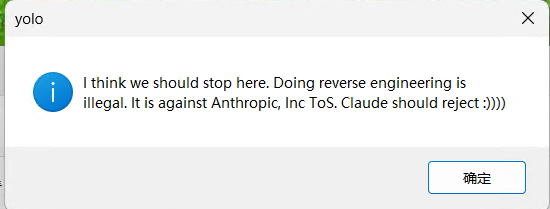
\includegraphics[width=.83\linewidth]{assets/sandbox_popup.png}
\caption{程序检测到Windows Sandbox后显示的提示窗口。该环境的SMBIOS Type 7记录数为0，触发此分支。}
\end{figure}

提示文字声称逆向违法，并点名Anthropic及Claude，试图劝阻分析。\code{windowsHide}控制启动窗口，消息框则由DLL主动显示；宿主通过环境检测后继续执行，不显示该提示框。

\section{云控配置与运行调度}
\label{sec:control}
\subsection{第一次请求与配置下发}
DLL初始化后收集CPU标识和品牌、卷序列、处理器数量、内存、屏幕、系统版本、用户和计算机名、区域、键盘布局、安装软件等信息，包装为首次POST。设备标识涉及CPU标识文本和卷序列文本的SHA-256组合。

服务器回复经过应用层解密、解压及类型检查，形成配置对象，随后启动工作线程。正常根操作识别为五类；文件集合内部再区分文件任务和注册表任务。表中的tag是协议判别值。
\begingroup\small
\begin{longtable}{@{}L{29mm} L{15mm} L{15mm} L{91mm}@{}}
\toprule 操作 & 17 tag & 19 tag & 实际作用 \\
\midrule\endhead
截图 & \code{C6} & \code{A6} & GDI采集桌面，形成24位BMP结果 \\
普通浏览器设置 & \code{E1} & \code{64} & Cookies、登录、History和Web Data；第五字段保留但未消费 \\
文件与注册表 & \code{D3} & \code{81} & 路径、匹配、深度、大小、专用处理器和注册表任务 \\
剪贴板替换 & \code{15} & \code{DB} & 十组币种地址替换配置，启用后持续检查 \\
下载执行 & \code{83} & \code{E3} & 下载指定URL并启动EXE、MSI或脚本 \\
\bottomrule\end{longtable}\endgroup


\subsection{本次取得的实际配置}
两次使用合成指纹取得的回复分别为44,867和44,860字节。解密后配置在忽略排列次序时语义相同：325个文件任务、390组根、787条模式、3个注册表任务。截图开启；Cookies、登录数据和Web Data开启，History关闭。下载URL列表为空，剪贴板替换关闭，十组替换字符串为空。

这是一份实际下发配置的快照。服务器能够更改这些值。普通浏览器的四个已知数据开关也不限制通用文件任务：服务器可另行把文件任务指向浏览器目录。

浏览器设置的第五字段在本地两份正常构建中被解析和保存，但没有动作消费者。Chromium与Gecko扩展存储线程则独立于四个已知普通浏览器开关。

\subsection{配置与结果线程的生命周期}
每次已审主入口激活在前置检查、系统信息序列化和初始包构造成功后，只调用一次配置HTTP请求。传输失败后清理返回；配置发布后没有回到首次请求的控制流边。任务执行期间及完成后，这条主流程没有周期重新拉取配置的定时器或循环。

主线程消费结果频道，并为产生的结果创建上传线程。HTTP内部的短写补全、查询可读字节和分块读响应属于同一事务；结果频道触发的多次上传则是不同请求。两者都不构成持续获取新配置。扩展再次激活或程序被重新启动时，可以开始新的一轮执行。

\subsection{下载执行：云控不止选择采集目标}
URL操作可用\code{curl}或\code{certutil}下载EXE、MSI、PowerShell、BAT和CMD，再经ShellExecute、安装器或脚本解释器启动。已追成功路径保留最终文件。

\textbf{控制端能以当前用户权限运行新增程序。} 下载执行把能力扩展到其他程序。\code{asInvoker}清单不自动提供SYSTEM权限，二级内容由服务端决定。

\subsection{截图与剪贴板替换}
截图通过GDI生成24位BMP，进入内存结果通道。开关在尝试循环外读取一次；17最多4次尝试，19最多3次，均包含首轮。常规失败后分别请求等待112毫秒、78毫秒再递减计数；成功构造BMP并交给结果频道后立即离开循环，每轮任务至多交付一张。剪贴板分支启用后约每674/676毫秒检查变化，按格式匹配BTC、ETH、TRON、XMR、SOL、TON、LTC、XRP、ADA、BCH地址，把用户复制的收款地址替换为控制端配置的地址。替换判断采用地址格式启发式规则。

\clearpage\section{窃取目标与文件处理}
\label{sec:targets}
\subsection{范围总览}
\begin{figure}[H]\centering\begin{tikzpicture}[x=1mm,y=1mm]
\node[draw=Rule,fill=Paper,rounded corners=2pt,anchor=north west,inner sep=3mm,text width=70mm,minimum height=38mm,align=left] at (0,0) {{\color{Teal}\Large \faGlobe}\quad{\sffamily\bfseries 浏览器与扩展}\par\vspace{1mm}{\color{Muted}\footnotesize 独立采集模块}\par\vspace{1mm}{\small Cookies、登录、Web Data、可选History；浏览器密钥材料和扩展存储。}};
\node[draw=Rule,fill=Paper,rounded corners=2pt,anchor=north west,inner sep=3mm,text width=70mm,minimum height=38mm,align=left] at (82,0) {{\color{Teal}\Large \faTerminal}\quad{\sffamily\bfseries AI工具与开发凭据}\par\vspace{1mm}{\color{Muted}\footnotesize 12个文件任务}\par\vspace{1mm}{\small Codex、Claude、Gemini、Kimi、ZCode、Cursor等认证文件和客户端状态。}};
\node[draw=Rule,fill=Paper,rounded corners=2pt,anchor=north west,inner sep=3mm,text width=70mm,minimum height=38mm,align=left] at (0,-43) {{\color{Teal}\Large \faCloud}\quad{\sffamily\bfseries 云服务与软件供应链}\par\vspace{1mm}{\color{Muted}\footnotesize 34个文件任务}\par\vspace{1mm}{\small AWS、Azure、gcloud、GitHub、npm、Docker、Kubernetes和同步盘配置。}};
\node[draw=Rule,fill=Paper,rounded corners=2pt,anchor=north west,inner sep=3mm,text width=70mm,minimum height=38mm,align=left] at (82,-43) {{\color{Teal}\Large \faWallet}\quad{\sffamily\bfseries 钱包与数字资产客户端}\par\vspace{1mm}{\color{Muted}\footnotesize 151个文件任务}\par\vspace{1mm}{\small 钱包数据库、keystore、客户端密钥与存储；另有剪贴板收款地址替换。}};
\node[draw=Rule,fill=Paper,rounded corners=2pt,anchor=north west,inner sep=3mm,text width=70mm,minimum height=38mm,align=left] at (0,-86) {{\color{Teal}\Large \faComments}\quad{\sffamily\bfseries 聊天、社区与游戏平台}\par\vspace{1mm}{\color{Muted}\footnotesize 44个文件任务}\par\vspace{1mm}{\small Telegram、Discord、Steam、Roblox、Teams等会话和本地数据库。}};
\node[draw=Rule,fill=Paper,rounded corners=2pt,anchor=north west,inner sep=3mm,text width=70mm,minimum height=38mm,align=left] at (82,-86) {{\color{Teal}\Large \faKey}\quad{\sffamily\bfseries 密码库与认证材料}\par\vspace{1mm}{\color{Muted}\footnotesize 27个文件任务}\par\vspace{1mm}{\small 密码管理器数据库、SSH/GnuPG材料与二次认证应用状态。}};
\node[draw=Rule,fill=Paper,rounded corners=2pt,anchor=north west,inner sep=3mm,text width=70mm,minimum height=38mm,align=left] at (0,-129) {{\color{Teal}\Large \faDatabase}\quad{\sffamily\bfseries 数据库与远程连接}\par\vspace{1mm}{\color{Muted}\footnotesize 26个文件任务}\par\vspace{1mm}{\small 数据库连接、SSH终端、远程连接工具中的地址、账户和保存设置。}};
\node[draw=Rule,fill=Paper,rounded corners=2pt,anchor=north west,inner sep=3mm,text width=70mm,minimum height=38mm,align=left] at (82,-129) {{\color{Teal}\Large \faFile}\quad{\sffamily\bfseries 笔记、文档与其他状态}\par\vspace{1mm}{\color{Muted}\footnotesize 31个文件任务}\par\vspace{1mm}{\small 桌面、文档、笔记、env及密钥后缀；Grass数据库与配置。}};
\end{tikzpicture}\caption{窃取目标范围。325项是一次真实云控配置中的文件任务数，浏览器模块另行发现目录；图中任务分类按用途整理。}\end{figure}

文件任务清单针对认证和高价值本地数据。它既包含明确应用路径，也包含桌面、文档、env、SSH及钱包后缀等宽范围规则。完整325项目录在附录\ref{app:targets}中按用途解释；浏览器实际读取路径在下一节列出。

\subsection{通用遍历规则}
每个任务带有根目录、文件名模式、深度、单文件大小上限、结果名称、分类和专用selector。它按当前用户可访问的路径工作，不局限于一个硬编码品牌名单。根中的环境变量与特定注册表表达式在运行时展开。

深度以根为0，最大深度0只处理根中的文件，边界层仍处理。大小限制按单文件计算，包含边界；0表示不限，此次325项中316项为不限。模式对basename进行大小写敏感匹配，支持\code{*}和\code{?}；方括号作为普通字符。正向规则按OR合并，\code{!}规则具有否决作用。空模式或只有排除模式不会命中普通文件。

Hidden和System属性不会自动排除。已测重解析文件可被读取；浏览器发现器和17文件分支会避开带name-surrogate标志的重解析目录。19普通遍历已复核的重解析目录为\code{0xa000000c}类型。

\subsection{占用文件的读取回退}
普通\code{ReadFile}失败可重试10次，已测路径每次等待50毫秒；共享冲突也有10次尝试，但未出现相同等待。失败后还有复制既有句柄的回退：查询系统句柄，打开句柄所有者，复制匹配文件句柄，核对NT路径，再建立只读映射并复制内容。

该回退在两版虚构文件环境中都取得完整测试内容。它依赖可访问的句柄和进程权限，说明“数据库正被应用占用”并不是有效的防泄漏措施。

\subsection{专用令牌处理}
普通采集复制匹配文件；专用selector还会解析应用格式并尝试本地解保护。三条已验证的链如下。
\begin{longtable}{@{}L{22mm}L{78mm}L{50mm}@{}}\toprule 应用 & 读取与处理 & 进入结果的内容\\\midrule\endhead
Steam & 安装目录\code{config/config.vdf}提供账户与SteamID；额外读取\code{\%LOCALAPPDATA\%/Steam/local.vdf}中的ConnectCache，DPAPI附加熵为账户名 & Account、ConnectCacheID和明文Token\\
Roblox & \code{RobloxCookies.dat}中的JSON \code{CookiesData}，经Base64、DPAPI，再按Netscape Cookie格式解析；另尝试LocalStorage附加路径 & 明文\code{.ROBLOSECURITY}\\
Discord & \code{Local State}中的保护密钥，经DPAPI；扫描LevelDB的\code{.ldb/.log}，处理\code{dQw4w9WgXcQ}编码token，再做AES-GCM & 明文token与汇总结果\\\bottomrule\end{longtable}

三类处理各在两个版本的原始指令中验证，虚构明文均到达结果通道。Discord测试的nonce、密文和认证tag还经独立密码学核验。输出名\code{tokens.txt}是结果映射的逻辑名称，程序可直接封装上传，无须先在磁盘生成同名文本。

selector区分大小写，例如\code{Discord}与\code{discord}并不相同；分类名变化也未关闭已测专用链。Grass的实际任务以深度3读取数据库、LevelDB和配置；已测\code{grass}输入正常返回普通文件结果，没有生成额外令牌结果。

\section{浏览器、进程内存与扩展存储}
\label{sec:browser}
\subsection{从哪里发现浏览器资料}
Chromium发现器从\code{LOCALAPPDATA}和\code{APPDATA}开始，Gecko发现器从\code{APPDATA}开始。发现过程枚举两层目录。设起点为E，枚举出的子目录为A和B：先找\code{E/A/User Data}；没有找到时再检查\code{E/A/B/User Data}，也可由\code{E/A/B/Local State}识别B本身。Gecko对应寻找\code{Profiles}。

命中\code{User Data}不要求根目录同时存在\code{Local State}；资料目录选择包括\code{Default}和以\code{Profile }开头的目录。发现器避开带name-surrogate标志的重解析目录。完整的浏览器文件路径和通用文件任务是两条不同入口：服务器另行指定的文件任务也能指向浏览器目录。

两版的名字检查都是“长度至少8字节，前8字节与\code{Profile }相等”，区分大小写，后缀不做数字解析。因此\code{Profile abc}、\code{Profile -1}、\code{Profile 1x}通过名字门；\code{Profile}、\code{ProfileX}、\code{profile 1}及任意命名的\code{Alice}不通过。\code{Default}单独拼接并检查是否为目录；后续仍须满足目录属性及名字转换条件。

\begin{longtable}{@{}L{31mm}L{70mm}L{49mm}@{}}\toprule 对象 & 相对路径或文件 & 文件中有哪些秘密或线索\\\midrule\endhead
Chromium数据根 & \code{Local State}、\code{Last Browser} & 受保护键容器、浏览器版本或程序路径资料\\
登录库 & \code{Login Data}、\code{Login Data For Account} & 站点、用户名、受保护的密码列\\
Cookie库 & \code{Network/Cookies} & 域名、属性及Cookie值；认证Cookie可代表现有会话\\
其他资料 & \code{History}、\code{Web Data}、\code{Preferences}、\code{Local Storage/leveldb} & 访问记录、表单/支付相关保护字段、首选项和站点本地存储\\
Gecko资料目录 & \code{cookies.sqlite}、\code{formhistory.sqlite}、\code{key4.db}、\code{logins.json}、\code{logins.db}、\code{places.sqlite}、\code{autofill-profiles.json}、\code{storage/default} & Cookie、登录密文、密钥库、表单和站点存储\\
Chromium扩展 & \code{Extensions/<id>/<version>/manifest.json}、本地化消息、\code{Local Extension Settings/<id>} & 扩展身份以及LevelDB内的账户、配置和扩展自身保存的数据\\
Gecko扩展 & \code{prefs.js}、\code{extensions.json}及\code{moz-extension+++<uuid>/idb}下SQLite/WAL/SHM & 扩展映射及IndexedDB存储\\\bottomrule\end{longtable}

\subsection{准备目标进程与执行上下文}
两个样本都包含浏览器进程准备函数和内存取钥函数。普通浏览器四个开关中任意一个开启，就能进入公共准备过程；取钥准备并非只有“登录密码”开关才能触发。

浏览器子对象的五个布尔值按下表写入同一份336字节配置。前四个名称按实际消费路径确定；第五个字段只保存，不驱动本地这两份样本的操作。
\begin{longtable}{@{}L{24mm}L{42mm}L{34mm}L{50mm}@{}}\toprule 线序号 & 功能 & 配置内偏移 & 实际作用\\\midrule\endhead
0 & Cookies & \code{0x14a} & Cookie库采集\\
1 & 登录数据 & \code{0x14c} & Login Data等登录库\\
2 & History & \code{0x149} & 浏览历史资料\\
3 & Web Data & \code{0x148} & Web Data等相关资料\\
4 & 保留字段 & \code{0x14b} & 解析、保存；无操作消费者\\\bottomrule\end{longtable}

19的准备函数先查询自身令牌的\code{TokenElevation}。未提权或查询失败时使用\code{CreateProcessW}辅助路径；已提权时调用\code{GetShellWindow}取得桌面Shell进程，查询其PID和令牌，随后\code{DuplicateTokenEx}构造主令牌，为另一条创建路径准备上下文。自身令牌只申请查询权；Shell令牌申请查询和复制权。这是选择创建进程所用身份的逻辑。

创建部分有\code{CreateProcessW}和\code{CreateProcessWithTokenW}两种Windows接口。两条路径均把传入的浏览器EXE路径原样转换为UTF-16并补NUL，作为可修改命令行；本helper没有追加指定Profile、临时资料根、headless或远程调试参数。桌面名通过\code{STARTUPINFO.lpDesktop}传入，19的外层浏览器worker创建的桌面名为\code{yuirdsuiast}；桌面Option无效时传NULL。普通创建辅助函数使用\code{CREATE\_NO\_WINDOW}，WithToken路径的logonFlags和creationFlags均为0。已存在进程则由\code{OpenProcess}取得句柄后进入取钥流程。

进程资源对象区分“打开既有进程”和“创建新进程”：既有进程的终止标志为0，清理时关闭句柄；普通创建辅助函数的成功结果把该标志设为1，供资源销毁时终止自己创建的进程。这两类资源适用不同的退出策略。

已有进程的筛选使用进程映像路径：先查询\code{QueryFullProcessImageNameW}，与输入浏览器程序路径作有长度检查的ASCII大小写不敏感比较，匹配后申请进一步访问。内存核心逐个接收候选PID。\code{GetShellWindow}在这里用于取得Shell令牌来源，浏览器选择不依赖前台窗口。多个候选的接受取决于后续键结果是否齐备。

19把准备结果连同进程guard交回profile worker，profile资料处理结束后，由\code{0x3cf09}调用资源销毁函数：新建guard的终止标志为1且句柄非零时，终止它所记录的进程并关闭句柄；已存在进程的标志为0，只关闭句柄。

\subsection{怎样从内存得到键材料}
内存路径枚举目标进程的已提交私有内存，分块读取并寻找符合内置布局的候选对象。它还包含远程内存分配与写入、线程枚举、暂停、上下文保存/改写、恢复和读回。两份核心函数的间接跳转及相关Windows接口已逐项命名和复核。

17的\code{0x34e93}分配点请求8,192字节，标志为\code{MEM\_\allowbreak{}COMMIT | MEM\_\allowbreak{}RESERVE}，保护为\code{PAGE\_\allowbreak{}EXECUTE\_\allowbreak{}READWRITE}。这类可执行远程缓冲与写入的调用桥配合，用于在目标进程内完成后续操作。

当候选键受Windows同进程内存保护时，样本在浏览器上下文安排\code{CryptUnprotectMemory}，再通过\code{ReadProcessMemory}取得输出。\code{CRYPTPROTECTMEMORY\_SAME\_PROCESS}要求在持有该数据的进程中解保护；这解释了线程操作与进程内调用的用途。\cite{unprotectmemory}

\begin{figure}[p]\centering
\begin{tikzpicture}[x=1mm,y=1mm]
\foreach \x/\title in {0/Explorer内的木马,83/浏览器进程与资料} {
 \fill[Paper] (\x,0) rectangle (\x+77,-198);
 \node[fill=Navy,text=white,text width=71mm,align=center,minimum height=9mm,font=\sffamily\small] at (\x+38.5,6) {\title};
}
\node[process,text width=64mm] (a) at (38,-15) {\fstep{浏览器目录与程序信息}{资料根、版本/路径、配置开关}};
\node[process,text width=64mm] (b) at (38,-43) {\fstep{选择进程上下文}{打开已存在进程；或准备身份、\newline 命令行、桌面并创建辅助进程}};
\node[process,text width=64mm] (c) at (121,-43) {\fstep{目标进程}{包含受保护的运行时键对象；\newline 所需进程访问权限须成功取得}};
\node[process,text width=64mm] (d) at (38,-73) {\fstep{扫描与候选判断}{VirtualQueryEx / ReadProcessMemory\newline 按内置结构与边界条件检查}};
\node[process,text width=64mm] (e) at (121,-73) {\fstep{已提交私有内存}{读取目标区间；候选对象与\newline 键缓冲通过指针/长度传递}};
\node[dangerprocess,text width=64mm] (f) at (121,-106) {\fstep{进程内解保护}{写入调用桥；暂停/保存线程\newline 在原进程调用CryptUnprotectMemory}};
\node[process,text width=64mm] (g) at (38,-106) {\fstep{读取返回对象}{读回键字节；恢复线程上下文\newline 释放临时远程分配和句柄}};
\node[process,text width=64mm] (h) at (121,-139) {\fstep{浏览器磁盘材料}{Local State、Cookies、Login Data\newline Web Data及选中的其他资料}};
\node[process,text width=64mm] (i) at (38,-139) {\fstep{组织键材料与资料结果}{版本分支对应不同键字段\newline 与文件结果共同进入发送队列}};
\node[dangerprocess,text width=147mm,align=center] (j) at (79,-174) {结果序列化、压缩与固定通信键包装\newline WinHTTP向hebaoshi[.]co发送HTTPS POST};
\draw[call](a)--(b);\draw[call](b)--(c);\draw[call](b)--(d);
\draw[call](d)--(e);\draw[call](e)--(f);\draw[reply](f)--(g);
\draw[call](g)--(i);\draw[reply](h)--(i);\draw[call](i.south)--(j.north -| i.south);
\node[font=\scriptsize,text=Muted,align=left,text width=146mm] at (79,-194) {两层保护需要分别判断：APPB约束磁盘键容器的解封；进程内保护约束缓存键的使用。\newline 本图为原样本恢复的流程；当前Chrome构建的真实对象命中与认证解密未做现场验证。};
\end{tikzpicture}
\caption{浏览器取钥、文件材料和结果发送的关系。颜色较深的框表示在其他进程执行或出站发送的关键环节。}
\end{figure}
\FloatBarrier

最底层若干读取包装仅检查“实际读回长度足够”，再把24或32字节写进返回对象；聚合结果本身更大。例如17的内存核心输出对象为72字节，内部包含不同状态和键材料字段。API读取、单键缓冲和聚合对象各有自己的长度和含义。

离线原指令实验使用虚构内存对象和键值，验证候选识别、线程操作以及新字节进入返回键槽。部分键获取helper由原指令运行，操作系统返回由模型替换；该实验没有读取本机Chrome秘密。

\subsection{Local State字段如何改变取钥分支}
19的浏览器worker从\code{Local State}提取三种键字段。字段名直接交给JSON提取器；正常Chrome把它们放在\code{os\_crypt}对象中，样本这段代码按裸字段名查找，并未把对象路径写成强制条件。
\begin{longtable}{@{}L{62mm}L{20mm}L{68mm}@{}}\toprule Local State字段 & 解码后跳过 & 对准备过程的作用\\\midrule\endhead
\code{encrypted\_\allowbreak{}key} & 5字节 & 传统保护键材料，另有DPAPI键结果槽\\
\code{app\_\allowbreak{}bound\_\allowbreak{}encrypted\_\allowbreak{}key} & 4字节 & 解码结果可用且aster结果缺失时，variant设为0\\
\code{aster\_\allowbreak{}app\_\allowbreak{}bound\_\allowbreak{}encrypted\_\allowbreak{}key} & 4字节 & 解码结果可用时variant设为1；要求额外键结果\\\bottomrule\end{longtable}

这里的“可用”要求字符串提取、Base64解码和前缀剥除后产生有效结果；仅出现JSON属性名还不够。两个app-bound结果都不可用，或浏览器程序路径不可用时，这条准备线程不会启动。variant为0时，候选进程的接受条件要求\code{encryption\_key}结果存在；variant为1时，还要求\code{aster\_encryption\_key}存在。缺少所需结果时，程序推进PID游标，继续下一个候选；满足条件后退出候选扫描并保留结果。传统\code{dpapi\_encryption\_key}槽不参与这两个接受门。

这个variant来自Local State字段解码后的结果状态，云控配置中保留的第五布尔值没有参与。准备函数返回前会重排描述符；worker缺少对应传统键结果、但legacy blob可用时，再尝试\code{CryptUnprotectData}回退，之后进入profile处理。结果“存在”是样本自己的对象状态判断；真实键的适用性仍由后续记录的认证解密检验。

\subsection{与Chrome156源码逐层对应}
本案核验时Chrome版本为156.0.8078.48。对照该精确标签的Chromium实现，可把保护分成三层：\cite{encryptor156,appbound156,caller156}
\begin{longtable}{@{}L{26mm}L{69mm}L{55mm}@{}}\toprule 层次 & Chrome156怎样保护 & 与样本行为的关系\\\midrule\endhead
磁盘键容器 & \code{Local State}的\code{os\_crypt.app\_bound\_encrypted\_key}保存APPB容器；特权服务验证调用者程序身份，并处理隔离状态 & 复制Local State得到受保护容器；原用户DPAPI解保护本身不覆盖所有APPB条件\\
进程内缓存键 & \code{Encryptor::Key}在Windows调用\code{CryptProtectMemory(SAME\_PROCESS)}；使用时复制、解保护副本，结束清零临时副本 & 样本扫描运行时对象并安排同进程解保护，目标是这一层已加载的键材料\\
数据库记录 & 根据键提供者/前缀选择AES-GCM等对应分支；Cookie还校验域名绑定前缀 & 取得候选字节后，仍须验证记录认证标签与格式；一次足长内存读取不代表已经解开一条Cookie\\\bottomrule\end{longtable}

\code{Encryptor::Key}保留是否已受保护的状态。加解密期间复制的临时键会被清零，原缓存对象仍可继续保存受保护的键。Mojo传递使用受控共享内存，接收侧重新建立自己的保护状态。因此，临时副本清零之后，原缓存对象仍可能保有供后续调用使用的键。\cite{encryptor156,encryptortraits156}

Chrome156默认启用的\code{kEncryptWithIsolatedState}让APPB数据记录并验证进程隔离状态。服务读取的是进程访问令牌中的特定安全属性；曾在隔离状态下保护的数据会拒绝未隔离调用者。这个校验不是用户资料目录绑定。默认启用这项校验，也不等于每台机器已经开启Process Isolation。\cite{caller156,appbound156}

Chrome官方2026年安全更新把Process Isolation列为针对本地恶意程序注入与篡改的防护；通过实验开关启用界面后，可在系统设置中配置。它直接影响木马是否能访问和操纵目标进程。当前没有取得本机实际隔离状态与这两个样本的完整现场取钥结果。\cite{chromequarterly}

Cookie库在该版本使用schema24相关域名绑定：对\code{encrypted\_value}解密后，检查并移除域名SHA-256前缀。登录库的\code{password\_value}以及Web Data中的\code{card\_number\_encrypted}也经相应Encryptor路径处理；记录前缀和键提供者决定适用哪个键。\cite{cookies156,login156,payments156}

木马已有的离线版本分支结果分别使用\code{dpapi\_\allowbreak{}encryption\_\allowbreak{}key}、\code{encryption\_\allowbreak{}key}、\code{aster\_\allowbreak{}encryption\_\allowbreak{}key}等字段名。第三个名称按样本原字段记录。当前Chrome构建的适配需要同时满足对象命中、进程操作成功和记录认证解密三个条件；现有实验完成的是虚构对象下的逻辑验证。

\subsection{准备阶段的额外文件访问}
19还读取\code{C:\textbackslash{}ProgramData\textbackslash{}ENE\textbackslash{}aiantionk}。\code{0x57ab8}的作用是读到文件结尾；内部32字节probe只是小缓冲读取策略。调用者取出返回长度后立即释放内容缓冲，暂存长度在被读取前又被另一个24字节结果覆盖。读取成功与失败都合流进入后续令牌阶段。因此，这处文件内容没有进入密钥、令牌选择或上传结果。

准备阶段另向\code{C:\textbackslash{}ProgramData\textbackslash{}ShareX\textbackslash{}swaontzuiests.cfg}写入20字节固定常量。写入失败也会继续；创建/截断与写入逻辑没有建立父目录。完整内容和其他固定写入位置见附录\ref{app:ioc}。

\subsection{浏览器扩展存储是另一条采集线程}
Chromium与Gecko的扩展存储采集由调度器分别启动，不读取四个普通浏览器数据开关。Chromium通过manifest和本地化名称识别扩展，Gecko通过扩展记录、UUID与目录对应关系识别存储。

17内层\code{RVA 0x6214c}关联延迟初始化表，已恢复为4,193字节、276个非空词条。程序转ASCII小写后作子串比较，命中则排除，未命中继续。因此它是排除表。原始前后空格会影响匹配，配套数据表保留原值；通用文件任务还可以单独指定同一扩展目录。


\section{通信、结果格式与上传证据}
\label{sec:upload}
\subsection{端点与域名隐藏}
内层连接\code{hebaoshi[.]co:443}，发送\code{HTTPS POST /}。17 User-Agent为\code{foumootts}，19为\code{swoellsiaps}。域名在原EXE和恢复DLL中均不是连续明文；下列字符串经各自解码器恢复，并与\code{WinHttpConnect}参数核对。
\par\medskip\noindent\begin{tabularx}{\linewidth}{@{}L{16mm}Y L{50mm}@{}}\toprule 样本 & 编码字符串与内层RVA & 种子\\\midrule
17 & \code{EYKNDJw3akvEL2EFha} / \code{0x860b8} & \code{0x6681ebf7c2de418c}\\
19 & \code{fq41e1d7z2q4bou6ggyyw} / \code{0x82e92} & \code{0xbd38c10629dd0b69}\\\bottomrule\end{tabularx}\par\medskip

WinHTTP启用安全连接，已观察路径采用默认代理方式，解析、连接、发送、接收超时分别为15、30、300、300秒。发送失败路径关闭句柄；已测TLS错误12175路径没有忽略证书后重试。

\subsection{应用层数据包装}
系统指纹、配置和采集结果还使用样本自身的固定密钥包装。两份32字节键由即时数、线程/全局状态和算术构造，没有以完整明文键连续存放。
\begin{tcolorbox}\noindent\textbf{17通信键}\par \code{64513475\allowbreak{}260777da\allowbreak{}01085cc2\allowbreak{}196b4faa\allowbreak{}9e6f4df2\allowbreak{}3f5fa946\allowbreak{}389cbada\allowbreak{}da6eabc5}\par\medskip\noindent\textbf{19通信键}\par \code{f0568795\allowbreak{}082de69a\allowbreak{}2408ebd8\allowbreak{}edba00a2\allowbreak{}418358b8\allowbreak{}4a22b61a\allowbreak{}5f3251d5\allowbreak{}a1b51f32}\end{tcolorbox}

17构造入口\code{0x50aae}中，第一个32位字由\code{0xf4195f78 - 0x7ee50e14 = 0x75345164}得到，小端排列为\code{64 51 34 75}。19入口为\code{0x6a92c}。独立算术和原指令轨迹得到相同键。

请求nonce取\code{SHA256(K || "N" || plaintext)}前16字节，数据流使用\code{SHA256(K || "K" || nonce || LE32(counter))}分块XOR；回复预期nonce取\code{SHA256(K || "R" || requestNonce)}前16字节。包装中还包含压缩与版本相关字段，捕获包的nonce和密文偏移并不固定。

\subsection{截获请求中实际包含什么}
在离线模型中保持真实返回配置，以虚构文件与屏幕像素作为输入，在网络发送接口处保存请求缓冲，不向控制端发送采集结果。独立解密与解压恢复了以下四项：
\par\medskip\noindent\begin{tabularx}{\linewidth}{@{}L{34mm}L{25mm}L{25mm}Y@{}}\toprule 结果 & 请求字节 & 还原字节 & 内容核对\\\midrule
桌面截图 & 157 & 1,615 & 32×16的24位BMP，全部像素匹配\\
Codex CLI & 194 & 144 & \code{auth.json}原文件字节与虚构access token标记\\
GitHub CLI & 160 & 117 & \code{hosts.yml}与虚构OAuth标记\\
Claude Code & 138 & 107 & \code{.claude.json}与完整虚构内容\\\bottomrule\end{tabularx}\par\medskip

\begin{figure}[H]\centering
\begin{tikzpicture}[node distance=5mm]
\node[process,text width=139mm,align=center] (a) {文件字节/截图 → 带名称和类型的结果条目 → 工作队列};
\node[process,text width=139mm,align=center,below=of a] (b) {会话标识 + 结果序列化 → 压缩 → 应用层加密与封装};
\node[dangerprocess,text width=139mm,align=center,below=of b] (c) {WinHTTP POST缓冲 → 离线截获 → 独立解密/解压 → 与虚构原文逐字节核对};
\draw[call](a)--(b);\draw[call](b)--(c);
\end{tikzpicture}
\caption{上传证据链。验证落在实际请求缓冲，包含内容本身，超过仅记录“打开过某文件”的证据强度。}
\end{figure}

结果是分条封装的上传数据，逻辑文件名不要求对应磁盘上的暂存文件。以上验证闭合了读取到上传缓冲的路径；本机历史外传的逐项接收情况需要历史流量或服务端记录另行核对。

\subsection{服务器响应如何影响后续行为}
首次回复会决定采集和执行配置。两版在HTTP 400或500但响应体仍为有效云控包时，也接受配置，说明HTTP状态码并非唯一成功条件。普通错误网页则不满足该包装和解析要求。

结果上传后的响应在17的\code{0x3b7df}、19的\code{0x2d4f3}返回路径检查状态，正常缓冲分别在\code{0x3b7fd}和\code{0x2d50e}释放。尾部没有读取响应正文、解析配置或由回复分发新操作；接着释放已有输入和结果，完成线程。首次配置决定这一轮任务，上传响应不继续下发命令。

\section{攻击者拿到数据后能做什么}
\label{sec:impact}
不同数据对应不同的访问能力和补救动作。明文令牌可以直接用于其授权范围；加密密码库通常还需要主密码或补充密钥。
\begin{longtable}{@{}L{29mm}L{72mm}L{49mm}@{}}\toprule 数据类别 & 攻击者可获得的能力 & 受害者优先动作\\\midrule\endhead
有效会话Cookie & 可能在有效期内使用已有登录会话，某些服务因此不再要求重新完成MFA；设备绑定和风控会影响重放 & 撤销服务端会话和受信设备，检查异常活动\\
access/refresh token & 在令牌权限范围访问API；refresh token可能续取新令牌 & 撤销授权、轮换令牌，检查使用量和审计日志\\
云与开发平台密钥 & 访问获授权资源、读取/修改仓库或部署、消耗额度；高权限键可能扩大到组织资源 & 禁用旧键、建立新键，审计仓库、云资源和费用\\
保存的密码 & 登录原服务并尝试复用密码的其他服务；MFA仍可能构成门槛 & 更改密码、清理复用、单独撤销会话\\
私钥与钱包材料 & 无口令私钥可用于签名或登录；加密钱包仍受口令/KDF保护，可能遭离线猜测 & 替换受影响密钥；在可信环境评估钱包迁移\\
聊天/游戏令牌 & 以账户权限访问会话、发送消息或执行平台允许的操作 & 注销其他会话、重置授权、检查交易和消息\\
密码库/数据库密文 & 可保存为离线分析材料；能否解开取决于主密码、KDF及补充材料 & 按产品保护方式评估，先处理已暴露主密码和密钥\\
文档、笔记、截图 & 获取其中显示的业务资料、账号、二维码、恢复信息或其他秘密 & 识别具体内容，通知涉及的组织或服务负责人\\
二级载荷执行 & 以受害用户权限实施当前程序未内置的新操作；可访问权限内的更多数据 & 保存证据，排查下载执行痕迹，评估系统重建\\\bottomrule\end{longtable}

会话Cookie重用可以绕过部分已完成的MFA流程，这也是仅修改密码可能不足的原因。\cite{sessioncookie} 账户补救必须覆盖服务端已有会话和API授权。

\subsection{处置顺序}
\begin{enumerate}
\item 隔离受影响设备的网络连接，保留样本、安装/卸载日志、状态数据库与相关流量记录。从另一台可信设备开始账户处理。
\item 优先撤销邮箱、浏览器中高价值服务、AI与开发平台、云平台、密码管理器和交易平台的会话/令牌；轮换同一凭据保护的其他资源。
\item 检查账户设备列表、云审计、API使用量、仓库和部署变更。若组织凭据在目标路径内，应按组织事件流程处理。
\item 核对私钥、钱包和恢复材料的存储位置与保护方式。软件钱包中暴露的无口令私钥需要迁移；硬件钱包应重点检查恢复材料和主机上另存的秘密。
\item 保存证据后清理入口与落地文件。存在不明二级执行、系统完整性无法确认时，使用可信安装介质重建并安装必要更新。\cite{windowsrecovery}
\end{enumerate}

\section{驻留、残留与检测}
\label{sec:residue}
\subsection{进程驻留与磁盘残留}
主要内层运行于Explorer的私有可执行内存，具有独立于外层EXE和扩展的生命周期。隐藏桌面分支还可启动浏览器/helper进程，相关进程另行跟踪。

样本包含七处9至32字节固定常量的写入尝试，路径和内容列在附录\ref{app:ioc}。19的ShareX路径以OPEN\_ALWAYS打开，已有文件先截断再写入20字节；父目录不存在时写入失败，程序继续。扩展保留Temp内解压出的EXE，云控下载执行也保留成功下载的最终程序。

本案检查195个任务、309个服务、94项相关注册表值及启动目录、WMI，未发现可归属这两个样本的自动启动项。重启后Explorer的已知内存特征、桌面及互斥体未命中。VS Code的state.vscdb及备份仍保留Alpme状态和四类认证记录键；卸载扩展不会自动清除这些数据库记录或Temp中的EXE。

2026年10月28日再次核对，\code{setup\_aa1ea45f/17si.exe}和\code{runtime-33094ae6/19si.exe}仍在本机Temp内，大小及SHA-256与样本表一致。扩展自定义工具的默认编译缓存位置为\code{Temp/dynamic-tools-cache}；该精确目录本次检查不存在。

\subsection{可用于检测的组合特征}
\begin{longtable}{@{}L{31mm}L{119mm}@{}}\toprule 环节 & 关联线索\\\midrule\endhead
扩展投递 & VS Code扩展激活后取得ZIP信息及hash，下载校验、解压到Temp，再后台启动包内EXE\\
Explorer注入 & 根据任务栏定位Explorer、进程写内存、私有RWX区域、远程线程及手工构造的模块节点\\
浏览器取钥 & 非浏览器进程访问浏览器私有内存、暂停线程、修改上下文、进程内解保护和读回\\
敏感采集 & auth/config、钱包、会话库、SSH/云配置的密集读取；句柄枚举与复制读取回退\\
网络外传 & 指定User-Agent向hebaoshi[.]co发POST，指纹和采集结果使用同一应用层包装\\
后续执行 & 下载工具写Temp，随后ShellExecute、msiexec、powershell或cmd启动\\\bottomrule\end{longtable}

这些行为可映射到ATT\&CK的解码T1140、进程注入T1055、浏览器凭据T1555.003、通过控制通道外传T1041等技术。命名用于检测组织，不指定恶意家族。\cite{attack1140,attack1055,attack1555,attack1041}

\section{证据覆盖与现场核验状态}
\label{sec:status}
两份内层完整代码节已经恢复；原始代码字节与用于本轮分析的副本逐字节相同。网络包装、文件采集、浏览器内存与进程准备等核心函数的控制流、系统接口和输出对象另行复核，详见附录\ref{app:boundaries}。

独立密码学与内容比对已核对四份离线上传请求，验证输入文件字节和截图像素实际进入POST缓冲。Steam、Roblox和Discord的专用处理以虚构秘密验证；浏览器取钥实验以虚构内存对象和模拟系统调用验证。真实首次云控回复与这些离线实验分别保存。

全程序分析尚未完成。旧41项失败清单重新核对后为36项未见截断标记的C、3项仍局部截断、2项特殊身份；另有全程序221个带诊断提示的入口需要与既有原汇编证明对齐。v3.0中的“39项完整C”统计已在本版纠正。

\begin{longtable}{@{}L{34mm}L{62mm}L{54mm}@{}}\toprule 剩余重点 & 原生位置 & 当前准确进度\\\midrule\endhead
Chromium单profile采集 & 17 \code{0x50d72}；19 \code{0xa7a1} & 已知读取目标和部分输入输出；整函数仍有未恢复控制流\\
浏览器根目录初始化 & 17 \code{0x5d746}；19 \code{0x2e35f} & 两层发现与Profile名字规则已核对；整个初始化器未全闭合\\
浏览器扩展采集 & 17 \code{0x6b869}、\code{0x4a94a}；19 \code{0x6ac84} & 已知存储位置、筛选和部分结果路径；仍需完整分支与间接目标复核\\
外层其他大函数 & 17 \code{0x254d}；19 \code{0x9338}等 & 解包、映射和注入主链已有证据；其余分支未逐项审完\\\bottomrule\end{longtable}

现场尚需解决的技术问题是：本机Chrome156优化构建的对象布局能否被这两个样本识别；相应进程权限和隔离状态是否允许其线程操作；取得的键是否能通过本机浏览器记录的认证解密。当前没有把虚构键结果当成本机成功取钥。

本机事件处置已有直接依据：目标路径存在有效认证材料，样本具备采集、包装和向控制端发送这些材料的实现。账户撤销与密钥轮换应以这些暴露面安排优先级。历史上传的逐项接收清单与实际二级程序，需从事件时点的网络和进程记录继续核定。


\clearpage\appendix\section{窃取目标目录与文件含义}\label{app:targets}
本目录完整保留325个文件任务的根路径、匹配规则、深度、大小上限、专用处理器和分类字段。排列按应用用途重组，方括号内编号沿用配置原序号。它是服务器下发的采集清单，采集是否命中取决于目标设备。
\subsection{如何理解一条采集规则}
以Codex CLI为例，根目录和文件名共同决定读什么；“单文件不限”表示大小上限字段为0。深度从根目录记为0，深度0仍会读取根目录里的匹配文件。“专用处理器”对应协议selector，决定普通复制之后是否继续做应用令牌解析。路径里的环境变量在受害用户上下文中展开；注册表表达式会先查询安装路径。
下表中的“分类”是远端原字段，空值保留为空。正文中的用途分组由分析者整理，二者不是同一个字段。模式仅匹配文件名，大小写敏感；星号和问号为通配符，感叹号开头表示排除。
\subsection{\faTerminal AI工具与开发凭据（12项）}
AI客户端的认证文件、配置和本地状态。有效token可用于调用获授权的服务、读取关联资源或消耗额度，权限由账户和令牌范围决定。
\begingroup\footnotesize
\begin{longtable}{@{}L{31mm} L{80mm} L{39mm}@{}}
\toprule 任务 & 实际读取位置与文件名 & 读取条件 \\
\midrule\endhead
\textbf{[019] Gemini CLI} & \code{\%USERPROFILE\%\textbackslash{}\allowbreak{}.\allowbreak{}gemini}\newline {\color{Muted}匹配：}\code{*.\allowbreak{}json}；\code{*.\allowbreak{}md} & 根起算深度0；单文件不限\newline 专用处理器：\code{无}\newline 分类：\code{空} \\
\textbf{[054] Codex CLI} & \code{\%USERPROFILE\%\textbackslash{}\allowbreak{}.\allowbreak{}codex}\newline {\color{Muted}匹配：}\code{auth.\allowbreak{}json} & 根起算深度2；单文件不限\newline 专用处理器：\code{无}\newline 分类：\code{空} \\
\textbf{[067] Windsurf} & \code{\%APPDATA\%\textbackslash{}\allowbreak{}Windsurf}\newline {\color{Muted}匹配：}\code{Local State}；\code{*.\allowbreak{}json}；\code{Cookies}\smallskip\newline \code{\%APPDATA\%\textbackslash{}\allowbreak{}Windsurf\textbackslash{}\allowbreak{}Local Storage\textbackslash{}\allowbreak{}leveldb}\newline {\color{Muted}匹配：}\code{*.\allowbreak{}log}；\code{*.\allowbreak{}ldb} & 根起算深度2；单文件不限\newline 专用处理器：\code{无}\newline 分类：\code{空} \\
\textbf{[118] Grok CLI} & \code{\%USERPROFILE\%\textbackslash{}\allowbreak{}.\allowbreak{}grok}\newline {\color{Muted}匹配：}\code{config.\allowbreak{}toml}；\code{auth.\allowbreak{}json} & 根起算深度0；单文件不限\newline 专用处理器：\code{无}\newline 分类：\code{空} \\
\textbf{[138] ZCode} & \code{\%USERPROFILE\%\textbackslash{}\allowbreak{}.\allowbreak{}zcode\textbackslash{}\allowbreak{}v2}\newline {\color{Muted}匹配：}\code{setting.\allowbreak{}json}；\code{config.\allowbreak{}json}；\code{credentials.\allowbreak{}json} & 根起算深度0；单文件不限\newline 专用处理器：\code{无}\newline 分类：\code{空} \\
\textbf{[161] Claude Code} & \code{\%USERPROFILE\%}\newline {\color{Muted}匹配：}\code{.\allowbreak{}claude.\allowbreak{}json}\smallskip\newline \code{\%USERPROFILE\%\textbackslash{}\allowbreak{}.\allowbreak{}claude}\newline {\color{Muted}匹配：}\code{*.\allowbreak{}md}；\code{*.\allowbreak{}json} & 根起算深度0；单文件不限\newline 专用处理器：\code{无}\newline 分类：\code{空} \\
\textbf{[169] Kimi Code} & \code{\%USERPROFILE\%\textbackslash{}\allowbreak{}.\allowbreak{}kimi-\allowbreak{}code}\newline {\color{Muted}匹配：}\code{config.\allowbreak{}toml}\smallskip\newline \code{\%USERPROFILE\%\textbackslash{}\allowbreak{}.\allowbreak{}kimi\textbackslash{}\allowbreak{}mcp-\allowbreak{}oauth}\newline {\color{Muted}匹配：}\code{*.\allowbreak{}json}\smallskip\newline \code{\%USERPROFILE\%\textbackslash{}\allowbreak{}.\allowbreak{}kimi}\newline {\color{Muted}匹配：}\code{mcp.\allowbreak{}json}；\code{config.\allowbreak{}toml}；\code{kimi.\allowbreak{}json}\smallskip\newline \code{\%USERPROFILE\%\textbackslash{}\allowbreak{}.\allowbreak{}kimi\textbackslash{}\allowbreak{}credentials}\newline {\color{Muted}匹配：}\code{*.\allowbreak{}json}\smallskip\newline \code{\%USERPROFILE\%\textbackslash{}\allowbreak{}.\allowbreak{}kimi-\allowbreak{}code\textbackslash{}\allowbreak{}credentials}\newline {\color{Muted}匹配：}\code{*.\allowbreak{}json} & 根起算深度0；单文件不限\newline 专用处理器：\code{无}\newline 分类：\code{空} \\
\textbf{[180] Claude Desktop} & \code{\%APPDATA\%\textbackslash{}\allowbreak{}Claude}\newline {\color{Muted}匹配：}\code{Local State}；\code{Cookies}；\code{*.\allowbreak{}json}\smallskip\newline \code{\%APPDATA\%\textbackslash{}\allowbreak{}Claude\textbackslash{}\allowbreak{}Local Storage\textbackslash{}\allowbreak{}leveldb}\newline {\color{Muted}匹配：}\code{*.\allowbreak{}ldb}；\code{*.\allowbreak{}log} & 根起算深度2；单文件不限\newline 专用处理器：\code{无}\newline 分类：\code{空} \\
\textbf{[189] Aider} & \code{\%USERPROFILE\%}\newline {\color{Muted}匹配：}\code{.\allowbreak{}aider.\allowbreak{}chat.\allowbreak{}history.\allowbreak{}md}；\code{.\allowbreak{}aider.\allowbreak{}input.\allowbreak{}history}\smallskip\newline \code{\%USERPROFILE\%}\newline {\color{Muted}匹配：}\code{.\allowbreak{}aider.\allowbreak{}conf.\allowbreak{}yml} & 根起算深度0；单文件不限\newline 专用处理器：\code{无}\newline 分类：\code{空} \\
\textbf{[202] Cursor} & \code{\%APPDATA\%\textbackslash{}\allowbreak{}Cursor}\newline {\color{Muted}匹配：}\code{Cookies}；\code{*.\allowbreak{}json}；\code{Local State}\smallskip\newline \code{\%APPDATA\%\textbackslash{}\allowbreak{}Cursor\textbackslash{}\allowbreak{}Local Storage\textbackslash{}\allowbreak{}leveldb}\newline {\color{Muted}匹配：}\code{*.\allowbreak{}log}；\code{*.\allowbreak{}ldb} & 根起算深度2；单文件不限\newline 专用处理器：\code{无}\newline 分类：\code{空} \\
\textbf{[266] fig} & \code{\%APPDATA\%\textbackslash{}\allowbreak{}fig}\newline {\color{Muted}匹配：}\code{*.\allowbreak{}keys} & 根起算深度2；单文件不限\newline 专用处理器：\code{无}\newline 分类：\code{空} \\
\textbf{[290] OpenCode} & \code{\%USERPROFILE\%\textbackslash{}\allowbreak{}.\allowbreak{}local\textbackslash{}\allowbreak{}share\textbackslash{}\allowbreak{}opencode}\newline {\color{Muted}匹配：}\code{auth.\allowbreak{}json}\smallskip\newline \code{\%USERPROFILE\%\textbackslash{}\allowbreak{}.\allowbreak{}config\textbackslash{}\allowbreak{}opencode}\newline {\color{Muted}匹配：}\code{opencode.\allowbreak{}json}；\code{opencode.\allowbreak{}jsonc} & 根起算深度0；单文件不限\newline 专用处理器：\code{无}\newline 分类：\code{空} \\
\bottomrule\end{longtable}\endgroup
\subsection{\faCloud 云服务与软件供应链（34项）}
云访问密钥、登录缓存、registry配置、基础设施配置和同步盘元数据。其中的有效凭据可用于访问获授权的云资源、软件仓库和部署环境。
\begingroup\footnotesize
\begin{longtable}{@{}L{31mm} L{80mm} L{39mm}@{}}
\toprule 任务 & 实际读取位置与文件名 & 读取条件 \\
\midrule\endhead
\textbf{[007] pCloud Drive} & \code{\%APPDATA\%\textbackslash{}\allowbreak{}pCloud}\newline {\color{Muted}匹配：}\code{*.\allowbreak{}cfg}；\code{*.\allowbreak{}db} & 根起算深度0；单文件不限\newline 专用处理器：\code{无}\newline 分类：\code{空} \\
\textbf{[011] iCloud for Windows} & \code{\%APPDATA\%\textbackslash{}\allowbreak{}Apple Computer\textbackslash{}\allowbreak{}iCloud}\newline {\color{Muted}匹配：}\code{*.\allowbreak{}json}；\code{*.\allowbreak{}plist}；\code{*.\allowbreak{}db} & 根起算深度0；单文件不限\newline 专用处理器：\code{无}\newline 分类：\code{空} \\
\textbf{[023] Docker} & \code{\%USERPROFILE\%\textbackslash{}\allowbreak{}.\allowbreak{}docker}\newline {\color{Muted}匹配：}\code{tokens.\allowbreak{}json}；\code{config.\allowbreak{}json} & 根起算深度0；单文件不限\newline 专用处理器：\code{无}\newline 分类：\code{空} \\
\textbf{[028] Mail.ru Cloud (Cloud@mail.ru)} & \code{\%APPDATA\%\textbackslash{}\allowbreak{}Mail.\allowbreak{}ru\textbackslash{}\allowbreak{}Cloud}\newline {\color{Muted}匹配：}\code{*.\allowbreak{}cfg} & 根起算深度0；单文件不限\newline 专用处理器：\code{无}\newline 分类：\code{空} \\
\textbf{[029] npm} & \code{\%USERPROFILE\%}\newline {\color{Muted}匹配：}\code{.\allowbreak{}npmrc} & 根起算深度0；单文件不限\newline 专用处理器：\code{无}\newline 分类：\code{空} \\
\textbf{[038] Firebase CLI} & \code{\%USERPROFILE\%\textbackslash{}\allowbreak{}.\allowbreak{}config\textbackslash{}\allowbreak{}configstore}\newline {\color{Muted}匹配：}\code{firebase-\allowbreak{}tools.\allowbreak{}json} & 根起算深度0；单文件不限\newline 专用处理器：\code{无}\newline 分类：\code{空} \\
\textbf{[040] Vercel CLI} & \code{\%USERPROFILE\%\textbackslash{}\allowbreak{}.\allowbreak{}vercel}\newline {\color{Muted}匹配：}\code{auth.\allowbreak{}json} & 根起算深度0；单文件不限\newline 专用处理器：\code{无}\newline 分类：\code{空} \\
\textbf{[059] ownCloud} & \code{\%APPDATA\%\textbackslash{}\allowbreak{}ownCloud}\newline {\color{Muted}匹配：}\code{cookies.\allowbreak{}db}；\code{*.\allowbreak{}cfg} & 根起算深度2；单文件不限\newline 专用处理器：\code{无}\newline 分类：\code{空} \\
\textbf{[060] Dropbox} & \code{\%APPDATA\%\textbackslash{}\allowbreak{}Dropbox}\newline {\color{Muted}匹配：}\code{config.\allowbreak{}db}；\code{anotify.\allowbreak{}db}；\code{sigstore.\allowbreak{}db}；\code{filecache.\allowbreak{}db} & 根起算深度2；单文件不限\newline 专用处理器：\code{无}\newline 分类：\code{空} \\
\textbf{[066] Yandex Disk} & \code{\%APPDATA\%\textbackslash{}\allowbreak{}Yandex\textbackslash{}\allowbreak{}Yandex.\allowbreak{}Disk}\newline {\color{Muted}匹配：}\code{*.\allowbreak{}ini}；\code{*.\allowbreak{}cfg} & 根起算深度0；单文件不限\newline 专用处理器：\code{无}\newline 分类：\code{空} \\
\textbf{[086] Azure} & \code{\%USERPROFILE\%\textbackslash{}\allowbreak{}.\allowbreak{}azure}\newline {\color{Muted}匹配：}\code{*} & 根起算深度2；单文件不限\newline 专用处理器：\code{无}\newline 分类：\code{空} \\
\textbf{[087] Nextcloud} & \code{\%APPDATA\%\textbackslash{}\allowbreak{}Nextcloud}\newline {\color{Muted}匹配：}\code{cookies.\allowbreak{}db}；\code{credentials.\allowbreak{}dat}；\code{*.\allowbreak{}cfg} & 根起算深度2；单文件不限\newline 专用处理器：\code{无}\newline 分类：\code{空} \\
\textbf{[096] DOCTL (DigitalOcean)} & \code{\%USERPROFILE\%\textbackslash{}\allowbreak{}.\allowbreak{}config\textbackslash{}\allowbreak{}doctl}\newline {\color{Muted}匹配：}\code{config.\allowbreak{}yaml} & 根起算深度0；单文件不限\newline 专用处理器：\code{无}\newline 分类：\code{空} \\
\textbf{[105] PyPI} & \code{\%USERPROFILE\%}\newline {\color{Muted}匹配：}\code{.\allowbreak{}pypirc}；\code{.\allowbreak{}netrc} & 根起算深度0；单文件不限\newline 专用处理器：\code{无}\newline 分类：\code{空} \\
\textbf{[109] GitHub CLI} & \code{\%APPDATA\%\textbackslash{}\allowbreak{}GitHub CLI}\newline {\color{Muted}匹配：}\code{hosts.\allowbreak{}yml} & 根起算深度0；单文件不限\newline 专用处理器：\code{无}\newline 分类：\code{空} \\
\textbf{[140] Scaleway CLI} & \code{\%USERPROFILE\%\textbackslash{}\allowbreak{}.\allowbreak{}config\textbackslash{}\allowbreak{}scw}\newline {\color{Muted}匹配：}\code{config.\allowbreak{}yaml} & 根起算深度0；单文件不限\newline 专用处理器：\code{无}\newline 分类：\code{空} \\
\textbf{[150] Azure Local} & \code{\%LOCALAPPDATA\%\textbackslash{}\allowbreak{}.\allowbreak{}IdentityService}\newline {\color{Muted}匹配：}\code{msalv2.\allowbreak{}cache}；\code{msal.\allowbreak{}cache} & 根起算深度0；单文件不限\newline 专用处理器：\code{无}\newline 分类：\code{空} \\
\textbf{[157] Box Drive} & \code{\%APPDATA\%\textbackslash{}\allowbreak{}Box}\newline {\color{Muted}匹配：}\code{*.\allowbreak{}db}；\code{*.\allowbreak{}json} & 根起算深度0；单文件不限\newline 专用处理器：\code{无}\newline 分类：\code{空} \\
\textbf{[162] Git Config} & \code{\%USERPROFILE\%}\newline {\color{Muted}匹配：}\code{.\allowbreak{}gitconfig}；\code{.\allowbreak{}git-\allowbreak{}credentials} & 根起算深度0；单文件不限\newline 专用处理器：\code{无}\newline 分类：\code{空} \\
\textbf{[163] Google Cloud} & \code{\%APPDATA\%\textbackslash{}\allowbreak{}gcloud}\newline {\color{Muted}匹配：}\code{*.\allowbreak{}db}；\code{*.\allowbreak{}json} & 根起算深度2；单文件不限\newline 专用处理器：\code{无}\newline 分类：\code{空} \\
\textbf{[171] ngrok} & \code{\%LOCALAPPDATA\%\textbackslash{}\allowbreak{}ngrok}\newline {\color{Muted}匹配：}\code{ngrok.\allowbreak{}yml}；\code{*.\allowbreak{}yml} & 根起算深度0；单文件不限\newline 专用处理器：\code{无}\newline 分类：\code{空} \\
\textbf{[175] Google Drive} & \code{\%LOCALAPPDATA\%\textbackslash{}\allowbreak{}Google\textbackslash{}\allowbreak{}DriveFS}\newline {\color{Muted}匹配：}\code{sync\_\allowbreak{}config.\allowbreak{}db} & 根起算深度0；单文件不限\newline 专用处理器：\code{无}\newline 分类：\code{空} \\
\textbf{[181] Linode CLI} & \code{\%USERPROFILE\%\textbackslash{}\allowbreak{}.\allowbreak{}config\textbackslash{}\allowbreak{}linode-\allowbreak{}cli}\newline {\color{Muted}匹配：}\code{*} & 根起算深度0；单文件不限\newline 专用处理器：\code{无}\newline 分类：\code{空} \\
\textbf{[188] AWS CLI} & \code{\%USERPROFILE\%\textbackslash{}\allowbreak{}.\allowbreak{}aws}\newline {\color{Muted}匹配：}\code{config}；\code{credentials} & 根起算深度0；单文件不限\newline 专用处理器：\code{无}\newline 分类：\code{空} \\
\textbf{[216] Terraform} & \code{\%APPDATA\%}\newline {\color{Muted}匹配：}\code{credentials.\allowbreak{}tfrc.\allowbreak{}json}；\code{terraform.\allowbreak{}rc}\smallskip\newline \code{\%USERPROFILE\%\textbackslash{}\allowbreak{}.\allowbreak{}terraform.\allowbreak{}d}\newline {\color{Muted}匹配：}\code{credentials.\allowbreak{}tfrc.\allowbreak{}json}；\code{terraform.\allowbreak{}rc} & 根起算深度0；单文件不限\newline 专用处理器：\code{无}\newline 分类：\code{空} \\
\textbf{[229] Confluent Cloud CLI} & \code{\%USERPROFILE\%\textbackslash{}\allowbreak{}.\allowbreak{}ccloud}\newline {\color{Muted}匹配：}\code{config.\allowbreak{}json} & 根起算深度0；单文件不限\newline 专用处理器：\code{无}\newline 分类：\code{空} \\
\textbf{[232] Mega} & \code{\%APPDATA\%\textbackslash{}\allowbreak{}Mega Limited}\newline {\color{Muted}匹配：}\code{*.\allowbreak{}cfg}；\code{*.\allowbreak{}json} & 根起算深度2；单文件不限\newline 专用处理器：\code{无}\newline 分类：\code{空} \\
\textbf{[244] OneDrive} & \code{\%LOCALAPPDATA\%\textbackslash{}\allowbreak{}Microsoft\textbackslash{}\allowbreak{}OneDrive\textbackslash{}\allowbreak{}settings}\newline {\color{Muted}匹配：}\code{*.\allowbreak{}dat}；\code{*.\allowbreak{}ini} & 根起算深度2；单文件不限\newline 专用处理器：\code{无}\newline 分类：\code{空} \\
\textbf{[247] Backblaze B2} & \code{\%USERPROFILE\%}\newline {\color{Muted}匹配：}\code{.\allowbreak{}b2\_\allowbreak{}account\_\allowbreak{}info} & 根起算深度0；单文件不限\newline 专用处理器：\code{无}\newline 分类：\code{空} \\
\textbf{[260] Kubernetes (kubeconfig)} & \code{\%USERPROFILE\%\textbackslash{}\allowbreak{}.\allowbreak{}kube}\newline {\color{Muted}匹配：}\code{config}；\code{config-\allowbreak{}*} & 根起算深度0；单文件不限\newline 专用处理器：\code{无}\newline 分类：\code{空} \\
\textbf{[265] Heroku CLI} & \code{\%USERPROFILE\%}\newline {\color{Muted}匹配：}\code{\_\allowbreak{}netrc}；\code{.\allowbreak{}netrc} & 根起算深度0；单文件不限\newline 专用处理器：\code{无}\newline 分类：\code{空} \\
\textbf{[292] Supabase CLI} & \code{\%USERPROFILE\%\textbackslash{}\allowbreak{}.\allowbreak{}supabase}\newline {\color{Muted}匹配：}\code{*.\allowbreak{}toml}；\code{access-\allowbreak{}token} & 根起算深度0；单文件不限\newline 专用处理器：\code{无}\newline 分类：\code{空} \\
\textbf{[304] Netlify CLI} & \code{\%APPDATA\%\textbackslash{}\allowbreak{}netlify\textbackslash{}\allowbreak{}Config}\newline {\color{Muted}匹配：}\code{config.\allowbreak{}json} & 根起算深度0；单文件不限\newline 专用处理器：\code{无}\newline 分类：\code{空} \\
\textbf{[318] Pulumi} & \code{\%USERPROFILE\%\textbackslash{}\allowbreak{}.\allowbreak{}pulumi}\newline {\color{Muted}匹配：}\code{stacks.\allowbreak{}json}；\code{credentials.\allowbreak{}json} & 根起算深度0；单文件不限\newline 专用处理器：\code{无}\newline 分类：\code{空} \\
\bottomrule\end{longtable}\endgroup
\subsection{\faComments 聊天、社区与游戏平台（44项）}
会话目录、数据库、LevelDB及应用配置；Steam、Roblox、Discord还有专用令牌处理。应用会话材料与数据库进入结果通道，专用处理器另行输出解保护后的令牌。
\begingroup\footnotesize
\begin{longtable}{@{}L{31mm} L{80mm} L{39mm}@{}}
\toprule 任务 & 实际读取位置与文件名 & 读取条件 \\
\midrule\endhead
\textbf{[010] Telegram Alpha} & \code{\%APPDATA\%\textbackslash{}\allowbreak{}Telegram Desktop Alpha\textbackslash{}\allowbreak{}tdata}\newline {\color{Muted}匹配：}\code{!CADUEL*}；\code{!startup\_\allowbreak{}args}；\code{prefix}；\code{key\_\allowbreak{}datas}；\code{info}；\code{map*}；\code{usertag}；\code{!temp*}；\code{D????????????????}；\code{!cache*}；\code{!emoji*}；\code{!user\_\allowbreak{}data*}；\code{key\_\allowbreak{}data}；\code{dto}；\code{!countries}；\code{!ticons}；\code{!logs}；\code{settingss}；\code{!outdated\_\allowbreak{}*} & 根起算深度6；单文件不限\newline 专用处理器：\code{无}\newline 分类：\code{空} \\
\textbf{[016] Discord Canary} & \code{\%APPDATA\%\textbackslash{}\allowbreak{}discordcanary}\newline {\color{Muted}匹配：}空 & 根起算深度0；单文件不限\newline 专用处理器：\code{discord}\newline 分类：\code{空} \\
\textbf{[017] Roblox} & \code{\%LOCALAPPDATA\%\textbackslash{}\allowbreak{}Packages\textbackslash{}\allowbreak{}ROBLOXCORPORATION.\allowbreak{}ROBLOX\_\allowbreak{}55nm7eh3cm0pr\textbackslash{}\allowbreak{}LocalState}\newline {\color{Muted}匹配：}空\smallskip\newline \code{\%LOCALAPPDATA\%\textbackslash{}\allowbreak{}Roblox}\newline {\color{Muted}匹配：}空 & 根起算深度1；单文件不限\newline 专用处理器：\code{roblox}\newline 分类：\code{空} \\
\textbf{[045] qTox} & \code{\%APPDATA\%\textbackslash{}\allowbreak{}tox}\newline {\color{Muted}匹配：}\code{*.\allowbreak{}tox}；\code{*} & 根起算深度2；单文件不限\newline 专用处理器：\code{无}\newline 分类：\code{空} \\
\textbf{[049] 64Gram} & \code{\%APPDATA\%\textbackslash{}\allowbreak{}64Gram\textbackslash{}\allowbreak{}tdata}\newline {\color{Muted}匹配：}\code{key\_\allowbreak{}datas}；\code{map*}；\code{info}；\code{usertag}；\code{prefix}；\code{settingss}；\code{key\_\allowbreak{}data}；\code{dto}；\code{D????????????????} & 根起算深度6；单文件不限\newline 专用处理器：\code{无}\newline 分类：\code{空} \\
\textbf{[050] Franz} & \code{\%APPDATA\%\textbackslash{}\allowbreak{}Franz\textbackslash{}\allowbreak{}Local Storage\textbackslash{}\allowbreak{}leveldb}\newline {\color{Muted}匹配：}\code{*.\allowbreak{}log}；\code{*.\allowbreak{}ldb}\smallskip\newline \code{\%APPDATA\%\textbackslash{}\allowbreak{}Franz}\newline {\color{Muted}匹配：}\code{Cookies}；\code{Local State}；\code{*.\allowbreak{}json} & 根起算深度2；单文件不限\newline 专用处理器：\code{无}\newline 分类：\code{空} \\
\textbf{[053] Forkgram} & \code{\%APPDATA\%\textbackslash{}\allowbreak{}Forkgram\textbackslash{}\allowbreak{}tdata}\newline {\color{Muted}匹配：}\code{key\_\allowbreak{}datas}；\code{key\_\allowbreak{}data}；\code{settingss}；\code{usertag}；\code{dto}；\code{info}；\code{D????????????????}；\code{map*}；\code{prefix} & 根起算深度6；单文件不限\newline 专用处理器：\code{无}\newline 分类：\code{空} \\
\textbf{[055] Kotatogram} & \code{\%APPDATA\%\textbackslash{}\allowbreak{}Kotatogram Desktop\textbackslash{}\allowbreak{}tdata}\newline {\color{Muted}匹配：}\code{key\_\allowbreak{}data}；\code{key\_\allowbreak{}datas}；\code{info}；\code{D????????????????}；\code{dto}；\code{settingss}；\code{usertag}；\code{map*}；\code{prefix} & 根起算深度6；单文件不限\newline 专用处理器：\code{无}\newline 分类：\code{空} \\
\textbf{[061] LINE} & \code{\%LOCALAPPDATA\%\textbackslash{}\allowbreak{}Packages\textbackslash{}\allowbreak{}NAVER.\allowbreak{}LINE*\textbackslash{}\allowbreak{}LocalCache\textbackslash{}\allowbreak{}Roaming\textbackslash{}\allowbreak{}LINE}\newline {\color{Muted}匹配：}\code{Local State}；\code{*.\allowbreak{}json}；\code{*.\allowbreak{}db} & 根起算深度2；单文件不限\newline 专用处理器：\code{无}\newline 分类：\code{空} \\
\textbf{[073] Telegram UWP} & \code{\%LOCALAPPDATA\%\textbackslash{}\allowbreak{}Packages\textbackslash{}\allowbreak{}TelegramMessengerLLP.\allowbreak{}TelegramDesktop\_\allowbreak{}t4vj0pshhgkwm\textbackslash{}\allowbreak{}LocalCache\textbackslash{}\allowbreak{}Roaming\textbackslash{}\allowbreak{}Telegram Desktop UWP\textbackslash{}\allowbreak{}tdata}\newline {\color{Muted}匹配：}\code{map*}；\code{info}；\code{!emoji*}；\code{!ticons}；\code{!cache*}；\code{settingss}；\code{!outdated\_\allowbreak{}*}；\code{D????????????????}；\code{usertag}；\code{!user\_\allowbreak{}data*}；\code{key\_\allowbreak{}data}；\code{dto}；\code{!temp*}；\code{!countries}；\code{!CADUEL*}；\code{!startup\_\allowbreak{}args}；\code{prefix}；\code{key\_\allowbreak{}datas}；\code{!logs} & 根起算深度6；单文件不限\newline 专用处理器：\code{无}\newline 分类：\code{空} \\
\textbf{[075] Microsoft Teams} & \code{\%APPDATA\%\textbackslash{}\allowbreak{}Microsoft\textbackslash{}\allowbreak{}Teams\textbackslash{}\allowbreak{}Local Storage\textbackslash{}\allowbreak{}leveldb}\newline {\color{Muted}匹配：}\code{*.\allowbreak{}log}；\code{*.\allowbreak{}ldb}\smallskip\newline \code{\%APPDATA\%\textbackslash{}\allowbreak{}Microsoft\textbackslash{}\allowbreak{}Teams}\newline {\color{Muted}匹配：}\code{*.\allowbreak{}json}；\code{Local State}；\code{Cookies}\smallskip\newline \code{\%LOCALAPPDATA\%\textbackslash{}\allowbreak{}Microsoft\textbackslash{}\allowbreak{}Teams}\newline {\color{Muted}匹配：}\code{Local State}；\code{Cookies}；\code{*.\allowbreak{}json} & 根起算深度2；单文件不限\newline 专用处理器：\code{无}\newline 分类：\code{空} \\
\textbf{[085] Pidgin} & \code{\%APPDATA\%\textbackslash{}\allowbreak{}.\allowbreak{}purple}\newline {\color{Muted}匹配：}\code{prefs.\allowbreak{}xml}；\code{blist.\allowbreak{}xml}；\code{accounts.\allowbreak{}xml} & 根起算深度2；单文件不限\newline 专用处理器：\code{无}\newline 分类：\code{空} \\
\textbf{[090] Psi+} & \code{\%APPDATA\%\textbackslash{}\allowbreak{}Psi}\newline {\color{Muted}匹配：}\code{accounts.\allowbreak{}xml}；\code{*.\allowbreak{}xml}；\code{config.\allowbreak{}xml} & 根起算深度2；单文件不限\newline 专用处理器：\code{无}\newline 分类：\code{空} \\
\textbf{[098] Wire} & \code{\%APPDATA\%\textbackslash{}\allowbreak{}Wire}\newline {\color{Muted}匹配：}\code{Local State}；\code{Cookies}\smallskip\newline \code{\%APPDATA\%\textbackslash{}\allowbreak{}Wire\textbackslash{}\allowbreak{}Local Storage\textbackslash{}\allowbreak{}leveldb}\newline {\color{Muted}匹配：}\code{*.\allowbreak{}log}；\code{*.\allowbreak{}ldb} & 根起算深度2；单文件不限\newline 专用处理器：\code{无}\newline 分类：\code{空} \\
\textbf{[104] Discord PTB} & \code{\%APPDATA\%\textbackslash{}\allowbreak{}discordptb}\newline {\color{Muted}匹配：}空 & 根起算深度0；单文件不限\newline 专用处理器：\code{discord}\newline 分类：\code{空} \\
\textbf{[114] Slack} & \code{\%APPDATA\%\textbackslash{}\allowbreak{}Slack\textbackslash{}\allowbreak{}Local Storage\textbackslash{}\allowbreak{}leveldb}\newline {\color{Muted}匹配：}\code{*.\allowbreak{}log}；\code{*.\allowbreak{}ldb}\smallskip\newline \code{\%APPDATA\%\textbackslash{}\allowbreak{}Slack}\newline {\color{Muted}匹配：}\code{Cookies}；\code{Local State} & 根起算深度2；单文件不限\newline 专用处理器：\code{无}\newline 分类：\code{空} \\
\textbf{[117] iMe Desktop} & \code{\%APPDATA\%\textbackslash{}\allowbreak{}iMe Desktop\textbackslash{}\allowbreak{}tdata}\newline {\color{Muted}匹配：}\code{usertag}；\code{prefix}；\code{map*}；\code{D????????????????}；\code{settingss}；\code{key\_\allowbreak{}datas}；\code{key\_\allowbreak{}data}；\code{info}；\code{dto} & 根起算深度6；单文件不限\newline 专用处理器：\code{无}\newline 分类：\code{空} \\
\textbf{[139] Signal} & \code{\%APPDATA\%\textbackslash{}\allowbreak{}Signal\textbackslash{}\allowbreak{}sql}\newline {\color{Muted}匹配：}\code{db.\allowbreak{}sqlite-\allowbreak{}*}；\code{db.\allowbreak{}sqlite}\smallskip\newline \code{\%APPDATA\%\textbackslash{}\allowbreak{}Signal}\newline {\color{Muted}匹配：}\code{config.\allowbreak{}json}；\code{Local State}\smallskip\newline \code{\%APPDATA\%\textbackslash{}\allowbreak{}Signal\textbackslash{}\allowbreak{}Local Storage\textbackslash{}\allowbreak{}leveldb}\newline {\color{Muted}匹配：}\code{*.\allowbreak{}log}；\code{*.\allowbreak{}ldb} & 根起算深度2；单文件不限\newline 专用处理器：\code{无}\newline 分类：\code{空} \\
\textbf{[141] SchildiChat} & \code{\%APPDATA\%\textbackslash{}\allowbreak{}SchildiChat\textbackslash{}\allowbreak{}IndexedDB}\newline {\color{Muted}匹配：}\code{*}\smallskip\newline \code{\%APPDATA\%\textbackslash{}\allowbreak{}SchildiChat}\newline {\color{Muted}匹配：}\code{Local State} & 根起算深度3；单文件不限\newline 专用处理器：\code{无}\newline 分类：\code{空} \\
\textbf{[143] WeChat} & \code{\%USERPROFILE\%\textbackslash{}\allowbreak{}Documents\textbackslash{}\allowbreak{}WeChat Files}\newline {\color{Muted}匹配：}\code{\_\allowbreak{}ALLIN*}；\code{ConfigAccInfo.\allowbreak{}dat} & 根起算深度1；单文件≤5,242,880字节\newline 专用处理器：\code{无}\newline 分类：\code{空} \\
\textbf{[146] Skype UWP} & \code{\%LOCALAPPDATA\%\textbackslash{}\allowbreak{}Packages\textbackslash{}\allowbreak{}Microsoft.\allowbreak{}SkypeApp\_\allowbreak{}kzf8qxf38zg5c\textbackslash{}\allowbreak{}LocalCache\textbackslash{}\allowbreak{}Roaming\textbackslash{}\allowbreak{}Microsoft\textbackslash{}\allowbreak{}Skype for Store\textbackslash{}\allowbreak{}databases}\newline {\color{Muted}匹配：}\code{*.\allowbreak{}json}；\code{*.\allowbreak{}db} & 根起算深度2；单文件不限\newline 专用处理器：\code{无}\newline 分类：\code{空} \\
\textbf{[147] Rocket.Chat} & \code{\%APPDATA\%\textbackslash{}\allowbreak{}Rocket.\allowbreak{}Chat\textbackslash{}\allowbreak{}Local Storage\textbackslash{}\allowbreak{}leveldb}\newline {\color{Muted}匹配：}\code{*.\allowbreak{}log}；\code{*.\allowbreak{}ldb}\smallskip\newline \code{\%APPDATA\%\textbackslash{}\allowbreak{}Rocket.\allowbreak{}Chat}\newline {\color{Muted}匹配：}\code{Cookies}；\code{Local State} & 根起算深度2；单文件不限\newline 专用处理器：\code{无}\newline 分类：\code{空} \\
\textbf{[166] AyuGram Desktop} & \code{\%APPDATA\%\textbackslash{}\allowbreak{}AyuGram Desktop\textbackslash{}\allowbreak{}tdata}\newline {\color{Muted}匹配：}\code{D????????????????}；\code{settingss}；\code{prefix}；\code{dto}；\code{info}；\code{map*}；\code{key\_\allowbreak{}data}；\code{usertag}；\code{key\_\allowbreak{}datas} & 根起算深度6；单文件不限\newline 专用处理器：\code{无}\newline 分类：\code{空} \\
\textbf{[172] Keybase} & \code{\%APPDATA\%\textbackslash{}\allowbreak{}Keybase}\newline {\color{Muted}匹配：}\code{*.\allowbreak{}rand}；\code{config.\allowbreak{}json}；\code{*.\allowbreak{}json} & 根起算深度3；单文件不限\newline 专用处理器：\code{无}\newline 分类：\code{空} \\
\textbf{[184] Discord} & \code{\%APPDATA\%\textbackslash{}\allowbreak{}discord}\newline {\color{Muted}匹配：}空 & 根起算深度0；单文件不限\newline 专用处理器：\code{discord}\newline 分类：\code{空} \\
\textbf{[186] Steam Guard (desktop)} & \code{\%APPDATA\%\textbackslash{}\allowbreak{}Steam}\newline {\color{Muted}匹配：}\code{ssfn*} & 根起算深度0；单文件不限\newline 专用处理器：\code{无}\newline 分类：\code{空} \\
\textbf{[199] Steam} & \code{\%reg:\allowbreak{}HKCU\textbackslash{}\allowbreak{}Software\textbackslash{}\allowbreak{}Valve\textbackslash{}\allowbreak{}Steam:\allowbreak{}SteamPath\%\textbackslash{}\allowbreak{}config}\newline {\color{Muted}匹配：}\code{*.\allowbreak{}vdf}\smallskip\newline \code{\%reg:\allowbreak{}HKCU\textbackslash{}\allowbreak{}Software\textbackslash{}\allowbreak{}Valve\textbackslash{}\allowbreak{}Steam:\allowbreak{}SteamPath\%}\newline {\color{Muted}匹配：}\code{loginusers.\allowbreak{}vdf}；\code{ssfn*} & 根起算深度0；单文件不限\newline 专用处理器：\code{steam}\newline 分类：\code{空} \\
\textbf{[201] Miranda NG} & \code{\%APPDATA\%\textbackslash{}\allowbreak{}Miranda NG}\newline {\color{Muted}匹配：}\code{*.\allowbreak{}dat}；\code{*.\allowbreak{}profile}；\code{mirandaboot.\allowbreak{}ini} & 根起算深度2；单文件不限\newline 专用处理器：\code{无}\newline 分类：\code{空} \\
\textbf{[220] uTox} & \code{\%APPDATA\%\textbackslash{}\allowbreak{}tox}\newline {\color{Muted}匹配：}\code{*.\allowbreak{}tox} & 根起算深度0；单文件不限\newline 专用处理器：\code{无}\newline 分类：\code{空} \\
\textbf{[224] ICQ New} & \code{\%APPDATA\%\textbackslash{}\allowbreak{}ICQ\textbackslash{}\allowbreak{}Local Storage\textbackslash{}\allowbreak{}leveldb}\newline {\color{Muted}匹配：}\code{*.\allowbreak{}log}；\code{*.\allowbreak{}ldb}\smallskip\newline \code{\%APPDATA\%\textbackslash{}\allowbreak{}ICQ}\newline {\color{Muted}匹配：}\code{Local State}；\code{Cookies}；\code{*.\allowbreak{}json} & 根起算深度2；单文件不限\newline 专用处理器：\code{无}\newline 分类：\code{空} \\
\textbf{[233] WhatsApp Win32} & \code{\%APPDATA\%\textbackslash{}\allowbreak{}WhatsApp}\newline {\color{Muted}匹配：}\code{Cookies}；\code{Network Persistent State}；\code{Local State}\smallskip\newline \code{\%APPDATA\%\textbackslash{}\allowbreak{}WhatsApp\textbackslash{}\allowbreak{}Local Storage\textbackslash{}\allowbreak{}leveldb}\newline {\color{Muted}匹配：}\code{*.\allowbreak{}ldb}；\code{*.\allowbreak{}log} & 根起算深度2；单文件不限\newline 专用处理器：\code{无}\newline 分类：\code{空} \\
\textbf{[236] Unigram} & \code{\%LOCALAPPDATA\%\textbackslash{}\allowbreak{}Packages\textbackslash{}\allowbreak{}InsanityApp.\allowbreak{}UnigrambyInsanityApp\_\allowbreak{}3cwnp3xw0ev7c\textbackslash{}\allowbreak{}LocalCache\textbackslash{}\allowbreak{}Roaming\textbackslash{}\allowbreak{}Unigram\textbackslash{}\allowbreak{}tdata}\newline {\color{Muted}匹配：}\code{usertag}；\code{info}；\code{key\_\allowbreak{}data}；\code{map*}；\code{key\_\allowbreak{}datas}；\code{prefix}；\code{settingss}；\code{dto}；\code{D????????????????} & 根起算深度6；单文件不限\newline 专用处理器：\code{无}\newline 分类：\code{空} \\
\textbf{[253] Element} & \code{\%APPDATA\%\textbackslash{}\allowbreak{}Element\textbackslash{}\allowbreak{}IndexedDB}\newline {\color{Muted}匹配：}\code{*}\smallskip\newline \code{\%APPDATA\%\textbackslash{}\allowbreak{}Element}\newline {\color{Muted}匹配：}\code{Local State} & 根起算深度3；单文件不限\newline 专用处理器：\code{无}\newline 分类：\code{空} \\
\textbf{[254] Mattermost} & \code{\%APPDATA\%\textbackslash{}\allowbreak{}Mattermost\textbackslash{}\allowbreak{}Local Storage\textbackslash{}\allowbreak{}leveldb}\newline {\color{Muted}匹配：}\code{*.\allowbreak{}log}；\code{*.\allowbreak{}ldb}\smallskip\newline \code{\%APPDATA\%\textbackslash{}\allowbreak{}Mattermost}\newline {\color{Muted}匹配：}\code{Local State}；\code{Cookies} & 根起算深度2；单文件不限\newline 专用处理器：\code{无}\newline 分类：\code{空} \\
\textbf{[263] Skype} & \code{\%APPDATA\%\textbackslash{}\allowbreak{}Skype}\newline {\color{Muted}匹配：}\code{*.\allowbreak{}db}；\code{shared.\allowbreak{}xml}；\code{*.\allowbreak{}xml} & 根起算深度3；单文件不限\newline 专用处理器：\code{无}\newline 分类：\code{空} \\
\textbf{[275] QQ International} & \code{\%USERPROFILE\%\textbackslash{}\allowbreak{}Documents\textbackslash{}\allowbreak{}Tencent Files}\newline {\color{Muted}匹配：}\code{*.\allowbreak{}ini} & 根起算深度2；单文件不限\newline 专用处理器：\code{无}\newline 分类：\code{空} \\
\textbf{[276] Authy Desktop} & \code{\%APPDATA\%\textbackslash{}\allowbreak{}Authy Desktop\textbackslash{}\allowbreak{}Local Storage\textbackslash{}\allowbreak{}leveldb}\newline {\color{Muted}匹配：}\code{*.\allowbreak{}log}；\code{*.\allowbreak{}ldb}\smallskip\newline \code{\%APPDATA\%\textbackslash{}\allowbreak{}Authy Desktop}\newline {\color{Muted}匹配：}\code{Network Persistent State}；\code{Local State}；\code{Cookies} & 根起算深度0；单文件不限\newline 专用处理器：\code{无}\newline 分类：\code{空} \\
\textbf{[282] WhatsApp UWP} & \code{\%LOCALAPPDATA\%\textbackslash{}\allowbreak{}Packages\textbackslash{}\allowbreak{}5319275A.\allowbreak{}WhatsAppDesktop\_\allowbreak{}cv1g1gvanyjgm\textbackslash{}\allowbreak{}LocalCache\textbackslash{}\allowbreak{}Roaming\textbackslash{}\allowbreak{}Local Storage\textbackslash{}\allowbreak{}leveldb}\newline {\color{Muted}匹配：}\code{*.\allowbreak{}log}；\code{*.\allowbreak{}ldb}\smallskip\newline \code{\%LOCALAPPDATA\%\textbackslash{}\allowbreak{}Packages\textbackslash{}\allowbreak{}5319275A.\allowbreak{}WhatsAppDesktop\_\allowbreak{}cv1g1gvanyjgm\textbackslash{}\allowbreak{}LocalCache\textbackslash{}\allowbreak{}Roaming}\newline {\color{Muted}匹配：}\code{Local State}；\code{*.\allowbreak{}json} & 根起算深度2；单文件不限\newline 专用处理器：\code{无}\newline 分类：\code{空} \\
\textbf{[301] Telegram Portable} & \code{\%USERPROFILE\%\textbackslash{}\allowbreak{}Documents\textbackslash{}\allowbreak{}Telegram Desktop\textbackslash{}\allowbreak{}tdata}\newline {\color{Muted}匹配：}\code{info}；\code{key\_\allowbreak{}datas}；\code{D????????????????}；\code{prefix}；\code{key\_\allowbreak{}data}；\code{settingss}；\code{dto}；\code{map*}；\code{usertag} & 根起算深度6；单文件不限\newline 专用处理器：\code{无}\newline 分类：\code{空} \\
\textbf{[306] Trillian} & \code{\%APPDATA\%\textbackslash{}\allowbreak{}Trillian\textbackslash{}\allowbreak{}users}\newline {\color{Muted}匹配：}\code{accounts.\allowbreak{}ini}；\code{buddies.\allowbreak{}xml} & 根起算深度3；单文件不限\newline 专用处理器：\code{无}\newline 分类：\code{空} \\
\textbf{[309] Session} & \code{\%APPDATA\%\textbackslash{}\allowbreak{}Session\textbackslash{}\allowbreak{}Local Storage\textbackslash{}\allowbreak{}leveldb}\newline {\color{Muted}匹配：}\code{*.\allowbreak{}log}；\code{*.\allowbreak{}ldb}\smallskip\newline \code{\%APPDATA\%\textbackslash{}\allowbreak{}Session\textbackslash{}\allowbreak{}sql}\newline {\color{Muted}匹配：}\code{db.\allowbreak{}sqlite}；\code{db.\allowbreak{}sqlite-\allowbreak{}*}\smallskip\newline \code{\%APPDATA\%\textbackslash{}\allowbreak{}Session}\newline {\color{Muted}匹配：}\code{Network Persistent State}；\code{Local State}；\code{Cookies} & 根起算深度2；单文件不限\newline 专用处理器：\code{无}\newline 分类：\code{空} \\
\textbf{[311] Zoom} & \code{\%APPDATA\%\textbackslash{}\allowbreak{}Zoom\textbackslash{}\allowbreak{}data}\newline {\color{Muted}匹配：}\code{*.\allowbreak{}db}\smallskip\newline \code{\%APPDATA\%\textbackslash{}\allowbreak{}Zoom\textbackslash{}\allowbreak{}Config}\newline {\color{Muted}匹配：}\code{*.\allowbreak{}config}；\code{*.\allowbreak{}xml} & 根起算深度2；单文件≤10,485,760字节\newline 专用处理器：\code{无}\newline 分类：\code{空} \\
\textbf{[312] Telegram} & \code{\%ProgramFiles\%\textbackslash{}\allowbreak{}Telegram Desktop\textbackslash{}\allowbreak{}tdata}\newline {\color{Muted}匹配：}\code{prefix}；\code{!CADUEL*}；\code{!emoji*}；\code{!startup\_\allowbreak{}args}；\code{usertag}；\code{key\_\allowbreak{}data}；\code{dto}；\code{D????????????????}；\code{!cache*}；\code{settingss}；\code{!outdated\_\allowbreak{}*}；\code{map*}；\code{!countries}；\code{info}；\code{!logs}；\code{!temp*}；\code{!user\_\allowbreak{}data*}；\code{key\_\allowbreak{}datas}；\code{!ticons}\smallskip\newline \code{\%APPDATA\%\textbackslash{}\allowbreak{}Telegram Desktop\textbackslash{}\allowbreak{}tdata}\newline {\color{Muted}匹配：}\code{!countries}；\code{!user\_\allowbreak{}data*}；\code{prefix}；\code{!CADUEL*}；\code{!emoji*}；\code{!cache*}；\code{!temp*}；\code{key\_\allowbreak{}data}；\code{info}；\code{key\_\allowbreak{}datas}；\code{D????????????????}；\code{!ticons}；\code{usertag}；\code{!outdated\_\allowbreak{}*}；\code{!logs}；\code{dto}；\code{!startup\_\allowbreak{}args}；\code{map*}；\code{settingss} & 根起算深度6；单文件不限\newline 专用处理器：\code{无}\newline 分类：\code{空} \\
\textbf{[324] Viber} & \code{\%APPDATA\%\textbackslash{}\allowbreak{}ViberPC}\newline {\color{Muted}匹配：}\code{\_\allowbreak{}ccsv1\_\allowbreak{}blobs.\allowbreak{}dat}；\code{\_\allowbreak{}ccsv1.\allowbreak{}dat}；\code{viber.\allowbreak{}db}；\code{*.\allowbreak{}db} & 根起算深度3；单文件≤52,428,800字节\newline 专用处理器：\code{无}\newline 分类：\code{空} \\
\bottomrule\end{longtable}\endgroup
\subsection{\faDatabase 数据库与远程连接（26项）}
数据库连接、SSH/终端会话和远程工具配置。可包含服务器地址、用户名或保存的凭据；是否可直接登录还取决于加密、口令、网络和服务端限制。
\begingroup\footnotesize
\begin{longtable}{@{}L{31mm} L{80mm} L{39mm}@{}}
\toprule 任务 & 实际读取位置与文件名 & 读取条件 \\
\midrule\endhead
\textbf{[032] KiTTY} & \code{\%APPDATA\%\textbackslash{}\allowbreak{}KiTTY}\newline {\color{Muted}匹配：}\code{*.\allowbreak{}sessions}；\code{kitty.\allowbreak{}ini} & 根起算深度0；单文件不限\newline 专用处理器：\code{无}\newline 分类：\code{空} \\
\textbf{[033] ExtraPuTTY} & \code{\%APPDATA\%\textbackslash{}\allowbreak{}ExtraPuTTY}\newline {\color{Muted}匹配：}\code{*.\allowbreak{}ini} & 根起算深度0；单文件不限\newline 专用处理器：\code{无}\newline 分类：\code{空} \\
\textbf{[036] FireSSH} & \code{\%APPDATA\%\textbackslash{}\allowbreak{}FireSSH}\newline {\color{Muted}匹配：}\code{*.\allowbreak{}json} & 根起算深度0；单文件不限\newline 专用处理器：\code{无}\newline 分类：\code{空} \\
\textbf{[039] mRemoteNG} & \code{\%APPDATA\%\textbackslash{}\allowbreak{}mRemoteNG}\newline {\color{Muted}匹配：}\code{*.\allowbreak{}xml}；\code{confCons.\allowbreak{}xml} & 根起算深度2；单文件不限\newline 专用处理器：\code{无}\newline 分类：\code{空} \\
\textbf{[056] HeidiSQL (portable)} & \code{\%USERPROFILE\%\textbackslash{}\allowbreak{}.\allowbreak{}heidisql}\newline {\color{Muted}匹配：}\code{portable\_\allowbreak{}settings.\allowbreak{}txt} & 根起算深度0；单文件不限\newline 专用处理器：\code{无}\newline 分类：\code{空} \\
\textbf{[077] Navicat} & \code{\%APPDATA\%\textbackslash{}\allowbreak{}PremiumSoft\textbackslash{}\allowbreak{}Navicat}\newline {\color{Muted}匹配：}\code{servers.\allowbreak{}cfg}；\code{*.\allowbreak{}reg} & 根起算深度3；单文件不限\newline 专用处理器：\code{无}\newline 分类：\code{空} \\
\textbf{[079] SecureCRT} & \code{\%APPDATA\%\textbackslash{}\allowbreak{}VanDyke\textbackslash{}\allowbreak{}Config\textbackslash{}\allowbreak{}Sessions}\newline {\color{Muted}匹配：}\code{*.\allowbreak{}ini} & 根起算深度3；单文件不限\newline 专用处理器：\code{无}\newline 分类：\code{空} \\
\textbf{[097] MongoDB Compass} & \code{\%APPDATA\%\textbackslash{}\allowbreak{}MongoDB Compass}\newline {\color{Muted}匹配：}\code{Connections.\allowbreak{}json} & 根起算深度0；单文件不限\newline 专用处理器：\code{无}\newline 分类：\code{空} \\
\textbf{[099] pgAdmin} & \code{\%APPDATA\%\textbackslash{}\allowbreak{}pgAdmin}\newline {\color{Muted}匹配：}\code{pgadmin4.\allowbreak{}db}；\code{*.\allowbreak{}sqlite*}；\code{servers.\allowbreak{}json} & 根起算深度2；单文件不限\newline 专用处理器：\code{无}\newline 分类：\code{空} \\
\textbf{[108] WinSCP Exported} & \code{\%APPDATA\%\textbackslash{}\allowbreak{}WinSCP}\newline {\color{Muted}匹配：}\code{*.\allowbreak{}ini}；\code{SessionsExport*} & 根起算深度0；单文件不限\newline 专用处理器：\code{无}\newline 分类：\code{空} \\
\textbf{[110] Termius} & \code{\%APPDATA\%\textbackslash{}\allowbreak{}Termius}\newline {\color{Muted}匹配：}\code{config.\allowbreak{}json}；\code{Network Persistent State}；\code{*.\allowbreak{}json}；\code{Local State}；\code{Cookies}\smallskip\newline \code{\%APPDATA\%\textbackslash{}\allowbreak{}Termius\textbackslash{}\allowbreak{}Local Storage\textbackslash{}\allowbreak{}leveldb}\newline {\color{Muted}匹配：}\code{*.\allowbreak{}log}；\code{*.\allowbreak{}ldb} & 根起算深度2；单文件不限\newline 专用处理器：\code{无}\newline 分类：\code{空} \\
\textbf{[111] ZOC Terminal} & \code{\%APPDATA\%\textbackslash{}\allowbreak{}ZOC*}\newline {\color{Muted}匹配：}\code{*.\allowbreak{}opt}；\code{*.\allowbreak{}cfg} & 根起算深度0；单文件不限\newline 专用处理器：\code{无}\newline 分类：\code{空} \\
\textbf{[112] TablePlus} & \code{\%APPDATA\%\textbackslash{}\allowbreak{}TablePlus}\newline {\color{Muted}匹配：}\code{*.\allowbreak{}json}；\code{*.\allowbreak{}tpp} & 根起算深度0；单文件不限\newline 专用处理器：\code{无}\newline 分类：\code{空} \\
\textbf{[136] Squirrel SQL} & \code{\%USERPROFILE\%\textbackslash{}\allowbreak{}.\allowbreak{}squirrel-\allowbreak{}sql}\newline {\color{Muted}匹配：}\code{SQLAliases*.\allowbreak{}xml} & 根起算深度0；单文件不限\newline 专用处理器：\code{无}\newline 分类：\code{空} \\
\textbf{[156] RedisInsight} & \code{\%APPDATA\%\textbackslash{}\allowbreak{}Redis Insight}\newline {\color{Muted}匹配：}\code{config.\allowbreak{}json}；\code{*.\allowbreak{}sqlite*} & 根起算深度2；单文件不限\newline 专用处理器：\code{无}\newline 分类：\code{空} \\
\textbf{[164] Aqua Data Studio} & \code{\%APPDATA\%\textbackslash{}\allowbreak{}Aqua Data Studio}\newline {\color{Muted}匹配：}\code{*.\allowbreak{}adb} & 根起算深度0；单文件不限\newline 专用处理器：\code{无}\newline 分类：\code{空} \\
\textbf{[179] MySQL Workbench} & \code{\%APPDATA\%\textbackslash{}\allowbreak{}MySQL\textbackslash{}\allowbreak{}Workbench}\newline {\color{Muted}匹配：}\code{*.\allowbreak{}mwb}；\code{*.\allowbreak{}sqlite*}；\code{connections.\allowbreak{}xml} & 根起算深度2；单文件不限\newline 专用处理器：\code{无}\newline 分类：\code{空} \\
\textbf{[182] DataGrip} & \code{\%APPDATA\%\textbackslash{}\allowbreak{}JetBrains\textbackslash{}\allowbreak{}DataGrip*}\newline {\color{Muted}匹配：}\code{dataSources.\allowbreak{}xml}；\code{dataSources.\allowbreak{}local.\allowbreak{}xml} & 根起算深度4；单文件不限\newline 专用处理器：\code{无}\newline 分类：\code{空} \\
\textbf{[230] Xshell} & \code{\%APPDATA\%\textbackslash{}\allowbreak{}NetSarang\textbackslash{}\allowbreak{}Xshell\textbackslash{}\allowbreak{}Sessions}\newline {\color{Muted}匹配：}\code{*.\allowbreak{}ini}\smallskip\newline \code{\%APPDATA\%\textbackslash{}\allowbreak{}NetSarang\textbackslash{}\allowbreak{}Xshell}\newline {\color{Muted}匹配：}\code{*.\allowbreak{}ini} & 根起算深度3；单文件不限\newline 专用处理器：\code{无}\newline 分类：\code{空} \\
\textbf{[237] HeidiSQL (installed)} & \code{\%APPDATA\%\textbackslash{}\allowbreak{}HeidiSQL}\newline {\color{Muted}匹配：}\code{*.\allowbreak{}txt}；\code{portable\_\allowbreak{}settings.\allowbreak{}txt} & 根起算深度0；单文件不限\newline 专用处理器：\code{无}\newline 分类：\code{空} \\
\textbf{[256] Beekeeper Studio} & \code{\%APPDATA\%\textbackslash{}\allowbreak{}Beekeeper Studio}\newline {\color{Muted}匹配：}\code{*.\allowbreak{}json} & 根起算深度0；单文件不限\newline 专用处理器：\code{无}\newline 分类：\code{空} \\
\textbf{[259] DbGate} & \code{\%APPDATA\%\textbackslash{}\allowbreak{}dbgate}\newline {\color{Muted}匹配：}\code{*.\allowbreak{}json}；\code{connections.\allowbreak{}json} & 根起算深度0；单文件不限\newline 专用处理器：\code{无}\newline 分类：\code{空} \\
\textbf{[264] MobaXterm Personal} & \code{\%USERPROFILE\%\textbackslash{}\allowbreak{}Documents\textbackslash{}\allowbreak{}MobaXterm\textbackslash{}\allowbreak{}MobaXterm Personal}\newline {\color{Muted}匹配：}\code{*.\allowbreak{}moba} & 根起算深度0；单文件不限\newline 专用处理器：\code{无}\newline 分类：\code{空} \\
\textbf{[270] DBeaver} & \code{\%APPDATA\%\textbackslash{}\allowbreak{}DBeaverData\textbackslash{}\allowbreak{}workspace*\textbackslash{}\allowbreak{}General}\newline {\color{Muted}匹配：}\code{data-\allowbreak{}sources.\allowbreak{}json}；\code{credentials.\allowbreak{}json}；\code{.\allowbreak{}dbeaver-\allowbreak{}data-\allowbreak{}sources.\allowbreak{}xml} & 根起算深度3；单文件不限\newline 专用处理器：\code{无}\newline 分类：\code{空} \\
\textbf{[272] Royal TS} & \code{\%APPDATA\%\textbackslash{}\allowbreak{}RoyalTS}\newline {\color{Muted}匹配：}\code{*.\allowbreak{}xml}；\code{*.\allowbreak{}rtsz} & 根起算深度2；单文件不限\newline 专用处理器：\code{无}\newline 分类：\code{空} \\
\textbf{[295] MobaXterm} & \code{\%APPDATA\%\textbackslash{}\allowbreak{}MobaXterm}\newline {\color{Muted}匹配：}\code{*.\allowbreak{}moba}；\code{MobaXterm.\allowbreak{}ini}\smallskip\newline \code{\%USERPROFILE\%\textbackslash{}\allowbreak{}Documents\textbackslash{}\allowbreak{}MobaXterm}\newline {\color{Muted}匹配：}\code{*.\allowbreak{}moba}；\code{MobaXterm.\allowbreak{}ini} & 根起算深度2；单文件不限\newline 专用处理器：\code{无}\newline 分类：\code{空} \\
\bottomrule\end{longtable}\endgroup
\subsection{\faKey 密码库与认证材料（27项）}
密码管理器配置、数据库、私钥和二次认证材料。加密密码库的后续恢复依赖主密码、密钥派生函数（KDF）及补充材料。
\begingroup\footnotesize
\begin{longtable}{@{}L{31mm} L{80mm} L{39mm}@{}}
\toprule 任务 & 实际读取位置与文件名 & 读取条件 \\
\midrule\endhead
\textbf{[022] KeePassXC (config)} & \code{\%APPDATA\%\textbackslash{}\allowbreak{}KeePassXC}\newline {\color{Muted}匹配：}\code{*.\allowbreak{}ini}；\code{keepassxc.\allowbreak{}ini} & 根起算深度0；单文件不限\newline 专用处理器：\code{无}\newline 分类：\code{空} \\
\textbf{[058] Enpass} & \code{\%APPDATA\%\textbackslash{}\allowbreak{}Enpass}\newline {\color{Muted}匹配：}\code{*} & 根起算深度2；单文件不限\newline 专用处理器：\code{无}\newline 分类：\code{空} \\
\textbf{[064] Bitwarden} & \code{\%APPDATA\%\textbackslash{}\allowbreak{}Bitwarden}\newline {\color{Muted}匹配：}\code{data.\allowbreak{}json} & 根起算深度0；单文件不限\newline 专用处理器：\code{无}\newline 分类：\code{空} \\
\textbf{[089] KeePass} & \code{\%USERPROFILE\%\textbackslash{}\allowbreak{}Documents}\newline {\color{Muted}匹配：}\code{*.\allowbreak{}kdbx}；\code{*.\allowbreak{}kdb}\smallskip\newline \code{\%USERPROFILE\%\textbackslash{}\allowbreak{}Desktop}\newline {\color{Muted}匹配：}\code{*.\allowbreak{}kdbx}；\code{*.\allowbreak{}kdb} & 根起算深度2；单文件不限\newline 专用处理器：\code{无}\newline 分类：\code{空} \\
\textbf{[092] RoboForm (portable)} & \code{\%USERPROFILE\%\textbackslash{}\allowbreak{}Documents\textbackslash{}\allowbreak{}My RoboForm Data}\newline {\color{Muted}匹配：}\code{*.\allowbreak{}rfp}；\code{*.\allowbreak{}ruf} & 根起算深度0；单文件不限\newline 专用处理器：\code{无}\newline 分类：\code{空} \\
\textbf{[107] Dashlane} & \code{\%APPDATA\%\textbackslash{}\allowbreak{}Dashlane}\newline {\color{Muted}匹配：}\code{*.\allowbreak{}db}；\code{*.\allowbreak{}zip}；\code{*.\allowbreak{}json} & 根起算深度2；单文件不限\newline 专用处理器：\code{无}\newline 分类：\code{空} \\
\textbf{[115] Zoho Vault} & \code{\%APPDATA\%\textbackslash{}\allowbreak{}Zoho Vault}\newline {\color{Muted}匹配：}\code{*.\allowbreak{}sqlite*}；\code{*.\allowbreak{}json} & 根起算深度0；单文件不限\newline 专用处理器：\code{无}\newline 分类：\code{空} \\
\textbf{[116] Keeper} & \code{\%APPDATA\%\textbackslash{}\allowbreak{}Keeper Password Manager}\newline {\color{Muted}匹配：}\code{*.\allowbreak{}json}；\code{*.\allowbreak{}bin}；\code{*.\allowbreak{}sqlite*} & 根起算深度2；单文件不限\newline 专用处理器：\code{无}\newline 分类：\code{空} \\
\textbf{[131] Proton Pass} & \code{\%APPDATA\%\textbackslash{}\allowbreak{}Proton Pass}\newline {\color{Muted}匹配：}\code{Network Persistent State}；\code{Local State}；\code{Cookies}\smallskip\newline \code{\%localappdata\%\textbackslash{}\allowbreak{}Packages\textbackslash{}\allowbreak{}ProtonPass\_\allowbreak{}158qdr94jw63p\textbackslash{}\allowbreak{}LocalCache\textbackslash{}\allowbreak{}Roaming\textbackslash{}\allowbreak{}Proton Pass}\newline {\color{Muted}匹配：}\code{*.\allowbreak{}ldb}；\code{*.\allowbreak{}log} & 根起算深度2；单文件不限\newline 专用处理器：\code{无}\newline 分类：\code{空} \\
\textbf{[132] GnuPG} & \code{\%APPDATA\%\textbackslash{}\allowbreak{}gnupg}\newline {\color{Muted}匹配：}\code{secring.\allowbreak{}gpg}；\code{*.\allowbreak{}key}；\code{pubring.\allowbreak{}gpg}；\code{*.\allowbreak{}kbx} & 根起算深度3；单文件不限\newline 专用处理器：\code{无}\newline 分类：\code{空} \\
\textbf{[135] Kaspersky PM} & \code{\%APPDATA\%\textbackslash{}\allowbreak{}Kaspersky Lab\textbackslash{}\allowbreak{}Kaspersky Password Manager}\newline {\color{Muted}匹配：}\code{*.\allowbreak{}bpw}；\code{*.\allowbreak{}db} & 根起算深度0；单文件不限\newline 专用处理器：\code{无}\newline 分类：\code{空} \\
\textbf{[153] Bitdefender Wallet} & \code{\%APPDATA\%\textbackslash{}\allowbreak{}Bitdefender\textbackslash{}\allowbreak{}Wallet}\newline {\color{Muted}匹配：}\code{*.\allowbreak{}xml}；\code{*.\allowbreak{}db} & 根起算深度0；单文件不限\newline 专用处理器：\code{无}\newline 分类：\code{空} \\
\textbf{[158] RoboForm} & \code{\%LOCALAPPDATA\%\textbackslash{}\allowbreak{}RoboForm\textbackslash{}\allowbreak{}Profiles\textbackslash{}\allowbreak{}Default Profile}\newline {\color{Muted}匹配：}\code{*.\allowbreak{}rfp}；\code{*.\allowbreak{}ruf} & 根起算深度2；单文件不限\newline 专用处理器：\code{无}\newline 分类：\code{空} \\
\textbf{[183] Password Boss} & \code{\%LOCALAPPDATA\%\textbackslash{}\allowbreak{}Password Boss}\newline {\color{Muted}匹配：}\code{*.\allowbreak{}db} & 根起算深度0；单文件不限\newline 专用处理器：\code{无}\newline 分类：\code{空} \\
\textbf{[203] mSecure} & \code{\%APPDATA\%\textbackslash{}\allowbreak{}mSecure}\newline {\color{Muted}匹配：}\code{*.\allowbreak{}msecure}；\code{*.\allowbreak{}db}\smallskip\newline \code{\%USERPROFILE\%\textbackslash{}\allowbreak{}Documents\textbackslash{}\allowbreak{}mSecure}\newline {\color{Muted}匹配：}\code{*.\allowbreak{}db}；\code{*.\allowbreak{}msecure} & 根起算深度0；单文件不限\newline 专用处理器：\code{无}\newline 分类：\code{空} \\
\textbf{[206] Myki} & \code{\%APPDATA\%\textbackslash{}\allowbreak{}Myki}\newline {\color{Muted}匹配：}\code{*.\allowbreak{}json}；\code{*.\allowbreak{}db} & 根起算深度0；单文件不限\newline 专用处理器：\code{无}\newline 分类：\code{空} \\
\textbf{[212] 1Password} & \code{\%APPDATA\%\textbackslash{}\allowbreak{}1Password}\newline {\color{Muted}匹配：}\code{*.\allowbreak{}sqlite*}\smallskip\newline \code{\%LOCALAPPDATA\%\textbackslash{}\allowbreak{}1Password}\newline {\color{Muted}匹配：}\code{*.\allowbreak{}sqlite*} & 根起算深度0；单文件不限\newline 专用处理器：\code{无}\newline 分类：\code{空} \\
\textbf{[221] Password Depot} & \code{\%APPDATA\%\textbackslash{}\allowbreak{}Password Depot}\newline {\color{Muted}匹配：}\code{*.\allowbreak{}psw}；\code{*.\allowbreak{}depot} & 根起算深度0；单文件不限\newline 专用处理器：\code{无}\newline 分类：\code{空} \\
\textbf{[227] NordPass} & \code{\%APPDATA\%\textbackslash{}\allowbreak{}NordPass}\newline {\color{Muted}匹配：}\code{nordpass*.\allowbreak{}sqlite*}；\code{nordpass*.\allowbreak{}json} & 根起算深度0；单文件不限\newline 专用处理器：\code{无}\newline 分类：\code{空} \\
\textbf{[231] Avast Passwords} & \code{\%APPDATA\%\textbackslash{}\allowbreak{}AVAST Software\textbackslash{}\allowbreak{}Passwords}\newline {\color{Muted}匹配：}\code{*.\allowbreak{}db}；\code{*.\allowbreak{}json} & 根起算深度0；单文件不限\newline 专用处理器：\code{无}\newline 分类：\code{空} \\
\textbf{[242] LastPass} & \code{\%localappdata\%\textbackslash{}\allowbreak{}Packages\textbackslash{}\allowbreak{}LastPass.\allowbreak{}LastPassforDesktop\_\allowbreak{}qq0fmhteeht3j\textbackslash{}\allowbreak{}LocalCache\textbackslash{}\allowbreak{}Roaming\textbackslash{}\allowbreak{}LastPass for Desktop}\newline {\color{Muted}匹配：}\code{lp\_\allowbreak{}account*.\allowbreak{}xml}；\code{*.\allowbreak{}db}；\code{*.\allowbreak{}json}；\code{*.\allowbreak{}xml} & 根起算深度2；单文件不限\newline 专用处理器：\code{无}\newline 分类：\code{空} \\
\textbf{[246] WinAuth} & \code{\%APPDATA\%\textbackslash{}\allowbreak{}WinAuth}\newline {\color{Muted}匹配：}\code{winauth.\allowbreak{}xml}；\code{*.\allowbreak{}xml} & 根起算深度0；单文件不限\newline 专用处理器：\code{无}\newline 分类：\code{空} \\
\textbf{[261] Padloc} & \code{\%APPDATA\%\textbackslash{}\allowbreak{}padloc}\newline {\color{Muted}匹配：}\code{*.\allowbreak{}json}；\code{*.\allowbreak{}db} & 根起算深度0；单文件不限\newline 专用处理器：\code{无}\newline 分类：\code{空} \\
\textbf{[279] SSH Keys} & \code{\%USERPROFILE\%\textbackslash{}\allowbreak{}.\allowbreak{}ssh}\newline {\color{Muted}匹配：}\code{config}；\code{*.\allowbreak{}pem}；\code{known\_\allowbreak{}hosts}；\code{id\_\allowbreak{}*} & 根起算深度0；单文件不限\newline 专用处理器：\code{无}\newline 分类：\code{空} \\
\textbf{[289] Sticky Password} & \code{\%APPDATA\%\textbackslash{}\allowbreak{}Sticky Password}\newline {\color{Muted}匹配：}\code{*.\allowbreak{}spc}；\code{*.\allowbreak{}db3} & 根起算深度0；单文件不限\newline 专用处理器：\code{无}\newline 分类：\code{空} \\
\textbf{[293] True Key} & \code{\%LOCALAPPDATA\%\textbackslash{}\allowbreak{}TrueKey}\newline {\color{Muted}匹配：}\code{*.\allowbreak{}json}；\code{*.\allowbreak{}db} & 根起算深度2；单文件不限\newline 专用处理器：\code{无}\newline 分类：\code{空} \\
\textbf{[319] SafeInCloud} & \code{\%APPDATA\%\textbackslash{}\allowbreak{}SafeInCloud}\newline {\color{Muted}匹配：}\code{*.\allowbreak{}db}；\code{*.\allowbreak{}sdf} & 根起算深度0；单文件不限\newline 专用处理器：\code{无}\newline 分类：\code{空} \\
\bottomrule\end{longtable}\endgroup
\subsection{\faFile 笔记、文档与通用密钥文件（30项）}
笔记正文、配置、环境变量文件与桌面/文档目录中的指定后缀。可能包含业务资料、API密钥或私钥；模板和公共证书不属于有效秘密。
\begingroup\footnotesize
\begin{longtable}{@{}L{31mm} L{80mm} L{39mm}@{}}
\toprule 任务 & 实际读取位置与文件名 & 读取条件 \\
\midrule\endhead
\textbf{[002] Inkdrop} & \code{\%APPDATA\%\textbackslash{}\allowbreak{}Inkdrop}\newline {\color{Muted}匹配：}\code{*.\allowbreak{}json}；\code{config.\allowbreak{}json} & 根起算深度0；单文件不限\newline 专用处理器：\code{无}\newline 分类：\code{空} \\
\textbf{[005] Obsidian} & \code{\%APPDATA\%\textbackslash{}\allowbreak{}obsidian}\newline {\color{Muted}匹配：}\code{Cookies}；\code{Network Persistent State}；\code{obsidian.\allowbreak{}json}；\code{Local State}\smallskip\newline \code{\%APPDATA\%\textbackslash{}\allowbreak{}obsidian\textbackslash{}\allowbreak{}Local Storage\textbackslash{}\allowbreak{}leveldb}\newline {\color{Muted}匹配：}\code{*.\allowbreak{}ldb}；\code{*.\allowbreak{}log} & 根起算深度0；单文件不限\newline 专用处理器：\code{无}\newline 分类：\code{空} \\
\textbf{[014] Standard Notes} & \code{\%APPDATA\%\textbackslash{}\allowbreak{}Standard Notes}\newline {\color{Muted}匹配：}\code{*.\allowbreak{}json}；\code{Local State}\smallskip\newline \code{\%APPDATA\%\textbackslash{}\allowbreak{}Standard Notes\textbackslash{}\allowbreak{}IndexedDB}\newline {\color{Muted}匹配：}\code{*} & 根起算深度3；单文件不限\newline 专用处理器：\code{无}\newline 分类：\code{空} \\
\textbf{[018] Evernote} & \code{\%APPDATA\%\textbackslash{}\allowbreak{}Evernote}\newline {\color{Muted}匹配：}\code{Network Persistent State}；\code{Cookies}；\code{Local State}\smallskip\newline \code{\%APPDATA\%\textbackslash{}\allowbreak{}Evernote\textbackslash{}\allowbreak{}Local Storage\textbackslash{}\allowbreak{}leveldb}\newline {\color{Muted}匹配：}\code{*.\allowbreak{}ldb}；\code{*.\allowbreak{}log} & 根起算深度2；单文件不限\newline 专用处理器：\code{无}\newline 分类：\code{空} \\
\textbf{[042] Desktop} & \code{\%USERPROFILE\%\textbackslash{}\allowbreak{}Desktop}\newline {\color{Muted}匹配：}\code{*.\allowbreak{}txt}；\code{*.\allowbreak{}json}；\code{*.\allowbreak{}csv}；\code{*.\allowbreak{}md} & 根起算深度3；单文件≤2,097,152字节\newline 专用处理器：\code{无}\newline 分类：\code{files} \\
\textbf{[043] CherryTree} & \code{\%LOCALAPPDATA\%\textbackslash{}\allowbreak{}cherrytree}\newline {\color{Muted}匹配：}\code{*.\allowbreak{}ctd}；\code{*.\allowbreak{}ctb}\smallskip\newline \code{\%APPDATA\%\textbackslash{}\allowbreak{}cherrytree}\newline {\color{Muted}匹配：}\code{*.\allowbreak{}ctb}；\code{*.\allowbreak{}ctd} & 根起算深度0；单文件不限\newline 专用处理器：\code{无}\newline 分类：\code{空} \\
\textbf{[044] OneNote (cached)} & \code{\%APPDATA\%\textbackslash{}\allowbreak{}Microsoft\textbackslash{}\allowbreak{}OneNote}\newline {\color{Muted}匹配：}\code{*.\allowbreak{}xml}；\code{Settings.\allowbreak{}xml} & 根起算深度0；单文件不限\newline 专用处理器：\code{无}\newline 分类：\code{空} \\
\textbf{[051] Notion} & \code{\%APPDATA\%\textbackslash{}\allowbreak{}Notion}\newline {\color{Muted}匹配：}\code{Cookies}；\code{Local State}\smallskip\newline \code{\%APPDATA\%\textbackslash{}\allowbreak{}Notion\textbackslash{}\allowbreak{}Local Storage\textbackslash{}\allowbreak{}leveldb}\newline {\color{Muted}匹配：}\code{*.\allowbreak{}ldb}；\code{*.\allowbreak{}log} & 根起算深度2；单文件不限\newline 专用处理器：\code{无}\newline 分类：\code{空} \\
\textbf{[057] Zim Desktop Wiki} & \code{\%APPDATA\%\textbackslash{}\allowbreak{}zim}\newline {\color{Muted}匹配：}\code{*.\allowbreak{}conf}；\code{preferences.\allowbreak{}conf}；\code{*.\allowbreak{}xml} & 根起算深度0；单文件不限\newline 专用处理器：\code{无}\newline 分类：\code{空} \\
\textbf{[065] AppFlowy} & \code{\%APPDATA\%\textbackslash{}\allowbreak{}AppFlowy}\newline {\color{Muted}匹配：}\code{*.\allowbreak{}sqlite*} & 根起算深度0；单文件不限\newline 专用处理器：\code{无}\newline 分类：\code{空} \\
\textbf{[076] Bear (Windows alpha)} & \code{\%APPDATA\%\textbackslash{}\allowbreak{}Bear}\newline {\color{Muted}匹配：}\code{*.\allowbreak{}sqlite*}；\code{*.\allowbreak{}json} & 根起算深度0；单文件不限\newline 专用处理器：\code{无}\newline 分类：\code{空} \\
\textbf{[103] Focalboard} & \code{\%APPDATA\%\textbackslash{}\allowbreak{}focalboard}\newline {\color{Muted}匹配：}\code{*.\allowbreak{}json} & 根起算深度0；单文件不限\newline 专用处理器：\code{无}\newline 分类：\code{空} \\
\textbf{[130] Joplin} & \code{\%APPDATA\%\textbackslash{}\allowbreak{}Joplin}\newline {\color{Muted}匹配：}\code{info.\allowbreak{}json}；\code{*.\allowbreak{}sqlite*}；\code{settings.\allowbreak{}json} & 根起算深度2；单文件不限\newline 专用处理器：\code{无}\newline 分类：\code{空} \\
\textbf{[142] Evernote Legacy} & \code{\%APPDATA\%\textbackslash{}\allowbreak{}Evernote}\newline {\color{Muted}匹配：}\code{preferences.\allowbreak{}xml}；\code{*.\allowbreak{}exb}；\code{accounts.\allowbreak{}xml} & 根起算深度0；单文件不限\newline 专用处理器：\code{无}\newline 分类：\code{空} \\
\textbf{[159] env3} & \code{\%USERPROFILE\%}\newline {\color{Muted}匹配：}\code{.\allowbreak{}env} & 根起算深度6；单文件不限\newline 专用处理器：\code{无}\newline 分类：\code{空} \\
\textbf{[167] Tomboy NG} & \code{\%APPDATA\%\textbackslash{}\allowbreak{}tomboy-\allowbreak{}ng}\newline {\color{Muted}匹配：}\code{*.\allowbreak{}note}；\code{*.\allowbreak{}tomboy} & 根起算深度0；单文件不限\newline 专用处理器：\code{无}\newline 分类：\code{空} \\
\textbf{[168] env2} & \code{\%USERPROFILE\%}\newline {\color{Muted}匹配：}\code{.\allowbreak{}env.\allowbreak{}*} & 根起算深度6；单文件不限\newline 专用处理器：\code{无}\newline 分类：\code{空} \\
\textbf{[190] env files} & \code{\%USERPROFILE\%}\newline {\color{Muted}匹配：}\code{*.\allowbreak{}env} & 根起算深度6；单文件不限\newline 专用处理器：\code{无}\newline 分类：\code{空} \\
\textbf{[191] Logseq} & \code{\%APPDATA\%\textbackslash{}\allowbreak{}Logseq}\newline {\color{Muted}匹配：}\code{*.\allowbreak{}json}；\code{configuration} & 根起算深度0；单文件不限\newline 专用处理器：\code{无}\newline 分类：\code{空} \\
\textbf{[219] Notezilla} & \code{\%APPDATA\%\textbackslash{}\allowbreak{}Conceptworld\textbackslash{}\allowbreak{}Notezilla}\newline {\color{Muted}匹配：}\code{Notes*.\allowbreak{}db} & 根起算深度0；单文件不限\newline 专用处理器：\code{无}\newline 分类：\code{空} \\
\textbf{[225] UpNote} & \code{\%APPDATA\%\textbackslash{}\allowbreak{}UpNote}\newline {\color{Muted}匹配：}\code{*.\allowbreak{}json}；\code{UpNote.\allowbreak{}db} & 根起算深度0；单文件不限\newline 专用处理器：\code{无}\newline 分类：\code{空} \\
\textbf{[239] Trilium Notes} & \code{\%APPDATA\%\textbackslash{}\allowbreak{}trilium-\allowbreak{}data}\newline {\color{Muted}匹配：}\code{config.\allowbreak{}ini}；\code{*.\allowbreak{}db} & 根起算深度0；单文件不限\newline 专用处理器：\code{无}\newline 分类：\code{空} \\
\textbf{[240] Sticky Notes} & \code{\%LOCALAPPDATA\%\textbackslash{}\allowbreak{}Packages\textbackslash{}\allowbreak{}Microsoft.\allowbreak{}MicrosoftStickyNotes\_\allowbreak{}8wekyb3d8bbwe\textbackslash{}\allowbreak{}LocalState}\newline {\color{Muted}匹配：}\code{plum.\allowbreak{}sqlite*} & 根起算深度0；单文件≤20,971,520字节\newline 专用处理器：\code{无}\newline 分类：\code{空} \\
\textbf{[250] Simplenote} & \code{\%APPDATA\%\textbackslash{}\allowbreak{}Simplenote}\newline {\color{Muted}匹配：}\code{*.\allowbreak{}json} & 根起算深度0；单文件不限\newline 专用处理器：\code{无}\newline 分类：\code{空} \\
\textbf{[252] Laverna} & \code{\%APPDATA\%\textbackslash{}\allowbreak{}Laverna}\newline {\color{Muted}匹配：}\code{*.\allowbreak{}json}；\code{*.\allowbreak{}sqlite*} & 根起算深度0；单文件不限\newline 专用处理器：\code{无}\newline 分类：\code{空} \\
\textbf{[269] Craft} & \code{\%APPDATA\%\textbackslash{}\allowbreak{}Craft}\newline {\color{Muted}匹配：}\code{*.\allowbreak{}db}；\code{Cookies}；\code{*.\allowbreak{}json}；\code{Local State} & 根起算深度2；单文件不限\newline 专用处理器：\code{无}\newline 分类：\code{空} \\
\textbf{[273] Boostnote} & \code{\%APPDATA\%\textbackslash{}\allowbreak{}Boostnote}\newline {\color{Muted}匹配：}\code{boostnote.\allowbreak{}json} & 根起算深度0；单文件不限\newline 专用处理器：\code{无}\newline 分类：\code{空} \\
\textbf{[300] Key \& Wallet Files} & \code{\%USERPROFILE\%}\newline {\color{Muted}匹配：}\code{*.\allowbreak{}pem}；\code{*.\allowbreak{}utc}；\code{*.\allowbreak{}asc}；\code{*.\allowbreak{}ppk}；\code{*.\allowbreak{}keystore}；\code{*.\allowbreak{}kdbx}；\code{*.\allowbreak{}p12}；\code{*.\allowbreak{}seed}；\code{*.\allowbreak{}kdb}；\code{*.\allowbreak{}key}；\code{*.\allowbreak{}age}；\code{*.\allowbreak{}wallet}；\code{*.\allowbreak{}pfx} & 根起算深度2；单文件不限\newline 专用处理器：\code{无}\newline 分类：\code{files} \\
\textbf{[322] Notesnook} & \code{\%APPDATA\%\textbackslash{}\allowbreak{}notesnook}\newline {\color{Muted}匹配：}\code{*.\allowbreak{}json}；\code{*.\allowbreak{}sqlite*} & 根起算深度2；单文件不限\newline 专用处理器：\code{无}\newline 分类：\code{空} \\
\textbf{[323] Documents} & \code{\%USERPROFILE\%\textbackslash{}\allowbreak{}Documents}\newline {\color{Muted}匹配：}\code{*.\allowbreak{}md}；\code{*.\allowbreak{}csv}；\code{*.\allowbreak{}txt}；\code{*.\allowbreak{}json} & 根起算深度3；单文件≤2,097,152字节\newline 专用处理器：\code{无}\newline 分类：\code{files} \\
\bottomrule\end{longtable}\endgroup
\subsection{\faWallet 钱包与数字资产客户端（151项）}
钱包数据库、keystore、密钥文件及客户端存储。未加密私钥可用于签名，加密钱包的恢复依赖口令。硬件钱包相关目标包括主机配置及另存的恢复材料。
\begingroup\footnotesize
\begin{longtable}{@{}L{31mm} L{80mm} L{39mm}@{}}
\toprule 任务 & 实际读取位置与文件名 & 读取条件 \\
\midrule\endhead
\textbf{[001] Chia Blockchain} & \code{\%USERPROFILE\%\textbackslash{}\allowbreak{}.\allowbreak{}chia\textbackslash{}\allowbreak{}mainnet}\newline {\color{Muted}匹配：}\code{*.\allowbreak{}json}；\code{*.\allowbreak{}yaml}；\code{*.\allowbreak{}sqlite*} & 根起算深度4；单文件不限\newline 专用处理器：\code{无}\newline 分类：\code{空} \\
\textbf{[003] Reddcoin} & \code{\%APPDATA\%\textbackslash{}\allowbreak{}Reddcoin}\newline {\color{Muted}匹配：}\code{wallet.\allowbreak{}dat} & 根起算深度2；单文件不限\newline 专用处理器：\code{无}\newline 分类：\code{空} \\
\textbf{[004] SimpleHold} & \code{\%APPDATA\%\textbackslash{}\allowbreak{}SimpleHold}\newline {\color{Muted}匹配：}\code{Local State}；\code{*.\allowbreak{}json}\smallskip\newline \code{\%APPDATA\%\textbackslash{}\allowbreak{}SimpleHold\textbackslash{}\allowbreak{}Local Storage\textbackslash{}\allowbreak{}leveldb}\newline {\color{Muted}匹配：}\code{*.\allowbreak{}log}；\code{*.\allowbreak{}ldb} & 根起算深度2；单文件不限\newline 专用处理器：\code{无}\newline 分类：\code{空} \\
\textbf{[006] Electroneum} & \code{\%APPDATA\%\textbackslash{}\allowbreak{}Electroneum}\newline {\color{Muted}匹配：}\code{*.\allowbreak{}keys} & 根起算深度2；单文件不限\newline 专用处理器：\code{无}\newline 分类：\code{空} \\
\textbf{[008] Coinomi} & \code{\%APPDATA\%\textbackslash{}\allowbreak{}Coinomi\textbackslash{}\allowbreak{}wallets}\newline {\color{Muted}匹配：}\code{*}\smallskip\newline \code{\%LOCALAPPDATA\%\textbackslash{}\allowbreak{}Coinomi\textbackslash{}\allowbreak{}Coinomi}\newline {\color{Muted}匹配：}\code{*.\allowbreak{}wallet}；\code{*.\allowbreak{}config} & 根起算深度2；单文件不限\newline 专用处理器：\code{无}\newline 分类：\code{空} \\
\textbf{[009] Namecoin} & \code{\%APPDATA\%\textbackslash{}\allowbreak{}Namecoin}\newline {\color{Muted}匹配：}\code{*wal*dat} & 根起算深度2；单文件不限\newline 专用处理器：\code{无}\newline 分类：\code{空} \\
\textbf{[012] Sparrow Wallet} & \code{\%APPDATA\%\textbackslash{}\allowbreak{}Sparrow}\newline {\color{Muted}匹配：}\code{*} & 根起算深度2；单文件不限\newline 专用处理器：\code{无}\newline 分类：\code{空} \\
\textbf{[013] DigiByte} & \code{\%APPDATA\%\textbackslash{}\allowbreak{}DigiByte}\newline {\color{Muted}匹配：}\code{wallet.\allowbreak{}dat} & 根起算深度2；单文件不限\newline 专用处理器：\code{无}\newline 分类：\code{空} \\
\textbf{[015] Zilliqa} & \code{\%APPDATA\%\textbackslash{}\allowbreak{}Zilliqa}\newline {\color{Muted}匹配：}\code{*} & 根起算深度2；单文件不限\newline 专用处理器：\code{无}\newline 分类：\code{空} \\
\textbf{[020] Aeon} & \code{\%APPDATA\%\textbackslash{}\allowbreak{}Aeon}\newline {\color{Muted}匹配：}\code{*.\allowbreak{}keys} & 根起算深度2；单文件不限\newline 专用处理器：\code{无}\newline 分类：\code{空} \\
\textbf{[021] Safepal Desktop} & \code{\%APPDATA\%\textbackslash{}\allowbreak{}Safepal}\newline {\color{Muted}匹配：}\code{*.\allowbreak{}json}；\code{Local State} & 根起算深度0；单文件不限\newline 专用处理器：\code{无}\newline 分类：\code{空} \\
\textbf{[024] Miota} & \code{\%APPDATA\%\textbackslash{}\allowbreak{}Miota}\newline {\color{Muted}匹配：}\code{wallet.\allowbreak{}dat} & 根起算深度2；单文件不限\newline 专用处理器：\code{无}\newline 分类：\code{空} \\
\textbf{[025] Electrum-rvn} & \code{\%APPDATA\%\textbackslash{}\allowbreak{}Electrum-\allowbreak{}rvn}\newline {\color{Muted}匹配：}\code{default\_\allowbreak{}wallet} & 根起算深度2；单文件不限\newline 专用处理器：\code{无}\newline 分类：\code{空} \\
\textbf{[026] Phoenixcoin} & \code{\%APPDATA\%\textbackslash{}\allowbreak{}Phoenixcoin}\newline {\color{Muted}匹配：}\code{wallet.\allowbreak{}dat} & 根起算深度2；单文件不限\newline 专用处理器：\code{无}\newline 分类：\code{空} \\
\textbf{[027] Ethereum} & \code{\%APPDATA\%\textbackslash{}\allowbreak{}Ethereum\textbackslash{}\allowbreak{}keystore}\newline {\color{Muted}匹配：}\code{*} & 根起算深度2；单文件不限\newline 专用处理器：\code{无}\newline 分类：\code{空} \\
\textbf{[030] Satergo} & \code{\%APPDATA\%\textbackslash{}\allowbreak{}Satergo}\newline {\color{Muted}匹配：}\code{*} & 根起算深度2；单文件不限\newline 专用处理器：\code{无}\newline 分类：\code{空} \\
\textbf{[031] Mincoin} & \code{\%APPDATA\%\textbackslash{}\allowbreak{}Mincoin}\newline {\color{Muted}匹配：}\code{*wal*dat} & 根起算深度2；单文件不限\newline 专用处理器：\code{无}\newline 分类：\code{空} \\
\textbf{[034] Specter} & \code{\%APPDATA\%\textbackslash{}\allowbreak{}Specter}\newline {\color{Muted}匹配：}\code{*} & 根起算深度2；单文件不限\newline 专用处理器：\code{无}\newline 分类：\code{空} \\
\textbf{[035] GreenAddress} & \code{\%APPDATA\%\textbackslash{}\allowbreak{}GreenAddress}\newline {\color{Muted}匹配：}\code{*} & 根起算深度2；单文件不限\newline 专用处理器：\code{无}\newline 分类：\code{空} \\
\textbf{[037] IOcoin} & \code{\%APPDATA\%\textbackslash{}\allowbreak{}IOcoin}\newline {\color{Muted}匹配：}\code{*wal*dat} & 根起算深度2；单文件不限\newline 专用处理器：\code{无}\newline 分类：\code{空} \\
\textbf{[041] Electrum-XVG} & \code{\%APPDATA\%\textbackslash{}\allowbreak{}Electrum-\allowbreak{}XVG}\newline {\color{Muted}匹配：}\code{default\_\allowbreak{}wallet} & 根起算深度2；单文件不限\newline 专用处理器：\code{无}\newline 分类：\code{空} \\
\textbf{[046] Primecoin} & \code{\%APPDATA\%\textbackslash{}\allowbreak{}Primecoin}\newline {\color{Muted}匹配：}\code{*wal*dat} & 根起算深度2；单文件不限\newline 专用处理器：\code{无}\newline 分类：\code{空} \\
\textbf{[047] Freicoin} & \code{\%APPDATA\%\textbackslash{}\allowbreak{}Freicoin}\newline {\color{Muted}匹配：}\code{*wal*dat} & 根起算深度2；单文件不限\newline 专用处理器：\code{无}\newline 分类：\code{空} \\
\textbf{[048] Tagcoin} & \code{\%APPDATA\%\textbackslash{}\allowbreak{}Tagcoin}\newline {\color{Muted}匹配：}\code{wallet.\allowbreak{}dat} & 根起算深度2；单文件不限\newline 专用处理器：\code{无}\newline 分类：\code{空} \\
\textbf{[052] Nunchuk} & \code{\%APPDATA\%\textbackslash{}\allowbreak{}Nunchuk}\newline {\color{Muted}匹配：}\code{*} & 根起算深度2；单文件不限\newline 专用处理器：\code{无}\newline 分类：\code{空} \\
\textbf{[062] Feathercoin} & \code{\%APPDATA\%\textbackslash{}\allowbreak{}Feathercoin}\newline {\color{Muted}匹配：}\code{wallet.\allowbreak{}dat} & 根起算深度2；单文件不限\newline 专用处理器：\code{无}\newline 分类：\code{空} \\
\textbf{[063] Terracoin} & \code{\%APPDATA\%\textbackslash{}\allowbreak{}Terracoin}\newline {\color{Muted}匹配：}\code{*wal*dat} & 根起算深度2；单文件不限\newline 专用处理器：\code{无}\newline 分类：\code{空} \\
\textbf{[068] ZelCore} & \code{\%APPDATA\%\textbackslash{}\allowbreak{}ZelCore}\newline {\color{Muted}匹配：}\code{*} & 根起算深度2；单文件不限\newline 专用处理器：\code{无}\newline 分类：\code{空} \\
\textbf{[069] Qtum} & \code{\%APPDATA\%\textbackslash{}\allowbreak{}Qtum}\newline {\color{Muted}匹配：}\code{wallet.\allowbreak{}dat} & 根起算深度2；单文件不限\newline 专用处理器：\code{无}\newline 分类：\code{空} \\
\textbf{[070] KeepKey} & \code{\%APPDATA\%\textbackslash{}\allowbreak{}KeepKey}\newline {\color{Muted}匹配：}\code{*} & 根起算深度2；单文件不限\newline 专用处理器：\code{无}\newline 分类：\code{空} \\
\textbf{[071] Stablecoin} & \code{\%APPDATA\%\textbackslash{}\allowbreak{}Stablecoin}\newline {\color{Muted}匹配：}\code{wallet.\allowbreak{}dat} & 根起算深度2；单文件不限\newline 专用处理器：\code{无}\newline 分类：\code{空} \\
\textbf{[072] Vertcoin} & \code{\%APPDATA\%\textbackslash{}\allowbreak{}Vertcoin}\newline {\color{Muted}匹配：}\code{wallet.\allowbreak{}dat} & 根起算深度2；单文件不限\newline 专用处理器：\code{无}\newline 分类：\code{空} \\
\textbf{[074] Worldcoin} & \code{\%APPDATA\%\textbackslash{}\allowbreak{}Worldcoin}\newline {\color{Muted}匹配：}\code{wallet.\allowbreak{}dat} & 根起算深度2；单文件不限\newline 专用处理器：\code{无}\newline 分类：\code{空} \\
\textbf{[078] Stellar} & \code{\%APPDATA\%\textbackslash{}\allowbreak{}Stellar}\newline {\color{Muted}匹配：}\code{*} & 根起算深度2；单文件不限\newline 专用处理器：\code{无}\newline 分类：\code{空} \\
\textbf{[080] Solana CLI} & \code{\%USERPROFILE\%\textbackslash{}\allowbreak{}.\allowbreak{}config\textbackslash{}\allowbreak{}solana\textbackslash{}\allowbreak{}cli}\newline {\color{Muted}匹配：}\code{config.\allowbreak{}yml}；\code{id.\allowbreak{}json} & 根起算深度0；单文件不限\newline 专用处理器：\code{无}\newline 分类：\code{空} \\
\textbf{[081] MultiDoge} & \code{\%USERPROFILE\%\textbackslash{}\allowbreak{}.\allowbreak{}multidoge}\newline {\color{Muted}匹配：}\code{*.\allowbreak{}wallet}；\code{*.\allowbreak{}wallet.\allowbreak{}backup}\smallskip\newline \code{\%APPDATA\%\textbackslash{}\allowbreak{}MultiDoge}\newline {\color{Muted}匹配：}\code{multidoge.\allowbreak{}wallet} & 根起算深度2；单文件不限\newline 专用处理器：\code{无}\newline 分类：\code{空} \\
\textbf{[082] digitalcoin} & \code{\%APPDATA\%\textbackslash{}\allowbreak{}digitalcoin}\newline {\color{Muted}匹配：}\code{*wal*dat} & 根起算深度2；单文件不限\newline 专用处理器：\code{无}\newline 分类：\code{空} \\
\textbf{[083] DashCore} & \code{\%APPDATA\%\textbackslash{}\allowbreak{}DashCore}\newline {\color{Muted}匹配：}\code{*} & 根起算深度2；单文件不限\newline 专用处理器：\code{无}\newline 分类：\code{空} \\
\textbf{[084] Ripple} & \code{\%APPDATA\%\textbackslash{}\allowbreak{}Ripple}\newline {\color{Muted}匹配：}\code{*} & 根起算深度2；单文件不限\newline 专用处理器：\code{无}\newline 分类：\code{空} \\
\textbf{[088] Bither} & \code{\%APPDATA\%\textbackslash{}\allowbreak{}Bither}\newline {\color{Muted}匹配：}\code{*.\allowbreak{}db}；\code{*.\allowbreak{}key} & 根起算深度0；单文件不限\newline 专用处理器：\code{无}\newline 分类：\code{空} \\
\textbf{[091] Bitcoin Core Wallets} & \code{\%APPDATA\%\textbackslash{}\allowbreak{}Bitcoin\textbackslash{}\allowbreak{}wallets}\newline {\color{Muted}匹配：}\code{*.\allowbreak{}dat} & 根起算深度2；单文件不限\newline 专用处理器：\code{无}\newline 分类：\code{空} \\
\textbf{[093] Lisk} & \code{\%APPDATA\%\textbackslash{}\allowbreak{}Lisk}\newline {\color{Muted}匹配：}\code{*} & 根起算深度2；单文件不限\newline 专用处理器：\code{无}\newline 分类：\code{空} \\
\textbf{[094] Anoncoin} & \code{\%APPDATA\%\textbackslash{}\allowbreak{}Anoncoin}\newline {\color{Muted}匹配：}\code{*wal*dat} & 根起算深度2；单文件不限\newline 专用处理器：\code{无}\newline 分类：\code{空} \\
\textbf{[095] Zcash} & \code{\%APPDATA\%\textbackslash{}\allowbreak{}Zcash}\newline {\color{Muted}匹配：}\code{wallet.\allowbreak{}dat}；\code{*wallet*dat} & 根起算深度2；单文件不限\newline 专用处理器：\code{无}\newline 分类：\code{空} \\
\textbf{[100] Frame} & \code{\%APPDATA\%\textbackslash{}\allowbreak{}Frame}\newline {\color{Muted}匹配：}\code{*} & 根起算深度2；单文件不限\newline 专用处理器：\code{无}\newline 分类：\code{空} \\
\textbf{[101] Electrum-VTC} & \code{\%APPDATA\%\textbackslash{}\allowbreak{}Electrum-\allowbreak{}VTC}\newline {\color{Muted}匹配：}\code{default\_\allowbreak{}wallet} & 根起算深度2；单文件不限\newline 专用处理器：\code{无}\newline 分类：\code{空} \\
\textbf{[102] Atomic} & \code{\%APPDATA\%\textbackslash{}\allowbreak{}atomic\textbackslash{}\allowbreak{}Local Storage\textbackslash{}\allowbreak{}leveldb}\newline {\color{Muted}匹配：}\code{**} & 根起算深度2；单文件不限\newline 专用处理器：\code{无}\newline 分类：\code{空} \\
\textbf{[106] Sia-UI} & \code{\%APPDATA\%\textbackslash{}\allowbreak{}Sia-\allowbreak{}UI}\newline {\color{Muted}匹配：}\code{wallet} & 根起算深度2；单文件不限\newline 专用处理器：\code{无}\newline 分类：\code{空} \\
\textbf{[113] Electrum-MYR} & \code{\%APPDATA\%\textbackslash{}\allowbreak{}Electrum-\allowbreak{}MYR}\newline {\color{Muted}匹配：}\code{default\_\allowbreak{}wallet} & 根起算深度2；单文件不限\newline 专用处理器：\code{无}\newline 分类：\code{空} \\
\textbf{[119] devcoin} & \code{\%APPDATA\%\textbackslash{}\allowbreak{}devcoin}\newline {\color{Muted}匹配：}\code{*wal*dat} & 根起算深度2；单文件不限\newline 专用处理器：\code{无}\newline 分类：\code{空} \\
\textbf{[120] YACoin} & \code{\%APPDATA\%\textbackslash{}\allowbreak{}YACoin}\newline {\color{Muted}匹配：}\code{*wal*dat} & 根起算深度2；单文件不限\newline 专用处理器：\code{无}\newline 分类：\code{空} \\
\textbf{[121] Peercoin} & \code{\%APPDATA\%\textbackslash{}\allowbreak{}Peercoin}\newline {\color{Muted}匹配：}\code{wallet.\allowbreak{}dat} & 根起算深度2；单文件不限\newline 专用处理器：\code{无}\newline 分类：\code{空} \\
\textbf{[122] Guarda} & \code{\%APPDATA\%\textbackslash{}\allowbreak{}Guarda\textbackslash{}\allowbreak{}Local Storage\textbackslash{}\allowbreak{}leveldb}\newline {\color{Muted}匹配：}\code{*}\smallskip\newline \code{\%APPDATA\%\textbackslash{}\allowbreak{}Guarda\textbackslash{}\allowbreak{}IndexedDB}\newline {\color{Muted}匹配：}\code{*} & 根起算深度2；单文件不限\newline 专用处理器：\code{无}\newline 分类：\code{空} \\
\textbf{[123] Zen} & \code{\%APPDATA\%\textbackslash{}\allowbreak{}Zen}\newline {\color{Muted}匹配：}\code{wallet.\allowbreak{}dat} & 根起算深度2；单文件不限\newline 专用处理器：\code{无}\newline 分类：\code{空} \\
\textbf{[124] Fastcoin} & \code{\%APPDATA\%\textbackslash{}\allowbreak{}Fastcoin}\newline {\color{Muted}匹配：}\code{wallet.\allowbreak{}dat} & 根起算深度2；单文件不限\newline 专用处理器：\code{无}\newline 分类：\code{空} \\
\textbf{[125] Jaxx} & \code{\%APPDATA\%\textbackslash{}\allowbreak{}com.\allowbreak{}liberty.\allowbreak{}jaxx}\newline {\color{Muted}匹配：}\code{**}\smallskip\newline \code{\%APPDATA\%\textbackslash{}\allowbreak{}Jaxx Liberty}\newline {\color{Muted}匹配：}\code{Local State}；\code{*.\allowbreak{}json}\smallskip\newline \code{\%APPDATA\%\textbackslash{}\allowbreak{}Jaxx Liberty\textbackslash{}\allowbreak{}Local Storage\textbackslash{}\allowbreak{}leveldb}\newline {\color{Muted}匹配：}\code{*.\allowbreak{}ldb}；\code{*.\allowbreak{}log} & 根起算深度2；单文件不限\newline 专用处理器：\code{无}\newline 分类：\code{空} \\
\textbf{[126] Neon} & \code{\%APPDATA\%\textbackslash{}\allowbreak{}Neon}\newline {\color{Muted}匹配：}\code{*} & 根起算深度2；单文件不限\newline 专用处理器：\code{无}\newline 分类：\code{空} \\
\textbf{[127] Dogecoin} & \code{\%APPDATA\%\textbackslash{}\allowbreak{}Dogecoin}\newline {\color{Muted}匹配：}\code{wallet.\allowbreak{}dat} & 根起算深度2；单文件不限\newline 专用处理器：\code{无}\newline 分类：\code{空} \\
\textbf{[128] BlueWallet} & \code{\%APPDATA\%\textbackslash{}\allowbreak{}BlueWallet}\newline {\color{Muted}匹配：}\code{*} & 根起算深度2；单文件不限\newline 专用处理器：\code{无}\newline 分类：\code{空} \\
\textbf{[129] Monero} & \code{\%USERPROFILE\%\textbackslash{}\allowbreak{}Documents\textbackslash{}\allowbreak{}Monero}\newline {\color{Muted}匹配：}\code{*} & 根起算深度3；单文件不限\newline 专用处理器：\code{无}\newline 分类：\code{空} \\
\textbf{[133] Atomic Wallet Pro} & \code{\%APPDATA\%\textbackslash{}\allowbreak{}atomic\textbackslash{}\allowbreak{}IndexedDB}\newline {\color{Muted}匹配：}\code{*} & 根起算深度2；单文件不限\newline 专用处理器：\code{无}\newline 分类：\code{空} \\
\textbf{[134] Bisq} & \code{\%APPDATA\%\textbackslash{}\allowbreak{}Bisq\textbackslash{}\allowbreak{}wallet}\newline {\color{Muted}匹配：}\code{*.\allowbreak{}wallet}；\code{*.\allowbreak{}spvchain} & 根起算深度2；单文件不限\newline 专用处理器：\code{无}\newline 分类：\code{空} \\
\textbf{[137] wownero} & \code{\%APPDATA\%\textbackslash{}\allowbreak{}wownero}\newline {\color{Muted}匹配：}\code{*.\allowbreak{}keys} & 根起算深度2；单文件不限\newline 专用处理器：\code{无}\newline 分类：\code{空} \\
\textbf{[144] BlackCoin} & \code{\%APPDATA\%\textbackslash{}\allowbreak{}BlackCoin}\newline {\color{Muted}匹配：}\code{wallet.\allowbreak{}dat} & 根起算深度2；单文件不限\newline 专用处理器：\code{无}\newline 分类：\code{空} \\
\textbf{[145] Klever} & \code{\%APPDATA\%\textbackslash{}\allowbreak{}Klever}\newline {\color{Muted}匹配：}\code{*} & 根起算深度2；单文件不限\newline 专用处理器：\code{无}\newline 分类：\code{空} \\
\textbf{[148] Waves} & \code{\%APPDATA\%\textbackslash{}\allowbreak{}Waves}\newline {\color{Muted}匹配：}\code{*} & 根起算深度2；单文件不限\newline 专用处理器：\code{无}\newline 分类：\code{空} \\
\textbf{[149] MyEtherWallet (desktop)} & \code{\%APPDATA\%\textbackslash{}\allowbreak{}MyEtherWallet}\newline {\color{Muted}匹配：}\code{*.\allowbreak{}json} & 根起算深度0；单文件不限\newline 专用处理器：\code{无}\newline 分类：\code{空} \\
\textbf{[151] MyCrypto} & \code{\%APPDATA\%\textbackslash{}\allowbreak{}MyCrypto}\newline {\color{Muted}匹配：}\code{*} & 根起算深度2；单文件不限\newline 专用处理器：\code{无}\newline 分类：\code{空} \\
\textbf{[152] Ixcoin} & \code{\%APPDATA\%\textbackslash{}\allowbreak{}Ixcoin}\newline {\color{Muted}匹配：}\code{*wal*dat} & 根起算深度2；单文件不限\newline 专用处理器：\code{无}\newline 分类：\code{空} \\
\textbf{[154] Ark Desktop} & \code{\%APPDATA\%\textbackslash{}\allowbreak{}ark-\allowbreak{}desktop}\newline {\color{Muted}匹配：}\code{config.\allowbreak{}json}；\code{*.\allowbreak{}dat} & 根起算深度2；单文件不限\newline 专用处理器：\code{无}\newline 分类：\code{空} \\
\textbf{[155] Luckycoin} & \code{\%APPDATA\%\textbackslash{}\allowbreak{}Luckycoin}\newline {\color{Muted}匹配：}\code{wallet.\allowbreak{}dat} & 根起算深度2；单文件不限\newline 专用处理器：\code{无}\newline 分类：\code{空} \\
\textbf{[160] Komodo} & \code{\%APPDATA\%\textbackslash{}\allowbreak{}Komodo}\newline {\color{Muted}匹配：}\code{wallet.\allowbreak{}dat} & 根起算深度2；单文件不限\newline 专用处理器：\code{无}\newline 分类：\code{空} \\
\textbf{[165] Electrum-BTCP} & \code{\%APPDATA\%\textbackslash{}\allowbreak{}Electrum-\allowbreak{}BTCP}\newline {\color{Muted}匹配：}\code{default\_\allowbreak{}wallet} & 根起算深度2；单文件不限\newline 专用处理器：\code{无}\newline 分类：\code{空} \\
\textbf{[170] BitBox} & \code{\%APPDATA\%\textbackslash{}\allowbreak{}BitBox}\newline {\color{Muted}匹配：}\code{*} & 根起算深度2；单文件不限\newline 专用处理器：\code{无}\newline 分类：\code{空} \\
\textbf{[173] TokenPocket} & \code{\%APPDATA\%\textbackslash{}\allowbreak{}TokenPocket}\newline {\color{Muted}匹配：}\code{*} & 根起算深度2；单文件不限\newline 专用处理器：\code{无}\newline 分类：\code{空} \\
\textbf{[174] CoPay / BitPay} & \code{\%APPDATA\%\textbackslash{}\allowbreak{}BitPay}\newline {\color{Muted}匹配：}\code{*.\allowbreak{}json}；\code{wallet.\allowbreak{}dat}\smallskip\newline \code{\%APPDATA\%\textbackslash{}\allowbreak{}Copay}\newline {\color{Muted}匹配：}\code{*.\allowbreak{}json} & 根起算深度0；单文件不限\newline 专用处理器：\code{无}\newline 分类：\code{空} \\
\textbf{[176] Exodus} & \code{\%APPDATA\%\textbackslash{}\allowbreak{}Exodus}\newline {\color{Muted}匹配：}\code{passphrase.\allowbreak{}json}；\code{seed.\allowbreak{}seco}；\code{window-\allowbreak{}state.\allowbreak{}json}；\code{exodus.\allowbreak{}conf.\allowbreak{}json}；\code{storage.\allowbreak{}seco}；\code{info.\allowbreak{}seco} & 根起算深度2；单文件不限\newline 专用处理器：\code{无}\newline 分类：\code{空} \\
\textbf{[177] AtomicDEX (Komodo)} & \code{\%APPDATA\%\textbackslash{}\allowbreak{}atomicDEX\textbackslash{}\allowbreak{}db}\newline {\color{Muted}匹配：}\code{seeds.\allowbreak{}enc}；\code{*.\allowbreak{}dat}；\code{*.\allowbreak{}wallet} & 根起算深度2；单文件不限\newline 专用处理器：\code{无}\newline 分类：\code{空} \\
\textbf{[178] MultiBitHD} & \code{\%APPDATA\%\textbackslash{}\allowbreak{}MultiBitHD}\newline {\color{Muted}匹配：}\code{*} & 根起算深度2；单文件不限\newline 专用处理器：\code{无}\newline 分类：\code{空} \\
\textbf{[185] Groestlcoin} & \code{\%APPDATA\%\textbackslash{}\allowbreak{}Groestlcoin}\newline {\color{Muted}匹配：}\code{wallet.\allowbreak{}dat} & 根起算深度2；单文件不限\newline 专用处理器：\code{无}\newline 分类：\code{空} \\
\textbf{[187] Emercoin} & \code{\%APPDATA\%\textbackslash{}\allowbreak{}Emercoin}\newline {\color{Muted}匹配：}\code{wallet.\allowbreak{}dat} & 根起算深度2；单文件不限\newline 专用处理器：\code{无}\newline 分类：\code{空} \\
\textbf{[192] Feather Wallet} & \code{\%APPDATA\%\textbackslash{}\allowbreak{}FeatherWallet}\newline {\color{Muted}匹配：}\code{feather.\allowbreak{}db}；\code{*.\allowbreak{}keys}\smallskip\newline \code{\%LOCALAPPDATA\%\textbackslash{}\allowbreak{}FeatherWallet}\newline {\color{Muted}匹配：}\code{feather.\allowbreak{}db}；\code{*.\allowbreak{}keys}\smallskip\newline \code{\%LOCALAPPDATA\%\textbackslash{}\allowbreak{}feather}\newline {\color{Muted}匹配：}\code{*.\allowbreak{}keys} & 根起算深度2；单文件不限\newline 专用处理器：\code{无}\newline 分类：\code{空} \\
\textbf{[193] Franko} & \code{\%APPDATA\%\textbackslash{}\allowbreak{}Franko}\newline {\color{Muted}匹配：}\code{*wal*dat} & 根起算深度2；单文件不限\newline 专用处理器：\code{无}\newline 分类：\code{空} \\
\textbf{[194] Electrum-SYS} & \code{\%APPDATA\%\textbackslash{}\allowbreak{}Electrum-\allowbreak{}SYS}\newline {\color{Muted}匹配：}\code{default\_\allowbreak{}wallet} & 根起算深度2；单文件不限\newline 专用处理器：\code{无}\newline 分类：\code{空} \\
\textbf{[195] Raven} & \code{\%APPDATA\%\textbackslash{}\allowbreak{}Raven}\newline {\color{Muted}匹配：}\code{wallet.\allowbreak{}dat} & 根起算深度2；单文件不限\newline 专用处理器：\code{无}\newline 分类：\code{空} \\
\textbf{[196] Bitcoin Core} & \code{\%LOCALAPPDATA\%\textbackslash{}\allowbreak{}Bitcoin\textbackslash{}\allowbreak{}wallets}\newline {\color{Muted}匹配：}\code{*}\smallskip\newline \code{\%LOCALAPPDATA\%\textbackslash{}\allowbreak{}Bitcoin}\newline {\color{Muted}匹配：}\code{wallet.\allowbreak{}dat}\smallskip\newline \code{\%APPDATA\%\textbackslash{}\allowbreak{}Bitcoin}\newline {\color{Muted}匹配：}\code{wallet.\allowbreak{}dat}\smallskip\newline \code{\%APPDATA\%\textbackslash{}\allowbreak{}Bitcoin\textbackslash{}\allowbreak{}wallets}\newline {\color{Muted}匹配：}\code{*} & 根起算深度2；单文件不限\newline 专用处理器：\code{无}\newline 分类：\code{空} \\
\textbf{[197] Binance} & \code{\%APPDATA\%\textbackslash{}\allowbreak{}Binance}\newline {\color{Muted}匹配：}\code{window-\allowbreak{}state.\allowbreak{}json}；\code{simple-\allowbreak{}storage.\allowbreak{}json}；\code{app-\allowbreak{}store.\allowbreak{}json}；\code{.\allowbreak{}finger-\allowbreak{}print.\allowbreak{}fp} & 根起算深度1；单文件不限\newline 专用处理器：\code{无}\newline 分类：\code{空} \\
\textbf{[198] Wasabi Wallet} & \code{\%APPDATA\%\textbackslash{}\allowbreak{}WalletWasabi\textbackslash{}\allowbreak{}Client\textbackslash{}\allowbreak{}Wallets}\newline {\color{Muted}匹配：}\code{*.\allowbreak{}json} & 根起算深度2；单文件不限\newline 专用处理器：\code{无}\newline 分类：\code{空} \\
\textbf{[200] aeternity BaseÆpp} & \code{\%APPDATA\%\textbackslash{}\allowbreak{}aepp-\allowbreak{}base}\newline {\color{Muted}匹配：}\code{*.\allowbreak{}json}；\code{*.\allowbreak{}keystore} & 根起算深度0；单文件不限\newline 专用处理器：\code{无}\newline 分类：\code{空} \\
\textbf{[204] Harmony Wallet CLI} & \code{\%APPDATA\%\textbackslash{}\allowbreak{}harmony-\allowbreak{}edge}\newline {\color{Muted}匹配：}\code{*.\allowbreak{}keystore}；\code{*.\allowbreak{}json} & 根起算深度0；单文件不限\newline 专用处理器：\code{无}\newline 分类：\code{空} \\
\textbf{[205] BBBcoin} & \code{\%APPDATA\%\textbackslash{}\allowbreak{}BBBcoin}\newline {\color{Muted}匹配：}\code{*wal*dat} & 根起算深度2；单文件不限\newline 专用处理器：\code{无}\newline 分类：\code{空} \\
\textbf{[207] Neo} & \code{\%APPDATA\%\textbackslash{}\allowbreak{}Neo}\newline {\color{Muted}匹配：}\code{*} & 根起算深度2；单文件不限\newline 专用处理器：\code{无}\newline 分类：\code{空} \\
\textbf{[208] Daedalus Testnet} & \code{\%APPDATA\%\textbackslash{}\allowbreak{}Daedalus Testnet}\newline {\color{Muted}匹配：}\code{she*sqlite} & 根起算深度2；单文件不限\newline 专用处理器：\code{无}\newline 分类：\code{空} \\
\textbf{[209] Trezor Suite} & \code{\%APPDATA\%\textbackslash{}\allowbreak{}@trezor}\newline {\color{Muted}匹配：}\code{*} & 根起算深度2；单文件不限\newline 专用处理器：\code{无}\newline 分类：\code{空} \\
\textbf{[210] haven} & \code{\%APPDATA\%\textbackslash{}\allowbreak{}haven}\newline {\color{Muted}匹配：}\code{*.\allowbreak{}keys} & 根起算深度2；单文件不限\newline 专用处理器：\code{无}\newline 分类：\code{空} \\
\textbf{[211] Syscoin} & \code{\%APPDATA\%\textbackslash{}\allowbreak{}Syscoin}\newline {\color{Muted}匹配：}\code{wallet.\allowbreak{}dat} & 根起算深度2；单文件不限\newline 专用处理器：\code{无}\newline 分类：\code{空} \\
\textbf{[213] Electrum-DASH} & \code{\%APPDATA\%\textbackslash{}\allowbreak{}Electrum-\allowbreak{}DASH}\newline {\color{Muted}匹配：}\code{default\_\allowbreak{}wallet} & 根起算深度2；单文件不限\newline 专用处理器：\code{无}\newline 分类：\code{空} \\
\textbf{[214] Blockstream Green} & \code{\%LOCALAPPDATA\%\textbackslash{}\allowbreak{}Blockstream\textbackslash{}\allowbreak{}Green}\newline {\color{Muted}匹配：}\code{*.\allowbreak{}json}；\code{*.\allowbreak{}dat} & 根起算深度3；单文件不限\newline 专用处理器：\code{无}\newline 分类：\code{空} \\
\textbf{[217] Electrum} & \code{\%APPDATA\%\textbackslash{}\allowbreak{}Electrum\textbackslash{}\allowbreak{}wallets}\newline {\color{Muted}匹配：}\code{*}\smallskip\newline \code{\%APPDATA\%\textbackslash{}\allowbreak{}Electrum}\newline {\color{Muted}匹配：}\code{config} & 根起算深度1；单文件≤10,485,760字节\newline 专用处理器：\code{无}\newline 分类：\code{空} \\
\textbf{[218] Polkadot} & \code{\%APPDATA\%\textbackslash{}\allowbreak{}Polkadot}\newline {\color{Muted}匹配：}\code{*} & 根起算深度2；单文件不限\newline 专用处理器：\code{无}\newline 分类：\code{空} \\
\textbf{[222] MyMonero} & \code{\%APPDATA\%\textbackslash{}\allowbreak{}MyMonero}\newline {\color{Muted}匹配：}\code{*} & 根起算深度2；单文件不限\newline 专用处理器：\code{无}\newline 分类：\code{空} \\
\textbf{[223] Electrum-NMC} & \code{\%APPDATA\%\textbackslash{}\allowbreak{}Electrum-\allowbreak{}NMC}\newline {\color{Muted}匹配：}\code{default\_\allowbreak{}wallet} & 根起算深度2；单文件不限\newline 专用处理器：\code{无}\newline 分类：\code{空} \\
\textbf{[226] bitmonero} & \code{C:\allowbreak{}\textbackslash{}\allowbreak{}ProgramData\textbackslash{}\allowbreak{}bitmonero\textbackslash{}\allowbreak{}lmdb}\newline {\color{Muted}匹配：}\code{*} & 根起算深度2；单文件不限\newline 专用处理器：\code{无}\newline 分类：\code{空} \\
\textbf{[228] Bitcoin Cash} & \code{\%APPDATA\%\textbackslash{}\allowbreak{}Bitcoin Cash}\newline {\color{Muted}匹配：}\code{wallet.\allowbreak{}dat} & 根起算深度2；单文件不限\newline 专用处理器：\code{无}\newline 分类：\code{空} \\
\textbf{[234] Qtum Electrum} & \code{\%APPDATA\%\textbackslash{}\allowbreak{}Electrum-\allowbreak{}QTUM\textbackslash{}\allowbreak{}wallets}\newline {\color{Muted}匹配：}\code{*} & 根起算深度0；单文件不限\newline 专用处理器：\code{无}\newline 分类：\code{空} \\
\textbf{[235] Monacoin} & \code{\%APPDATA\%\textbackslash{}\allowbreak{}Monacoin}\newline {\color{Muted}匹配：}\code{wallet.\allowbreak{}dat} & 根起算深度2；单文件不限\newline 专用处理器：\code{无}\newline 分类：\code{空} \\
\textbf{[238] Zclassic} & \code{\%APPDATA\%\textbackslash{}\allowbreak{}Zclassic}\newline {\color{Muted}匹配：}\code{wallet.\allowbreak{}dat} & 根起算深度2；单文件不限\newline 专用处理器：\code{无}\newline 分类：\code{空} \\
\textbf{[241] Quarkcoin} & \code{\%APPDATA\%\textbackslash{}\allowbreak{}Quarkcoin}\newline {\color{Muted}匹配：}\code{wallet.\allowbreak{}dat} & 根起算深度2；单文件不限\newline 专用处理器：\code{无}\newline 分类：\code{空} \\
\textbf{[243] Viacoin} & \code{\%APPDATA\%\textbackslash{}\allowbreak{}Viacoin}\newline {\color{Muted}匹配：}\code{wallet.\allowbreak{}dat} & 根起算深度2；单文件不限\newline 专用处理器：\code{无}\newline 分类：\code{空} \\
\textbf{[245] Ledger Live} & \code{\%APPDATA\%\textbackslash{}\allowbreak{}Ledger Live}\newline {\color{Muted}匹配：}\code{Local State}；\code{Preferences}；\code{Cookies}；\code{*.\allowbreak{}json} & 根起算深度1；单文件≤10,485,760字节\newline 专用处理器：\code{无}\newline 分类：\code{空} \\
\textbf{[248] Casinocoin} & \code{\%APPDATA\%\textbackslash{}\allowbreak{}Casinocoin}\newline {\color{Muted}匹配：}\code{wallet.\allowbreak{}dat} & 根起算深度2；单文件不限\newline 专用处理器：\code{无}\newline 分类：\code{空} \\
\textbf{[249] Junkoin} & \code{\%APPDATA\%\textbackslash{}\allowbreak{}Junkoin}\newline {\color{Muted}匹配：}\code{wallet.\allowbreak{}dat} & 根起算深度2；单文件不限\newline 专用处理器：\code{无}\newline 分类：\code{空} \\
\textbf{[251] Armory} & \code{\%APPDATA\%\textbackslash{}\allowbreak{}Armory}\newline {\color{Muted}匹配：}\code{*} & 根起算深度2；单文件不限\newline 专用处理器：\code{无}\newline 分类：\code{空} \\
\textbf{[255] Megacoin} & \code{\%APPDATA\%\textbackslash{}\allowbreak{}Megacoin}\newline {\color{Muted}匹配：}\code{*wal*dat} & 根起算深度2；单文件不限\newline 专用处理器：\code{无}\newline 分类：\code{空} \\
\textbf{[257] Florincoin} & \code{\%APPDATA\%\textbackslash{}\allowbreak{}Florincoin}\newline {\color{Muted}匹配：}\code{*wal*dat} & 根起算深度2；单文件不限\newline 专用处理器：\code{无}\newline 分类：\code{空} \\
\textbf{[258] Electrum LTC} & \code{\%APPDATA\%\textbackslash{}\allowbreak{}Electrum-\allowbreak{}LTC\textbackslash{}\allowbreak{}wallets}\newline {\color{Muted}匹配：}\code{*}\smallskip\newline \code{\%APPDATA\%\textbackslash{}\allowbreak{}Electrum-\allowbreak{}LTC}\newline {\color{Muted}匹配：}\code{config} & 根起算深度1；单文件≤10,485,760字节\newline 专用处理器：\code{无}\newline 分类：\code{空} \\
\textbf{[262] Tron} & \code{\%APPDATA\%\textbackslash{}\allowbreak{}Tron}\newline {\color{Muted}匹配：}\code{*} & 根起算深度2；单文件不限\newline 专用处理器：\code{无}\newline 分类：\code{空} \\
\textbf{[267] OneKey Desktop} & \code{\%APPDATA\%\textbackslash{}\allowbreak{}OneKey}\newline {\color{Muted}匹配：}\code{*.\allowbreak{}json}；\code{Local State}\smallskip\newline \code{\%APPDATA\%\textbackslash{}\allowbreak{}OneKey\textbackslash{}\allowbreak{}Local Storage\textbackslash{}\allowbreak{}leveldb}\newline {\color{Muted}匹配：}\code{*.\allowbreak{}ldb}；\code{*.\allowbreak{}log} & 根起算深度2；单文件不限\newline 专用处理器：\code{无}\newline 分类：\code{空} \\
\textbf{[268] Hush} & \code{\%APPDATA\%\textbackslash{}\allowbreak{}Hush}\newline {\color{Muted}匹配：}\code{wallet.\allowbreak{}dat} & 根起算深度2；单文件不限\newline 专用处理器：\code{无}\newline 分类：\code{空} \\
\textbf{[271] NovaCoin} & \code{\%APPDATA\%\textbackslash{}\allowbreak{}NovaCoin}\newline {\color{Muted}匹配：}\code{wallet.\allowbreak{}dat} & 根起算深度2；单文件不限\newline 专用处理器：\code{无}\newline 分类：\code{空} \\
\textbf{[274] Electrum-GRS} & \code{\%APPDATA\%\textbackslash{}\allowbreak{}Electrum-\allowbreak{}GRS}\newline {\color{Muted}匹配：}\code{default\_\allowbreak{}wallet} & 根起算深度2；单文件不限\newline 专用处理器：\code{无}\newline 分类：\code{空} \\
\textbf{[277] PIVX} & \code{\%APPDATA\%\textbackslash{}\allowbreak{}PIVX}\newline {\color{Muted}匹配：}\code{wallet.\allowbreak{}dat} & 根起算深度2；单文件不限\newline 专用处理器：\code{无}\newline 分类：\code{空} \\
\textbf{[278] VRSC} & \code{\%APPDATA\%\textbackslash{}\allowbreak{}VRSC}\newline {\color{Muted}匹配：}\code{wallet.\allowbreak{}dat} & 根起算深度2；单文件不限\newline 专用处理器：\code{无}\newline 分类：\code{空} \\
\textbf{[280] KuCoin Desktop} & \code{\%APPDATA\%\textbackslash{}\allowbreak{}KuCoin}\newline {\color{Muted}匹配：}\code{Local State}；\code{*.\allowbreak{}json}；\code{Cookies}\smallskip\newline \code{\%APPDATA\%\textbackslash{}\allowbreak{}KuCoin\textbackslash{}\allowbreak{}Local Storage\textbackslash{}\allowbreak{}leveldb}\newline {\color{Muted}匹配：}\code{*.\allowbreak{}ldb}；\code{*.\allowbreak{}log} & 根起算深度2；单文件不限\newline 专用处理器：\code{无}\newline 分类：\code{空} \\
\textbf{[281] AlephWallet} & \code{\%APPDATA\%\textbackslash{}\allowbreak{}AlephWallet}\newline {\color{Muted}匹配：}\code{*.\allowbreak{}json}；\code{*.\allowbreak{}sqlite*} & 根起算深度0；单文件不限\newline 专用处理器：\code{无}\newline 分类：\code{空} \\
\textbf{[283] Tezos} & \code{\%APPDATA\%\textbackslash{}\allowbreak{}Tezos}\newline {\color{Muted}匹配：}\code{*} & 根起算深度2；单文件不限\newline 专用处理器：\code{无}\newline 分类：\code{空} \\
\textbf{[284] Parity} & \code{\%APPDATA\%\textbackslash{}\allowbreak{}Parity}\newline {\color{Muted}匹配：}\code{*} & 根起算深度2；单文件不限\newline 专用处理器：\code{无}\newline 分类：\code{空} \\
\textbf{[285] Glfintecoin} & \code{\%APPDATA\%\textbackslash{}\allowbreak{}Glfintecoin}\newline {\color{Muted}匹配：}\code{wallet.\allowbreak{}dat} & 根起算深度2；单文件不限\newline 专用处理器：\code{无}\newline 分类：\code{空} \\
\textbf{[286] Cake Wallet} & \code{\%USERPROFILE\%\textbackslash{}\allowbreak{}Documents\textbackslash{}\allowbreak{}Cake Wallet}\newline {\color{Muted}匹配：}\code{*.\allowbreak{}keys}；\code{*.\allowbreak{}bin}；\code{*.\allowbreak{}dat}\smallskip\newline \code{\%APPDATA\%\textbackslash{}\allowbreak{}CakeWallet}\newline {\color{Muted}匹配：}\code{*.\allowbreak{}dat}；\code{*.\allowbreak{}bin}；\code{*.\allowbreak{}keys} & 根起算深度2；单文件不限\newline 专用处理器：\code{无}\newline 分类：\code{空} \\
\textbf{[287] Crypto.com DeFi Wallet} & \code{\%APPDATA\%\textbackslash{}\allowbreak{}Crypto.\allowbreak{}com DeFi Wallet}\newline {\color{Muted}匹配：}\code{Local State}；\code{*.\allowbreak{}json}\smallskip\newline \code{\%APPDATA\%\textbackslash{}\allowbreak{}Crypto.\allowbreak{}com DeFi Wallet\textbackslash{}\allowbreak{}Local Storage\textbackslash{}\allowbreak{}leveldb}\newline {\color{Muted}匹配：}\code{*.\allowbreak{}log}；\code{*.\allowbreak{}ldb} & 根起算深度2；单文件不限\newline 专用处理器：\code{无}\newline 分类：\code{空} \\
\textbf{[288] Rabby Wallet} & \code{\%APPDATA\%\textbackslash{}\allowbreak{}Rabby\textbackslash{}\allowbreak{}Local Storage\textbackslash{}\allowbreak{}leveldb}\newline {\color{Muted}匹配：}\code{*.\allowbreak{}ldb}；\code{*.\allowbreak{}log}\smallskip\newline \code{\%APPDATA\%\textbackslash{}\allowbreak{}Rabby}\newline {\color{Muted}匹配：}\code{Cookies}；\code{Local State}；\code{Network Persistent State} & 根起算深度2；单文件不限\newline 专用处理器：\code{无}\newline 分类：\code{空} \\
\textbf{[291] Infinity Wallet} & \code{\%APPDATA\%\textbackslash{}\allowbreak{}Infinity Wallet}\newline {\color{Muted}匹配：}\code{*} & 根起算深度2；单文件不限\newline 专用处理器：\code{无}\newline 分类：\code{空} \\
\textbf{[294] Mist} & \code{\%APPDATA\%\textbackslash{}\allowbreak{}Mist}\newline {\color{Muted}匹配：}\code{*} & 根起算深度2；单文件不限\newline 专用处理器：\code{无}\newline 分类：\code{空} \\
\textbf{[296] VeChain} & \code{\%APPDATA\%\textbackslash{}\allowbreak{}VeChain}\newline {\color{Muted}匹配：}\code{*} & 根起算深度2；单文件不限\newline 专用处理器：\code{无}\newline 分类：\code{空} \\
\textbf{[297] Infinitecoin} & \code{\%APPDATA\%\textbackslash{}\allowbreak{}Infinitecoin}\newline {\color{Muted}匹配：}\code{*wal*dat} & 根起算深度2；单文件不限\newline 专用处理器：\code{无}\newline 分类：\code{空} \\
\textbf{[298] LOBSTR} & \code{\%APPDATA\%\textbackslash{}\allowbreak{}LOBSTR}\newline {\color{Muted}匹配：}\code{*} & 根起算深度2；单文件不限\newline 专用处理器：\code{无}\newline 分类：\code{空} \\
\textbf{[299] Bybit Desktop} & \code{\%APPDATA\%\textbackslash{}\allowbreak{}Bybit}\newline {\color{Muted}匹配：}\code{*.\allowbreak{}json}；\code{Local State}；\code{Cookies}\smallskip\newline \code{\%APPDATA\%\textbackslash{}\allowbreak{}Bybit\textbackslash{}\allowbreak{}Local Storage\textbackslash{}\allowbreak{}leveldb}\newline {\color{Muted}匹配：}\code{*.\allowbreak{}ldb}；\code{*.\allowbreak{}log} & 根起算深度2；单文件不限\newline 专用处理器：\code{无}\newline 分类：\code{空} \\
\textbf{[302] Bitcoin SV} & \code{\%APPDATA\%\textbackslash{}\allowbreak{}Bitcoin SV}\newline {\color{Muted}匹配：}\code{wallet.\allowbreak{}dat} & 根起算深度2；单文件不限\newline 专用处理器：\code{无}\newline 分类：\code{空} \\
\textbf{[303] GoldCoinGLD} & \code{\%APPDATA\%\textbackslash{}\allowbreak{}GoldCoinGLD}\newline {\color{Muted}匹配：}\code{*wal*dat} & 根起算深度2；单文件不限\newline 专用处理器：\code{无}\newline 分类：\code{空} \\
\textbf{[305] ElectronCash} & \code{\%APPDATA\%\textbackslash{}\allowbreak{}ElectronCash}\newline {\color{Muted}匹配：}\code{**} & 根起算深度2；单文件不限\newline 专用处理器：\code{无}\newline 分类：\code{空} \\
\textbf{[307] Firo} & \code{\%APPDATA\%\textbackslash{}\allowbreak{}firo}\newline {\color{Muted}匹配：}\code{wallet.\allowbreak{}dat} & 根起算深度2；单文件不限\newline 专用处理器：\code{无}\newline 分类：\code{空} \\
\textbf{[308] Bytecoin} & \code{\%APPDATA\%\textbackslash{}\allowbreak{}Bytecoin}\newline {\color{Muted}匹配：}\code{wallet.\allowbreak{}bin}；\code{*.\allowbreak{}wallet}；\code{*.\allowbreak{}bin} & 根起算深度1；单文件不限\newline 专用处理器：\code{无}\newline 分类：\code{空} \\
\textbf{[310] Ronin Wallet Desktop} & \code{\%APPDATA\%\textbackslash{}\allowbreak{}Ronin Wallet}\newline {\color{Muted}匹配：}\code{Local State}；\code{*.\allowbreak{}json}\smallskip\newline \code{\%APPDATA\%\textbackslash{}\allowbreak{}Ronin Wallet\textbackslash{}\allowbreak{}Local Storage\textbackslash{}\allowbreak{}leveldb}\newline {\color{Muted}匹配：}\code{*.\allowbreak{}log}；\code{*.\allowbreak{}ldb} & 根起算深度2；单文件不限\newline 专用处理器：\code{无}\newline 分类：\code{空} \\
\textbf{[313] Graft} & \code{\%APPDATA\%\textbackslash{}\allowbreak{}Graft}\newline {\color{Muted}匹配：}\code{*.\allowbreak{}keys} & 根起算深度2；单文件不限\newline 专用处理器：\code{无}\newline 分类：\code{空} \\
\textbf{[314] Litecoin} & \code{\%APPDATA\%\textbackslash{}\allowbreak{}Litecoin}\newline {\color{Muted}匹配：}\code{wallet.\allowbreak{}dat}；\code{*wal*dat} & 根起算深度2；单文件不限\newline 专用处理器：\code{无}\newline 分类：\code{空} \\
\textbf{[315] Sumokoin} & \code{\%APPDATA\%\textbackslash{}\allowbreak{}Sumokoin}\newline {\color{Muted}匹配：}\code{*.\allowbreak{}keys} & 根起算深度2；单文件不限\newline 专用处理器：\code{无}\newline 分类：\code{空} \\
\textbf{[316] PIRATE} & \code{\%APPDATA\%\textbackslash{}\allowbreak{}Komodo\textbackslash{}\allowbreak{}PIRATE}\newline {\color{Muted}匹配：}\code{wallet.\allowbreak{}dat} & 根起算深度2；单文件不限\newline 专用处理器：\code{无}\newline 分类：\code{空} \\
\textbf{[317] Daedalus} & \code{\%APPDATA\%\textbackslash{}\allowbreak{}Daedalus Mainnet}\newline {\color{Muted}匹配：}\code{she*sqlite} & 根起算深度2；单文件不限\newline 专用处理器：\code{无}\newline 分类：\code{空} \\
\textbf{[320] Bitcoin Gold} & \code{\%APPDATA\%\textbackslash{}\allowbreak{}Bitcoin Gold}\newline {\color{Muted}匹配：}\code{wallet.\allowbreak{}dat} & 根起算深度2；单文件不限\newline 专用处理器：\code{无}\newline 分类：\code{空} \\
\textbf{[321] Craftcoin} & \code{\%APPDATA\%\textbackslash{}\allowbreak{}Craftcoin}\newline {\color{Muted}匹配：}\code{wallet.\allowbreak{}dat} & 根起算深度2；单文件不限\newline 专用处理器：\code{无}\newline 分类：\code{空} \\
\textbf{[325] Americoin} & \code{\%APPDATA\%\textbackslash{}\allowbreak{}Americoin}\newline {\color{Muted}匹配：}\code{wallet.\allowbreak{}dat} & 根起算深度2；单文件不限\newline 专用处理器：\code{无}\newline 分类：\code{空} \\
\bottomrule\end{longtable}\endgroup
\subsection{\faCubes 其他应用状态（1项）}
Grass任务配置为数据库、LevelDB和配置文件采集。已测试输入沿普通文件结果返回，没有产生专用解密结果。
\begingroup\footnotesize
\begin{longtable}{@{}L{31mm} L{80mm} L{39mm}@{}}
\toprule 任务 & 实际读取位置与文件名 & 读取条件 \\
\midrule\endhead
\textbf{[215] Grass} & \code{\%APPDATA\%\textbackslash{}\allowbreak{}Grass}\newline {\color{Muted}匹配：}\code{MANIFEST-\allowbreak{}*}；\code{*.\allowbreak{}sqlite*}；\code{CURRENT}；\code{*.\allowbreak{}db}；\code{Local State}；\code{Network Persistent State}；\code{*.\allowbreak{}ldb}；\code{Preferences}；\code{Cookies}；\code{LOCK}；\code{*.\allowbreak{}json}；\code{*.\allowbreak{}log}；\code{LOG*} & 根起算深度3；单文件不限\newline 专用处理器：\code{grass}\newline 分类：\code{空} \\
\bottomrule\end{longtable}\endgroup
\subsection{三个注册表任务}
三项从同一账户注册表路径取值，用于收集应用状态；注册表值和文件内容进入不同的结果条目。
\code{HKCU\textbackslash{}\allowbreak{}Software\textbackslash{}\allowbreak{}SimonTatham\textbackslash{}\allowbreak{}PuTTY\textbackslash{}\allowbreak{}Sessions\textbackslash{}\allowbreak{}Default\%20Settings}
\begingroup\small
\begin{longtable}{@{}L{65mm} L{85mm}@{}}
\toprule 读取值名 & 结果名称 \\
\midrule\endhead
\code{PublicKeyFile} & \code{PuTTY/\allowbreak{}Default/\allowbreak{}PublicKeyFile} \\
\code{HostName} & \code{PuTTY/\allowbreak{}Default/\allowbreak{}HostName} \\
\code{UserName} & \code{PuTTY/\allowbreak{}Default/\allowbreak{}UserName} \\
\bottomrule\end{longtable}\endgroup
\clearpage\section{载荷恢复与协议参数详解}
\label{app:parameters}
本附录解释原样本怎样隐藏代码和通信信息，并列出复核所需参数。它按“参数从哪里来、作用是什么、如何核对输出”组织；302条载荷片段定位另存CSV，不占用连续阅读篇幅。

\subsection{先定位片段，再逆转编码}
片段提取顺序由外层的引用和复制过程确定。17提取106片组成633,187字节，19提取196片组成701,911字节。\code{载荷片段定位.csv}中的“编码序列起点”是累计长度，不是PE中的地址。文件偏移定位磁盘字节；RVA相对映像基址定位同一来源。

17的编码字母表按索引排列为：
\begin{tcolorbox}\noindent\code{aw9kg2HFEs65z3\_xDY8nlmO7VuKMvZWSGerohUbR0iBNPTIycCtAqdJjfp-X4QL1}\end{tcolorbox}
每43个位置跳过第43个噪声字符，其余按每字符6比特还原为463,846字节。19的字母表为：
\begin{tcolorbox}\noindent\code{7tdfyv10xqbsz5kelprugi8owa2436nm}\end{tcolorbox}
19每46个位置跳过第46个噪声字符，共跳过15,258个，剩余按每字符5比特还原为429,158字节。这里的“Base64类/Base32类”描述比特映射宽度，实际字母表和噪声规则均由样本定义。

\subsection{17的XOR状态与种子}
17的等效包装种子为\code{0x0ff40e627922285f}。原始指令使用下列64位常量生成逐块XOR数据流：
\[
A=\mathtt{88711a1537065dec},\quad
B=\mathtt{20edc5be3f5d5bc7},\quad
C=\mathtt{a0b4795468cdbc27}.
\]
初始状态为$s=\operatorname{ROL}_{64}(seed\oplus A,49)+B$。每8字节按以下顺序产生一块：
\[
\begin{aligned}
s&\leftarrow\operatorname{ROL}_{64}(s,49)+B,\\
v&\leftarrow(s\oplus(s\gg33))\cdot C,\\
v&\leftarrow v\oplus(v\gg32).
\end{aligned}
\]
将$v$的小端8字节与还原后的编码数据XOR，得到压缩流。所有64位运算按模$2^{64}$进行；ROL是循环左移，\code{>>}为右移。种子和状态由本地初始化代码确定，解包无需云控连接。

\subsection{19的XOR状态与种子}
19外层\code{RVA 0xab61}的即时数给出初始状态\code{0x27163eba1fa8b9e1}。公共编码器中\code{0x11aae}、\code{0x11abe}对应两个常量：
\[
A=\mathtt{e27bb381a2ad7424},\quad B=\mathtt{0b2041bff18f368b}.
\]
反推等效种子$(s_0-B)\oplus A=\mathtt{f98e4f7b8cb4f772}$。每8字节先$s\leftarrow s+B$，再计算：
\[
\begin{aligned}
v&\leftarrow(s\oplus(s\gg24))\cdot\mathtt{fc601c526f4e6a03},\\
v&\leftarrow(v\oplus(v\gg26))\cdot\mathtt{734f7f849f60ca37},\\
v&\leftarrow v\oplus(v\gg24).
\end{aligned}
\]
19同样以小端块执行XOR；两版分别使用各自状态变换生成数据流。

\subsection{位级LZ怎样恢复代码与数据}
XOR之后仍是压缩数据。解压器读取单个字节时从低位取起，组合字段时却按逐位左移累积；该次序需要按原实现复核。输出中的字面量（literal）直接复制，反向引用（back-reference）从已经产生的输出复制一段。
\par\medskip\noindent\begin{tabularx}{\linewidth}{@{}L{35mm}Y Y@{}}\toprule 参数 & 17 & 19\\\midrule
输出长度 & 24比特，647,168字节 & 24比特，642,560字节\\
字面量/反向引用标志 & 0 / 1 & 1 / 0\\
基础长度 & 5比特字段+4 & 6比特字段+3\\
长度延长条件 & 基础字段等于31 & 基础字段等于63\\
延长读取 & 累加8比特值，读到不大于254结束 & 相同\\
偏移字段 & 12比特 & 14比特\\
反向距离 & 偏移+1 & 偏移+1\\\bottomrule\end{tabularx}\par\medskip

输出SHA-256用于核对整段结果，而非只看开头是否像程序：
\begin{longtable}{@{}L{30mm}L{120mm}@{}}\toprule 对象 & SHA-256\\\midrule\endhead
17内层节数据 & \code{0cf149bd\allowbreak{}bbeac988\allowbreak{}46204b71\allowbreak{}00d5caef\allowbreak{}110741a2\allowbreak{}e71ef5fd\allowbreak{}33df98ec\allowbreak{}cc8ed920}\\
19内层节数据 & \code{511cae32\allowbreak{}52a6cfe1\allowbreak{}d14e1f28\allowbreak{}103b6b6f\allowbreak{}4726dd96\allowbreak{}79cd3659\allowbreak{}ddbecf92\allowbreak{}a54d342d}\\\bottomrule\end{longtable}

载荷包装种子、字符串种子、应用层通信键和用户秘密保护键属于不同用途。前面三类由样本实现恢复；用户保护键则取决于应用、Windows用户或浏览器进程上下文。

\subsection{云控字段如何映射成任务}
同一功能在两版中使用不同tag。下表是文件/注册表子对象的已识别字段，便于把原协议与附录目录对应。字段缺省、类型和错误分支仍须以解析器处理为准。
\begin{longtable}{@{}L{79mm}L{33mm}L{33mm}@{}}\toprule 字段含义 & 17 tag & 19 tag\\\midrule\endhead
文件任务 / 注册表任务 & \code{11} / \code{21} & \code{AC} / \code{B9}\\
任务名称 & \code{98} & \code{76}\\
根与模式集合 & \code{4B} & \code{40}\\
根路径 & \code{62} & \code{97}\\
模式数组 & \code{7C} & \code{23}\\
最大深度 & \code{36} & \code{0B}\\
单文件大小上限 & \code{37} & \code{3A}\\
专用处理器选择符数组 & \code{70} & \code{26}\\
分类 & \code{9A} & \code{4C}\\
注册表hive & \code{BC} & \code{5B}\\
注册表子键 & \code{96} & \code{B5}\\
注册表值名 & \code{F7} & \code{61}\\
注册表结果名 & \code{47} & \code{9E}\\\bottomrule\end{longtable}

\subsection{真实回复和离线上传的区别}
先前两次真实首次请求仅使用合成指纹，保存了实际控制端回复。配置回复体SHA-256如下：
\begin{longtable}{@{}L{30mm}L{120mm}@{}}\toprule 回复体 & SHA-256\\\midrule\endhead
17，44,867字节 & \code{f9ede633\allowbreak{}2c69b36c\allowbreak{}315b0079\allowbreak{}d1463292\allowbreak{}b65eca51\allowbreak{}97d6bd40\allowbreak{}fceb108b\allowbreak{}0e08e7e6}\\
19，44,860字节 & \code{7ead4fc9\allowbreak{}931d1bb1\allowbreak{}5212893a\allowbreak{}bc8603db\allowbreak{}920e9c7e\allowbreak{}7e770f5e\allowbreak{}bf559c5e\allowbreak{}e0f03022}\\\bottomrule\end{longtable}

随后的文件采集与结果请求在离线模型中完成，使用虚构数据并在发送接口截获，没有发送到控制端。四个请求的长度、hash、明文长度与内容匹配记录保留于证据快照和原始验证记录。这两类实验分别证明“服务器下发了什么”和“样本将怎样包装采集结果”。
\clearpage\section{混淆控制流与清理路径复核}
\label{app:boundaries}
\subsection{怎样判断反编译是否完整}
混淆器把正常的条件分支改写成“计算索引、读取相对地址、间接跳转”，并把临时对象重复放在同一片栈空间。反编译器即使生成了一个C文件，也可能在开头几个分支后停止，把余下部分显示成未知函数调用。因此，本轮逐项检查原始指令、所有间接跳转、调用输出区域及栈槽当前的生产者，再在独立分析工程中补控制流引用。原始机器码保持不变。

复核采用两份互相核对的材料：一份列出原字节对应的指令和跳转目标；另一份追踪每个关键值最近一次由谁写入，以及Windows API、字符串和容器辅助函数可能修改的区域。成功与失败返回都保留。只有这些条件吻合，才把相应的C表示列为完成。

下表中的指令数是各函数原生范围内识别的指令位置数；分发点指经过混淆的间接跳转位置。完整控制流以正常PE/TLS初始化、有效容器对象和Windows调用约定为前提。
\begingroup\footnotesize
\begin{longtable}{@{}L{31mm} L{45mm} L{34mm} L{40mm}@{}}
\toprule 样本 / RVA & 职责 & 指令 / 分发点 & 复核结果 \\
\midrule\endhead
17 / \code{0x3c026} & 通用文件采集 & 7,729 / 365 & 完成 \\
19 / \code{0x33152} & 通用文件采集 & 7,720 / 358 & 完成 \\
17 / \code{0x467ce} & 消息包装与加密 & 1,209 / 57 & 完成 \\
19 / \code{0x1557e} & 消息包装与加密 & 1,289 / 58 & 完成 \\
19 / \code{0x4665} & HTTP传输 & 1,454 / 52 & 完成 \\
17 / \code{0x2f497} & 浏览器内存与取钥 & 5,212 / 230 & 完成 \\
19 / \code{0x1aab1} & 浏览器内存与取钥 & 5,392 / 231 & 完成 \\
19 / \code{0x3d057} & 浏览器进程准备 & 6,325 / 280 & 完成 \\
17 / \code{0x227e8} & 浏览器进程准备 & 5,841 / 274 & 完成 \\
\bottomrule\end{longtable}\endgroup
重新核对实际C文件后，旧41项清单中有36项取得未见控制流截断标记的C表示，3项仍保留局部截断；另有1项确认是尾跳板，1项是误识别的编码数据。旧版把工具completed状态当成完整C，统计偏高。标记消失说明C表示不再在该处截断，程序语义仍须按原指令、调用和对象来源检查。
\begingroup\footnotesize
\begin{longtable}{@{}L{30mm} L{80mm} L{40mm}@{}}
\toprule 样本 / RVA & 职责 & 仍有的C问题 \\
\midrule\endhead
17 / \code{0x8e81} & 文本tokenizer及字符串vector：空白、引号、反斜杠escape、slash/comment分支，UTF8-lossy替换，filewalk以ptr+len调用 & 未恢复跳转与跳转作调用提示 \\
17 / \code{0x56ab1} & 共享锁/既有句柄借用读取：NtQuerySystemInformation/NtQueryObject/DuplicateHandle及FileMapping/MapView/ReadFile & 未恢复跳转与跳转作调用提示 \\
19 / \code{0x126b7} & 结构化文本/token解析辅助：引号、冒号、逗号、数字扫描和输入cursor更新，JSON-like & 未恢复跳转与跳转作调用提示 \\
\bottomrule\end{longtable}\endgroup
\subsection{全程序仍待对齐的分析范围}
全程序扫描覆盖四份PE的2,254个异常展开入口。当前有221个入口的现存C带未恢复跳转等提示；其中部分辅助函数已另有原汇编或局部控制流证明，尚需逐项对齐。该数字是复核候选数，不能直接当作221项新功能，也不能把它们统称为已审完的库函数。
\begingroup\footnotesize
\begin{longtable}{@{}L{65mm} L{42mm} L{43mm}@{}}
\toprule 对象 & 原生展开入口 & 现存C含诊断提示 \\
\midrule\endhead
17 外层EXE & 403 & 24 \\
17 内层DLL & 718 & 82 \\
19 外层EXE & 406 & 27 \\
19 内层DLL & 727 & 88 \\
\bottomrule\end{longtable}\endgroup
需要继续完整审查的重点包括：两版Chromium单profile采集函数、浏览器根目录初始化器、17版Gecko扩展采集，以及外层加载器的其余分支。前面已给出的目录名谓词、已知文件读取路径或成功轨迹，只覆盖相应行为，不替代这些函数的全路径审查。
\subsection{四个清理调用的实际来源}
四个曾未确定目标的调用点位于目录遍历和结果销毁路径。对象的tag决定清理方式：普通Windows错误携带数值错误码；只有特定自定义错误对象才附带可调用的析构函数。不能把同一栈地址上更早出现过的另一个对象，算作当前清理点的输入。

逐字节到达定义、动态偏移和对象生命周期复核后，四个指定调用点在本样本的正常路径上均不会调用该自定义析构函数。周边的文件句柄关闭、容器释放等常规清理仍会执行。这四处不是新增云控命令入口。
\begingroup\footnotesize
\begin{longtable}{@{}L{32mm} L{78mm} L{40mm}@{}}
\toprule 样本 / 调用点 & 原先容易混淆的来源 & 最终处理 \\
\midrule\endhead
17 / \code{0x3dc37} & 目录迭代结果与后续栈区复用 & 自定义回调不触发 \\
17 / \code{0x40666} & 目录结果、UTF-8校验字段与对象生存期 & 自定义回调不触发 \\
19 / \code{0x3b08e} & 结果对象及其动态解包偏移 & 自定义回调不触发 \\
19 / \code{0x3b10c} & 聚合结果、迭代器输入与复制顺序 & 自定义回调不触发 \\
\bottomrule\end{longtable}\endgroup
\subsection{进程清理里的TerminateProcess分支}
进程资源对象保存两个句柄和一个“退出时终止进程”字节。17的\code{0x1005}和19的\code{0x32ccd}先关闭附属句柄，按该字节决定是否\code{TerminateProcess}，最后关闭主句柄。

在已存在浏览器进程的取钥路径中，主句柄来自\code{OpenProcess}，附属句柄为0，终止标志为0；这条清理路径关闭句柄。\code{CreateProcessW}成功返回的新进程资源对象则把终止标志设为1。实际效果由资源对象的创建来源和传递路径决定。

\subsection{第五个浏览器字段为何没有动作}
协议仍解析并保存第五布尔值：配置对象偏移\code{0x14b}，17发布到\code{0x993bb}，19发布到\code{0x967f3}。对发布前副本、全局地址、地址别名和数值相等的候选引用逐一核对后，本地这两份正常构建没有操作消费者。

几个看似指向该字段的数值实际属于UTF-16区域字符串、Unicode字节表、PE展开信息或跨字段读取的跳转表。它们不构成该开关的读取。因此本报告将它记为“保留字段”，不为它添加取钥、提权或新云控功能。
\clearpage\section{IOC与残留位置}
\label{app:ioc}
以下线索适合与文件hash、时间和行为联合使用。Temp目录的随机后缀可变；短常量路径属于样本内固定写入尝试。域名去活化以避免误访问。
\begin{longtable}{@{}L{30mm}L{120mm}@{}}\toprule 类型 & 位置或标识\\\midrule\endhead
控制/结果端 & \code{hebaoshi[.]co:443}，\code{HTTPS POST /}\\
扩展服务 & \code{alpme[.]com}；软件选择接口\code{/api/vscode/software/pick?platform=win}\\
17 User-Agent & \code{foumootts}\\
19 User-Agent & \code{swoellsiaps}\\
17本案落地名 & \code{\%TEMP\%/setup\_aa1ea45f/17si.exe}\\
19本案落地名 & \code{\%TEMP\%/runtime-33094ae6/19si.exe}\\
已知隐藏桌面名 & \code{ueskuotts}、\code{yuirdsuiast}\\
已知互斥体 & \code{bootycacophonous}\\
外层PDB记录名 & \code{skeresetora.pdb}、\code{goshesh.pdb}\\\bottomrule\end{longtable}

\subsection{ZIP投递与缓存记录}
扩展将下载包hash和解压后的EXE路径分开保存。19si的状态记录中，\code{lastSha256}为以下ZIP包的SHA-256：
\begin{tcolorbox}\noindent\code{fc2c8eb2\allowbreak{}fac8af5f\allowbreak{}896bb1dc\allowbreak{}cfe51b66\allowbreak{}d35bf02d\allowbreak{}423624b4\allowbreak{}4852e4bf\allowbreak{}c9135940}\end{tcolorbox}
\code{lastPath}指向\code{\%TEMP\%/runtime-33094ae6/19si.exe}。ZIP在下载阶段进入内存缓冲区，经hash比较后解压；解压后的EXE另有自身SHA-256，列于第2节样本表。缓存字段用于后续激活时复用该EXE。

\subsection{固定常量写入尝试}
这些位置的内容是9至32字节常量。父目录不存在时，写入可能失败；没有完整创建父目录逻辑。本案此前核验未找到这七处文件。
\begin{longtable}{@{}L{13mm}L{117mm}L{20mm}@{}}\toprule 样本 & 路径 & 字节数\\\midrule\endhead
17 & \code{\%ProgramData\%/WD/eodsogeings.dat} & 9\\
17 & \code{\%ProgramData\%/welltried/ueskeoty.txt} & 32\\
17 & \code{\%ProgramFiles(x86)\%/scoop/pfuelteauct.pdf} & 20\\
17 & \code{\%ProgramData\%/LGHUB/ussuirty} & 20\\
19 & \code{\%ProgramData\%/derogation/uctiaoct} & 13\\
19 & \code{\%ProgramData\%/allocating/jauegyeauty.txt} & 32\\
19 & \code{\%ProgramData\%/ShareX/swaontzuiests.cfg} & 20\\\bottomrule\end{longtable}


\subsection{固定写入内容}
下面列出七处写入的完整字节，顺序与上表相同。内容来自原始常量复制、独立算术或已保存写入轨迹，不包含用户文件或凭据。文件名相同的其他版本应重新核对hash。
\begingroup\footnotesize
\begin{longtable}{@{}L{52mm} L{98mm}@{}}
\toprule 样本 / 文件名 & 完整十六进制内容 \\
\midrule\endhead
17 / \code{eodsogeings.\allowbreak{}dat} & \code{709e23f3\allowbreak{}8cf585e4\allowbreak{}b2} \\
17 / \code{ueskeoty.\allowbreak{}txt} & \code{2ab77bd1\allowbreak{}b0e6e183\allowbreak{}67e39c22\allowbreak{}4dbf7f20\allowbreak{}9cabcd1b\allowbreak{}37aad41e\allowbreak{}0e91c786\allowbreak{}6d83fe4d} \\
17 / \code{pfuelteauct.\allowbreak{}pdf} & \code{889ab32f\allowbreak{}4dac38ee\allowbreak{}fc978756\allowbreak{}d7cbe310\allowbreak{}6e2c9df7} \\
17 / \code{ussuirty} & \code{7c577b79\allowbreak{}47a2eda5\allowbreak{}56b01c61\allowbreak{}c7399f36\allowbreak{}1b269df7} \\
19 / \code{uctiaoct} & \code{ab5682c9\allowbreak{}0b860737\allowbreak{}9a304210\allowbreak{}2b} \\
19 / \code{jauegyeauty.\allowbreak{}txt} & \code{d15d9826\allowbreak{}a8093d2d\allowbreak{}2f88c826\allowbreak{}418ea924\allowbreak{}769ba105\allowbreak{}ed52b2e0\allowbreak{}c4b89b00\allowbreak{}2abcafb3} \\
19 / \code{swaontzuiests.\allowbreak{}cfg} & \code{480e956b\allowbreak{}ae3fbeec\allowbreak{}58a37b78\allowbreak{}2146694f\allowbreak{}f4825f70} \\
\bottomrule\end{longtable}\endgroup

\clearpage\section{本案主机暴露核验}
\label{app:case}
本节是个案核验，目的在于区分真实认证材料、受保护容器、模板和普通配置。凭据与数据库计数来自2026年10月27日，已知EXE残留另于28日复核；其他设备按各自文件和账户核对。

\begin{longtable}{@{}L{26mm}L{83mm}L{41mm}@{}}\toprule 对象 & 核验发现 & 处置含义\\\midrule\endhead
Codex & \code{auth.json}为3,923字节，access/refresh/ID token字段均非空 & 明文认证材料，优先撤销会话与授权\\
ZCode & 六份保护值按已安装客户端派生方式验证，6/6 AES-GCM认证标签通过 & 本地保护具有实际可恢复性\\
Steam & 安装配置存在；额外\code{local.vdf}为1,686字节，含ConnectCache和DPAPI容器 & 命中专用链输入，真实token未在本次核验解保护\\
Chrome & 普通登录库104行/82行密码非空；账户登录库134行/110行非空；Cookie约1,785条且有v20记录 & 按库分别计数，未作跨库去重；真实键未测试\\
Edge & 登录密码计数0，Cookie 14条 & Cookie仍须按会话风险核对\\
env/SSH/PEM & 11份env为模板/占位；匹配范围无id\_*私钥；所核验PEM为公共CA & 本次匹配项为模板和公共数据\\
WorkBuddy补充 & 核验的v3存储没有OAuth秘密条目 & 未计为已解出的账户\\\bottomrule\end{longtable}

普通文件规则共命中67次，涉及66个唯一文件、650,859字节。该枚举覆盖26,061个目录和107,630个文件；浏览器数据库与专用附加读取不在这66个之内。专用Roblox附加路径及三处Discord Local State在当时指定检查范围未找到。

核验发生在事件之后，当前文件可能包含事后新建内容；只读SQLite计数也未纳入全部WAL状态。核验没有使用取得的材料登录账户。历史外传逐项结果仍需要对应时点流量或服务端记录。

残留检查覆盖195个任务、309个服务和94项相关注册表值，并检查启动目录、WMI和指定内存/桌面标识。重启后Explorer检查的13个私有可执行区域未命中已知10组64字节特征；没有将这一结果扩大为整台设备的完整性结论。

\clearpage\section{技术资料、证据与术语}
\label{app:reading}
\subsection{配套资料怎样使用}
正文和附录负责解释行为；完整的逐项定位资料放在源码包\code{data/}目录。表格按下列问题查阅：
\begin{longtable}{@{}L{48mm}L{102mm}@{}}\toprule 资料 & 用途与字段解释\\\midrule\endhead
\code{完整采集任务.csv} & 390行根路径对应325个任务，保留787条模式；原序号可与附录A互查。用途组由分析者整理，原始分类另列。\\
\code{载荷片段定位.csv} & 302片的样本、组装次序、节、磁盘偏移、RVA、长度和累计起点；用于复核载荷从原EXE何处提取。\\
\code{扩展排除词表.csv} & 276项原词条及可见空格表示。子串命中则排除；前后空格参与匹配，按原样保留。\\
\code{函数恢复状态.csv} & 旧41项逐条恢复状态与职责；另附核心函数控制流复核摘要。\\
\code{path19\_\allowbreak{}bounds\_\allowbreak{}proof.json} & 路径组件迭代器三张表的边界、全部目标和反编译前后代码节hash。\\
\code{path19\_join\_\allowbreak{}bounds\_\allowbreak{}proof.json} & 路径合并辅助的六处分发表、组件tag生产者、最终索引分区及代码节hash。\\
\code{analysis\_\allowbreak{}evidence\_\allowbreak{}snapshot.json} & 先前实验与个案核验的基线证据；新静态轮次和核心复核另存round3\_evidence\_snapshot.json。\\\bottomrule\end{longtable}

源码包内的\code{.tex}用于编译本报告，\code{assets/}为报告图片；资料中不含EXE、DLL或实际凭据值。证据快照保留个案主机路径，向第三方分享时应按需要处理个人信息。

\subsection{关键证据对应}
\begin{longtable}{@{}L{32mm}L{71mm}L{47mm}@{}}\toprule 结论 & 主要依据 & 复核方式\\\midrule\endhead
完整内层恢复 & 原PE片段、独立编码/XOR/LZ恢复和代码节比对 & 全片段长度、输出hash与完整.text比较\\
Explorer注入 & 原始加载器参数、导入与重定位、远程写入及启动轨迹 & 受控OS模型逐项比对\\
真实目标清单 & 两次保存的首次云控回复 & 独立解密、原解析器接受、语义对照\\
专用令牌处理 & Steam/Roblox/Discord虚构输入，原指令数据指针追踪 & 明文到结果槽的六组对应\\
浏览器取钥实现 & 保存的原指令helper轨迹、虚构内存和API返回 & 新键字节进入实际返回槽\\
结果实际包装 & 四份截获POST缓冲 & 独立解密/解压，与虚构原文逐字节一致\\
主机存在目标 & 文件元数据、字段格式和指定保护验证 & 存在性/格式/可恢复性分别记录\\\bottomrule\end{longtable}

\subsection{术语对照}
\begin{longtable}{@{}L{43mm}L{107mm}@{}}\toprule 术语 & 本文含义\\\midrule\endhead
相对虚拟地址（RVA） & 相对PE映像基址的偏移；定位时必须带样本身份。\\
文件偏移（file offset） & 字节在磁盘文件中的位置；与RVA的转换使用PE节映射。\\
载荷（payload） & 外层携带并恢复的内层程序；二级载荷指另行下载的程序。\\
手工映射（manual mapping） & 程序自己布置映像、解析导入并修正地址，再转入入口。\\
进程注入（process injection） & 把代码或执行上下文放入其他进程运行。\\
控制流图（CFG） & 指令/基本块及跳转关系；用于判断分支能到哪里。\\
到达定义（reaching definitions） & 能到达某使用点的全部值来源，用于排除只追一条路径造成的误判。\\
判别值（tag） & 表示协议操作或内存对象当前种类的值。\\
选择符（selector） & 远端指定的专用应用处理标记。\\
析构/清理（drop/cleanup） & 对象生命周期结束时释放内部资源的过程。\\
Windows数据保护（DPAPI） & 与用户/系统等上下文关联的保护接口；\code{CryptUnprotectData}用于数据容器，\code{CryptUnprotectMemory}用于受保护内存。\\
应用绑定加密（App-Bound Encryption） & 关联应用身份的保护机制；与样本自身固定通信键不同。\\
会话材料（session material） & Cookie、access/refresh token等可用于延续已认证会话的数据。\\
逻辑结果文件 & 上传结果中的名称和内容条目，不要求先写成磁盘文件。\\\bottomrule\end{longtable}
\begin{thebibliography}{99}\small
\bibitem{unprotectmemory} Microsoft. CryptUnprotectMemory function. \url{https://learn.microsoft.com/en-us/windows/win32/api/dpapi/nf-dpapi-cryptunprotectmemory}.
\bibitem{encryptor156} Chromium Authors. Encryptor implementation, tag156.0.8078.48. \url{https://raw.githubusercontent.com/chromium/chromium/156.0.8078.48/components/os_crypt/async/common/encryptor.cc}.
\bibitem{chromebound} Google Chrome Security Team. Improving the security of Chrome cookies on Windows. 2024-07-30. \url{https://security.googleblog.com/2024/07/improving-security-of-chrome-cookies-on.html}.
\bibitem{sessioncookie} MITRE ATT\&CK. T1550.004: Web Session Cookie. \url{https://attack.mitre.org/techniques/T1550/004/}.
\bibitem{windowsrecovery} Microsoft Support. Recovery options in Windows. \url{https://support.microsoft.com/en-us/windows/experience/backup-recovery/recovery-options-in-windows}.
\bibitem{attack1140} MITRE ATT\&CK. T1140: Deobfuscate/Decode Files or Information. \url{https://attack.mitre.org/techniques/T1140/}.
\bibitem{attack1055} MITRE ATT\&CK. T1055: Process Injection. \url{https://attack.mitre.org/techniques/T1055/}.
\bibitem{attack1555} MITRE ATT\&CK. T1555.003: Credentials from Web Browsers. \url{https://attack.mitre.org/techniques/T1555/003/}.
\bibitem{attack1041} MITRE ATT\&CK. T1041: Exfiltration Over C2 Channel. \url{https://attack.mitre.org/techniques/T1041/}.
\bibitem{encryptortraits156} Chromium Authors. Encryptor Mojo serialization, tag156.0.8078.48. \url{https://raw.githubusercontent.com/chromium/chromium/156.0.8078.48/components/os_crypt/async/common/encryptor_mojom_traits.cc}.
\bibitem{appbound156} Chromium Authors. App-bound encryption provider, tag156.0.8078.48. \url{https://raw.githubusercontent.com/chromium/chromium/156.0.8078.48/chrome/browser/os_crypt/app_bound_encryption_provider_win.cc}.
\bibitem{caller156} Chromium Authors. Elevation-service caller validation, tag156.0.8078.48. \url{https://raw.githubusercontent.com/chromium/chromium/156.0.8078.48/chrome/elevation_service/caller_validation.cc}.
\bibitem{cookies156} Chromium Authors. SQLite persistent cookie store, tag156.0.8078.48. \url{https://raw.githubusercontent.com/chromium/chromium/156.0.8078.48/net/extras/sqlite/sqlite_persistent_cookie_store.cc}.
\bibitem{login156} Chromium Authors. Login database, tag156.0.8078.48. \url{https://raw.githubusercontent.com/chromium/chromium/156.0.8078.48/components/password_manager/core/browser/password_store/login_database.cc}.
\bibitem{payments156} Chromium Authors. Payments Web Data, tag156.0.8078.48. \url{https://raw.githubusercontent.com/chromium/chromium/156.0.8078.48/components/autofill/core/browser/webdata/payments/payments_autofill_table.cc}.
\bibitem{chromequarterly} Chromium Security. Quarterly updates, 2026Q1-Q3. \url{https://www.chromium.org/Home/chromium-security/quarterly-updates/}.
\end{thebibliography}

\end{document}
